%% 
%% 中文 XeTeX book/report 模板 
%% book模式下,请将\frontmatter \mainmatter \backmater去掉注释
%% report模式下,请将\frontmatter \mainmatter \backmater进行注释
%% Maintained by Xiaodong Wang
%% Data 2010/08/05
%%
\documentclass[12pt,leqno]{report}

\def\pgfsysdriver{pgfsys-dvipdfm.def}
\usepackage[slantfont,boldfont]{xeCJK}
\usepackage{fontspec,indentfirst}
\usepackage{xunicode} % provides unicode character macros
\usepackage{xltxtra} % provides some fixes/extras
\usepackage{tikz}
\usepackage{psfrag}
\usepackage{url}
\usepackage{color}
\usepackage{ifthen}

%% 页面设置
\usepackage[paper=a4paper,
         total={14.8cm,22.2cm},
         top=2.5cm,
         left=3cm]{geometry}

%% 设定行距
\linespread{1.2} %% 1.5倍

% 目录超链接
\usepackage[pdfauthor={Xiaodong Wang},%
            pdftitle={Java应用与开发课程实验手册},%
            pdfsubject={book},%
            pdfkeywords={Xiaodong Wang, NSEG, NewStar Embedded Group, OUC},%
            CJKbookmarks=true,%
            bookmarksnumbered=true,%
            bookmarksopen=true,%
            plainpages=false,%
            % pdftex,
            bookmarks]{hyperref}

\hypersetup{colorlinks,%
            citecolor=green,%
            filecolor=magenta,%
            linkcolor=blue, %red(default)
            urlcolor=cyan}

% 支持插图
\usepackage{graphicx}
\usepackage{pdfcolmk}
\usepackage{subfigure}

% 支持文本框
\usepackage{fancybox}

% 支持彩色表格
\usepackage{colortbl}
\def\colCell#1#2{\multicolumn{1}{>{\columncolor{#1}}c}{#2}}

% 支持引用的宏包
\usepackage{cite}

% 添加算法包
\usepackage{algorithm}
\usepackage{algorithmic}

% 支持插入代码
\usepackage{fancyvrb}
\usepackage{listings}
\usepackage{xcolor}

% 特殊数学字体
\usepackage{pifont}
\usepackage{txfonts}
\usepackage{mathrsfs}

% 不清楚是啥
\usepackage{subfigure}  %%图形或表格并排排列
\usepackage{colortbl,dcolumn}
\usepackage{multirow}
\usepackage{multicol}

% 修改目录名
\usepackage{titletoc}
\renewcommand{\contentsname}{目\quad 录}
\renewcommand{\listfigurename}{图目录}
\renewcommand{\listtablename}{表目录}

% 去掉图表号后面的冒号
\usepackage{caption}
\captionsetup[table]{labelsep=space}
\captionsetup[figure]{labelsep=space}

% 目录和章节题目
\usepackage[bf,big,indentafter,pagestyles]{titlesec}

% 页眉页脚
\usepackage{fancyhdr}
\usepackage{lastpage}
\addtolength{\headheight}{3\baselineskip}
\addtolength{\footskip}{0\baselineskip}
%\renewcommand{\headrulewidth}{0.6pt}
\renewcommand{\footrule}{\vbox to 0pt{\hbox to \headwidth{\dotfill}\vss}}

% 支持中文字号
\newcommand{\CJKfontsize}[4]{%
  \fontsize{#1}{#2 plus#3 minus #4}\selectfont}

\newcommand\zihao[1]{%
  \ifthenelse{\equal{#1}{0}}{%
    \CJKfontsize{42bp}{50.4pt}{.5pt}{.3pt}}{}%
  \ifthenelse{\equal{#1}{0-}}{%
    \CJKfontsize{36bp}{43.2pt}{.5pt}{.3pt}}{}%
  \ifthenelse{\equal{#1}{1}}{%
    \CJKfontsize{26bp}{31.2pt}{.5pt}{.3pt}}{}%
  \ifthenelse{\equal{#1}{1-}}{%
    \CJKfontsize{24bp}{28.8pt}{.5pt}{.3pt}}{}%
  \ifthenelse{\equal{#1}{2}}{%
    \CJKfontsize{22bp}{26.4pt}{.5pt}{.3pt}}{}%
  \ifthenelse{\equal{#1}{2-}}{%
    \CJKfontsize{18bp}{21.6pt}{.3pt}{.2pt}}{}%
  \ifthenelse{\equal{#1}{3}}{%
    \CJKfontsize{16bp}{19.3pt}{.3pt}{.2pt}}{}%
  \ifthenelse{\equal{#1}{3-}}{%
    \CJKfontsize{15bp}{18pt}{.3pt}{.2pt}}{}%
  \ifthenelse{\equal{#1}{4}}{%
    \CJKfontsize{14bp}{16.8pt}{.3pt}{.2pt}}{}%
  \ifthenelse{\equal{#1}{4-}}{%
    \CJKfontsize{12bp}{14.4pt}{.3pt}{.2pt}}{}%
  \ifthenelse{\equal{#1}{5}}{%
    \CJKfontsize{10.5bp}{12.6pt}{.3pt}{.2pt}}{}%
  \ifthenelse{\equal{#1}{5-}}{%
    \CJKfontsize{9bp}{10.8pt}{.2pt}{.1pt}}{}%
  \ifthenelse{\equal{#1}{6}}{%
    \CJKfontsize{7.5bp}{9pt}{.2pt}{.1pt}}{}%
  \ifthenelse{\equal{#1}{6-}}{%
    \CJKfontsize{6.5bp}{7.8pt}{.2pt}{.1pt}}{}%
  \ifthenelse{\equal{#1}{7}}{%
    \CJKfontsize{5.5bp}{6.6pt}{.1pt}{.1pt}}{}%
  \ifthenelse{\equal{#1}{8}}{%
    \CJKfontsize{5bp}{6pt}{.1pt}{.1pt}}{}}

%%
\XeTeXlinebreaklocale "zh"
\XeTeXlinebreakskip = 0pt plus 1pt minus 0.1pt

% Font settings by xeCJK
\setCJKfamilyfont{NSimSun}{NSimSun}
\newcommand{\song}{\CJKfamily{NSimSun}}
%%%\setCJKfamilyfont{AdobeSongStd}{Adobe Song Std}
%%%\newcommand{\AdobeSong}{\CJKfamily{AdobeSongStd}}
%%%\setCJKfamilyfont{FangSong}{FangSong_GB2312}
%%%\newcommand{\fang}{\CJKfamily{FangSong}}
%%%\setCJKfamilyfont{AdobeFangsongStd}{Adobe Fangsong Std}
%%%\newcommand{\AdobeFang}{\CJKfamily{AdobeFangsongStd}}
\setCJKfamilyfont{SimHei}{SimHei}
\newcommand{\hei}{\CJKfamily{SimHei}}
%%%\setCJKfamilyfont{AdobeHeitiStd}{Adobe Heiti Std}
%%%\newcommand{\AdobeHei}{\CJKfamily{AdobeHeitiStd}}
\setCJKfamilyfont{KaiTi}{KaiTi}
\newcommand{\kai}{\CJKfamily{KaiTi}}
%%%\setCJKfamilyfont{AdobeKaitiStd}{Adobe Kaiti Std}
\newcommand{\AdobeKai}{\CJKfamily{AdobeKaitiStd}}
%\setCJKfamilyfont{LiSu}{LiSu}
\newcommand{\li}{\CJKfamily{LiSu}}
\setCJKfamilyfont{YouYuan}{YouYuan}
\newcommand{\you}{\CJKfamily{YouYuan}}
\setCJKfamilyfont{FZJingLei}{FZJingLeiS-R-GB}
\newcommand{\jinglei}{\CJKfamily{FZJingLei}}
\setCJKfamilyfont{MSYH}{Microsoft YaHei}
\newcommand{\msyh}{\CJKfamily{MSYH}}

%% 设置缺省中文字体
\setCJKmainfont{SimSun}
%\setCJKmainfont{Adobe Fangsong Std}
%% 设置中文等宽字体
 \setCJKmonofont{SimSun}
%% 设置英文衬线字体
\setmainfont{Times New Roman}
% \setmainfont{"微软雅黑"}
% 设置英文等宽字体
%\setmonofont{Times New Roman}
% 设置英文无衬线字体
% \setsansfont{Times New Roman}

%% 自定义颜色
\def\Red{\color{red}}
\def\Green{\color{green}}
\def\Blue{\color{blue}}
\def\Mage{\color{magenta}}
\def\Cyan{\color{cyan}}
\def\Brown{\color{brown}}
\def\Gray{\color{gray}}
\def\Black{\color{black}}

%% 自定义命令
% 注意
\newcommand{\notice}[2][red]{\vspace{3mm}\noindent\hskip5pt\shadowbox{\color{#1}
    #2 \vspace{3mm}}}
% 说明
\newcommand{\descript}[2][blue]{\vspace{3mm}\noindent\hskip5pt\shadowbox{\color{#1}
    #2 \vspace{3mm}}}

% TIP
\newcommand{\kgtip}[2][blue]{\vspace{3mm}\noindent\hskip5pt\framebox{\color{#1}\msyh
    #2 \vspace{3mm}}}
% 其他
\newcommand{\mysb}[2][magenta]{\ding{42}\hskip5pt\shadowbox{\color{#1}
    #2\vspace{3mm}}}

% 其他
\newcommand{\sline}[1][magenta]{{\color{#1}\vspace{-5mm}\noindent\rule{\textwidth}{.4mm}}}

% 示例代码
\newcommand{\samplecode}[2][blue]{{\vspace{3mm}\noindent\hskip5pt\color{#1}
    Code: #2 \vspace{3mm}}}

\newcommand{\samp}[2][blue]{{\vspace{3mm}\noindent\hskip5pt\color{#1}
    Code: #2 \vspace{3mm}}}

\newcommand\codeset[1]{\vskip 2bp \tikz
  \node[rectangle,minimum size=3mm,
  fill=white!100!white,]{\Mage\msyh\small 课程配套代码 \ding{231}
    \Black #1};\vskip -8bp}

% 重定义日期格式
\renewcommand{\today}{\number\year 年 \number\month 月 \number\day 日}

%%%%%%%%%%%%%%%%%%% Code Environment %%%%%%%%%%%%%%%%%%%
% 非程序代码环境请参阅~fancyvrb.cfg
% 作业环境
\lstnewenvironment{workS}[1][]{% for shell command code
  \lstset{
    basicstyle=\footnotesize, % \msyh, %\ttfamily,%
    columns=flexible,%
    framexleftmargin=-1mm,
    backgroundcolor=\color{white},%
    xleftmargin=3\fboxsep,%
    xrightmargin=3\fboxsep,%
    aboveskip=1em,
    belowskip=-2em,
    numberblanklines=false, numbersep=7pt,%
    language=sh%
    }\lstset{#1}}{}


% shCode环境
\lstnewenvironment{shCode}[1][]{% for shell command code
  \lstset{
    basicstyle=\footnotesize\ttfamily,%
    columns=flexible,%
    framexleftmargin=.7mm,%
    %frame=shadowbox,%
    %rulesepcolor=\color{cyan},%
    backgroundcolor=\color{white},%
    xleftmargin=7\fboxsep,%
    xrightmargin=2\fboxsep,%
    aboveskip=1em,
    belowskip=-2em,
    numbers=left,numberstyle=\tiny,%
    numberblanklines=false,numbersep=7pt,%
    language=sh%
    }\lstset{#1}}{}

% cCode环境
\lstnewenvironment{cCode}[1][]{% for c code
  \lstset{
    basicstyle=\footnotesize \ttfamily, %\msyh,%
    columns=flexible,%
    framexleftmargin=.7mm,frame=shadowbox,%
    rulesepcolor=\color{black},%
    backgroundcolor=\color{white},%
    xleftmargin=3\fboxsep,%
    xrightmargin=3\fboxsep,%
    aboveskip=1em, %外框上边距
    belowskip=-2em,%外框下边距
    numbers=left,numberstyle=\tiny,%
    numberblanklines=false,numbersep=7pt,%
    language=c,%
    keywordstyle= \bfseries
    }\lstset{#1}}{}

% javaCode环境
\lstnewenvironment{javaCode}[1][]{% for c code
  \lstset{
    basicstyle=\footnotesize \ttfamily,%
    columns=flexible,%
    framexleftmargin=.7mm,%
    %frame=shadowbox,%
    %rulesepcolor=\color{gray},%
    backgroundcolor=\color{white},%
    xleftmargin=7\fboxsep,%
    xrightmargin=2\fboxsep,%
    aboveskip=1em,  %外框上边距
    belowskip=-2em, %外框下边距
    numbers=left,numberstyle=\tiny,%
    numberblanklines=false,numbersep=7pt,%
    language=java,%
    escapeinside={\/\/*}{*)}, % if you want to add a comment within your code
    keywordstyle= \bfseries
    }\lstset{#1}}{}

% xmlCode环境
\lstnewenvironment{xmlCode}[1][]{% for XML code
  \lstset{
    basicstyle=\footnotesize \sffamily \msyh ,% 字体为微软雅黑
    columns=flexible,%
    framexleftmargin=.5mm,frame=shadowbox,%
    rulesepcolor=\color{yellow},%
    backgroundcolor=\color{white},%
    xleftmargin=3\fboxsep,%
    xrightmargin=3\fboxsep,%
    numbers=left,numberstyle=\tiny,%
    numberblanklines=false,numbersep=7pt,%
    language=html,%
    escapeinside={\%*}{*)}, % if you want to add a comment within your code
    morekeywords={output, about, resource, parseType, intersectionOf , onProperty,
      unionOf, Restriction, allValuesFrom,  someValuesFrom, *, ...}, % add more keywords
    keywordstyle= \bfseries
    }\lstset{#1}}{}
%%%%%%%%%%%%%%%%%%%%%%%%%%%%%%%%%%%%%%%%%%%%%%%%%

\begin{document}
% 增加 \ucite 命令使显示的引用为上标形式
\newcommand{\ucite}[1]{$^{\mbox{\scriptsize \cite{#1}}}$}

% 重定义图表名
\renewcommand\figurename{图}
\renewcommand\tablename{表}
\newtheorem{definition}{定义}


\renewcommand{\chaptername}{\ding{64}~\thechapter~\ding{64}}
%\titleformat{\chapter}[hang]{\LARGE\hei\bfseries}{\chaptername}{1em}{}
%\titleformat{\section}[hang]{\Large\hei\bfseries}{\thesection}{1em}{}
\titleformat{\chapter}[hang]{\LARGE\hei}{\chaptername}{1em}{}
\titleformat{\section}[hang]{\Large\hei}{\thesection}{1em}{}
\titleformat{\subsection}[hang]{\large\hei}{\thesubsection}{1em}{}
%\titleformat{\subsubsection}[hang]{\msyh}{\thesubsubsection}{1em}{}
\titleformat{\subsubsection}[hang]{\hei}{\thesubsubsection}{1em}{}

% 定义参数列表环境
% Define new namelist environment to list the used parameters
 \newcommand{\namelistlabel}[1]{\mbox{#1}\hfil}
 \newenvironment{namelist}[1]{%
 \begin{list}{}
      {
        \let\makelabel\namelistlabel
        \settowidth{\labelwidth}{XXXX}
        \setlength{\leftmargin}{1.4\labelwidth}
        }
      }{%
 \end{list}}

% 定义Rule环境
\newenvironment{Rule} %
{\vspace{0.3cm}\noindent\textbf{\Green RULE: }} %
{\vspace{0.3cm}} %

% 配置lstlisting环境
\lstset{ %
language=HTML,                % choose the language of the code
basicstyle=\footnotesize,       % the size of the fonts that are used for the code
numbers=left,                   % where to put the line-numbers
numberstyle=\footnotesize,      % the size of the fonts that are used for the line-numbers
stepnumber=1,                   % the step between two line-numbers. If it's 1 each line will be numbered
numbersep=5pt,                  % how far the line-numbers are from the code
% backgroundcolor=\color{white},  % choose the background color. You must add \usepackage{color}
showspaces=false,               % show spaces adding particular underscores
showstringspaces=false,         % underline spaces within strings
showtabs=false,                 % show tabs within strings adding particular underscores
frame=single,	                % adds a frame around the code
%frame=shadowbox, 
tabsize=2,	                % sets default tabsize to 2 spaces
captionpos=b,                   % sets the caption-position to bottom
breaklines=true,                % sets automatic line breaking
breakatwhitespace=false,        % sets if automatic breaks should only happen at whitespace
title=\lstname,                 % show the filename of files included with \lstinputlisting; also try caption instead of title
escapeinside={\%*}{*)},          % if you want to add a comment within your code
morekeywords={output, about, resource, parseType, intersectionOf , onProperty, unionOf, Restriction, allValuesFrom,  someValuesFrom, *, ...},            % if you want to add more keywords to the set
keywordstyle=\Cyan \bfseries
}

% 更改itemize的列表项符号
% \renewcommand{\labelitemi}{$\blacksquare$}
\renewcommand{\labelitemi}{$\bullet$}

% 更改enumerate的列表项符号
%% \renewcommand{\labelenumi}{[\arabic{enumi}]}

%%%%%% %%%%% 标题 作者 日期 %%%%%
%%%%%% 
%%%%%% \title{\Huge{Java应用与开发课程实验手册 \thanks{配套中国海洋大学信息科学与工程学院计算机科学与技术系《Java应
%%%%%%       用与开发》课程使用。}}}
%%%%%% \author{王晓东\\
%%%%%%   中国海洋大学\\
%%%%%%   信息科学与工程学院计算机科学与技术系}
%%%%%% 
%%%%%% \date{\today} \maketitle
%%%%%% 
%%%%%% \pagenumbering{alph}
%%%%%% \maketitle
%%%%%% 
%%%%%% %%%
%%%%%% % \frontmatter
%%%%%% \clearpage\pagenumbering{roman}
%%%%%% %% Logs %%
\begin{center}
\begin{tabular}{p{2cm}|p{2cm}|p{8cm}}
  \hline
  \multicolumn{3}{c}{\textcolor{gray}{\textbf{\large 修~改~日~志}}} \\
  \hline
  \textbf{日~期} & \textbf{修改人} & \textbf{备~~注} \\
  \hline 
  20121001 & 王晓东 & 创建文档 \\
  2012XXXX & 王晓东 & V1.0版本完成 \\
%% \hline 

&   &  \\
\hline
\end{tabular}
\end{center}

%%%%%% 
%%%%%% %%%%% 生成目录 %%%%%
%%%%%% \tableofcontents 
%%%%%% \newpage
%%%%%% \listoffigures % 图目录
%%%%%% \listoftables % 标目录
%%%%%% %%%%%%%%%%%%%%%%%%
%%%%%% \chapter*{序\quad 言}
%%%%%% 
%%%%%% \pagestyle{plain}
%%%%%% 
%%%%%% 本文档为中国海洋大学信息科学与工程学院计算机科学与技术系《J2EE应用与开
%%%%%% 发》实验课程参考资料。
%%%%%% 
%%%%%% 本文档参考了多方书籍、资料和源代码而编写,在此对原始资料的作者和编者表
%%%%%% 示感谢。但为保证实验授课质量,并没有随本文档公开原始参考资料的出处,望
%%%%%% 相关作者和编者谅解!
%%%%%% 
%%%%%% 基于~GNU~通用公共许可证(General Public License)的条款,任何人有权复制、
%%%%%% 发布和~/~或修改本文。虽然由于参考资料的版权限制,本开放发布策略并不算非
%%%%%% 常合理。
%%%%%% 
%%%%%% \pagestyle{headings}
%%%%%% \clearpage\pagenumbering{arabic}
%%%%%% 
%%%%%% %%%%% 页眉 页脚 %%%%%
%%%%%% \pagestyle{fancy}
%%%%%% %\lhead{\textcolor{gray}{\leftmark}}
%%%%%% %\chead{\hei\bfseries中国海洋大学}
%%%%%% \rhead{\chaptername}
%%%%%% \lfoot{\small 中国海洋大学信息科学与工程学院}
%%%%%% \cfoot{\sc}
%%%%%% \rfoot{\textcolor{gray}{第~\thepage{}~页~/~共~\pageref{LastPage}~页}}

%%%
%\mainmatter

\chapter*{Java应用与开发课程教学体系}

{\kai 很高兴同学门能够选修Java应用与开发课程。

希望我们一起通过这门课程的学习,建立Java语言编程的初步知识体系,掌
握Java应用系统开发的方式、方法。更重要的,能够对编程这个事情、这项技能有
更加深刻的认知,对未来的职业化发展有所促进。

Java应用与开发课程的教学体系如图\ref{fig:java-course-arch}所示,包括
了Java SE和Java EE两个部分,每部分都涉及一些验证性实验,另外,会开展两
次稍微大一点的集成开发项目。同时,在学习的过程中会穿插一些开发工具、设
计模式、应用服务器和数据库的基本应用。

在课程学习的过程中,希望同学们要有足够的求知欲,养成良好的学习态度,具
备不断探索的精神,多尝新、多实践、多总结。我想这是计算机专业人士应该具
备的基本素养。}

\begin{figure}[htb]
\centering
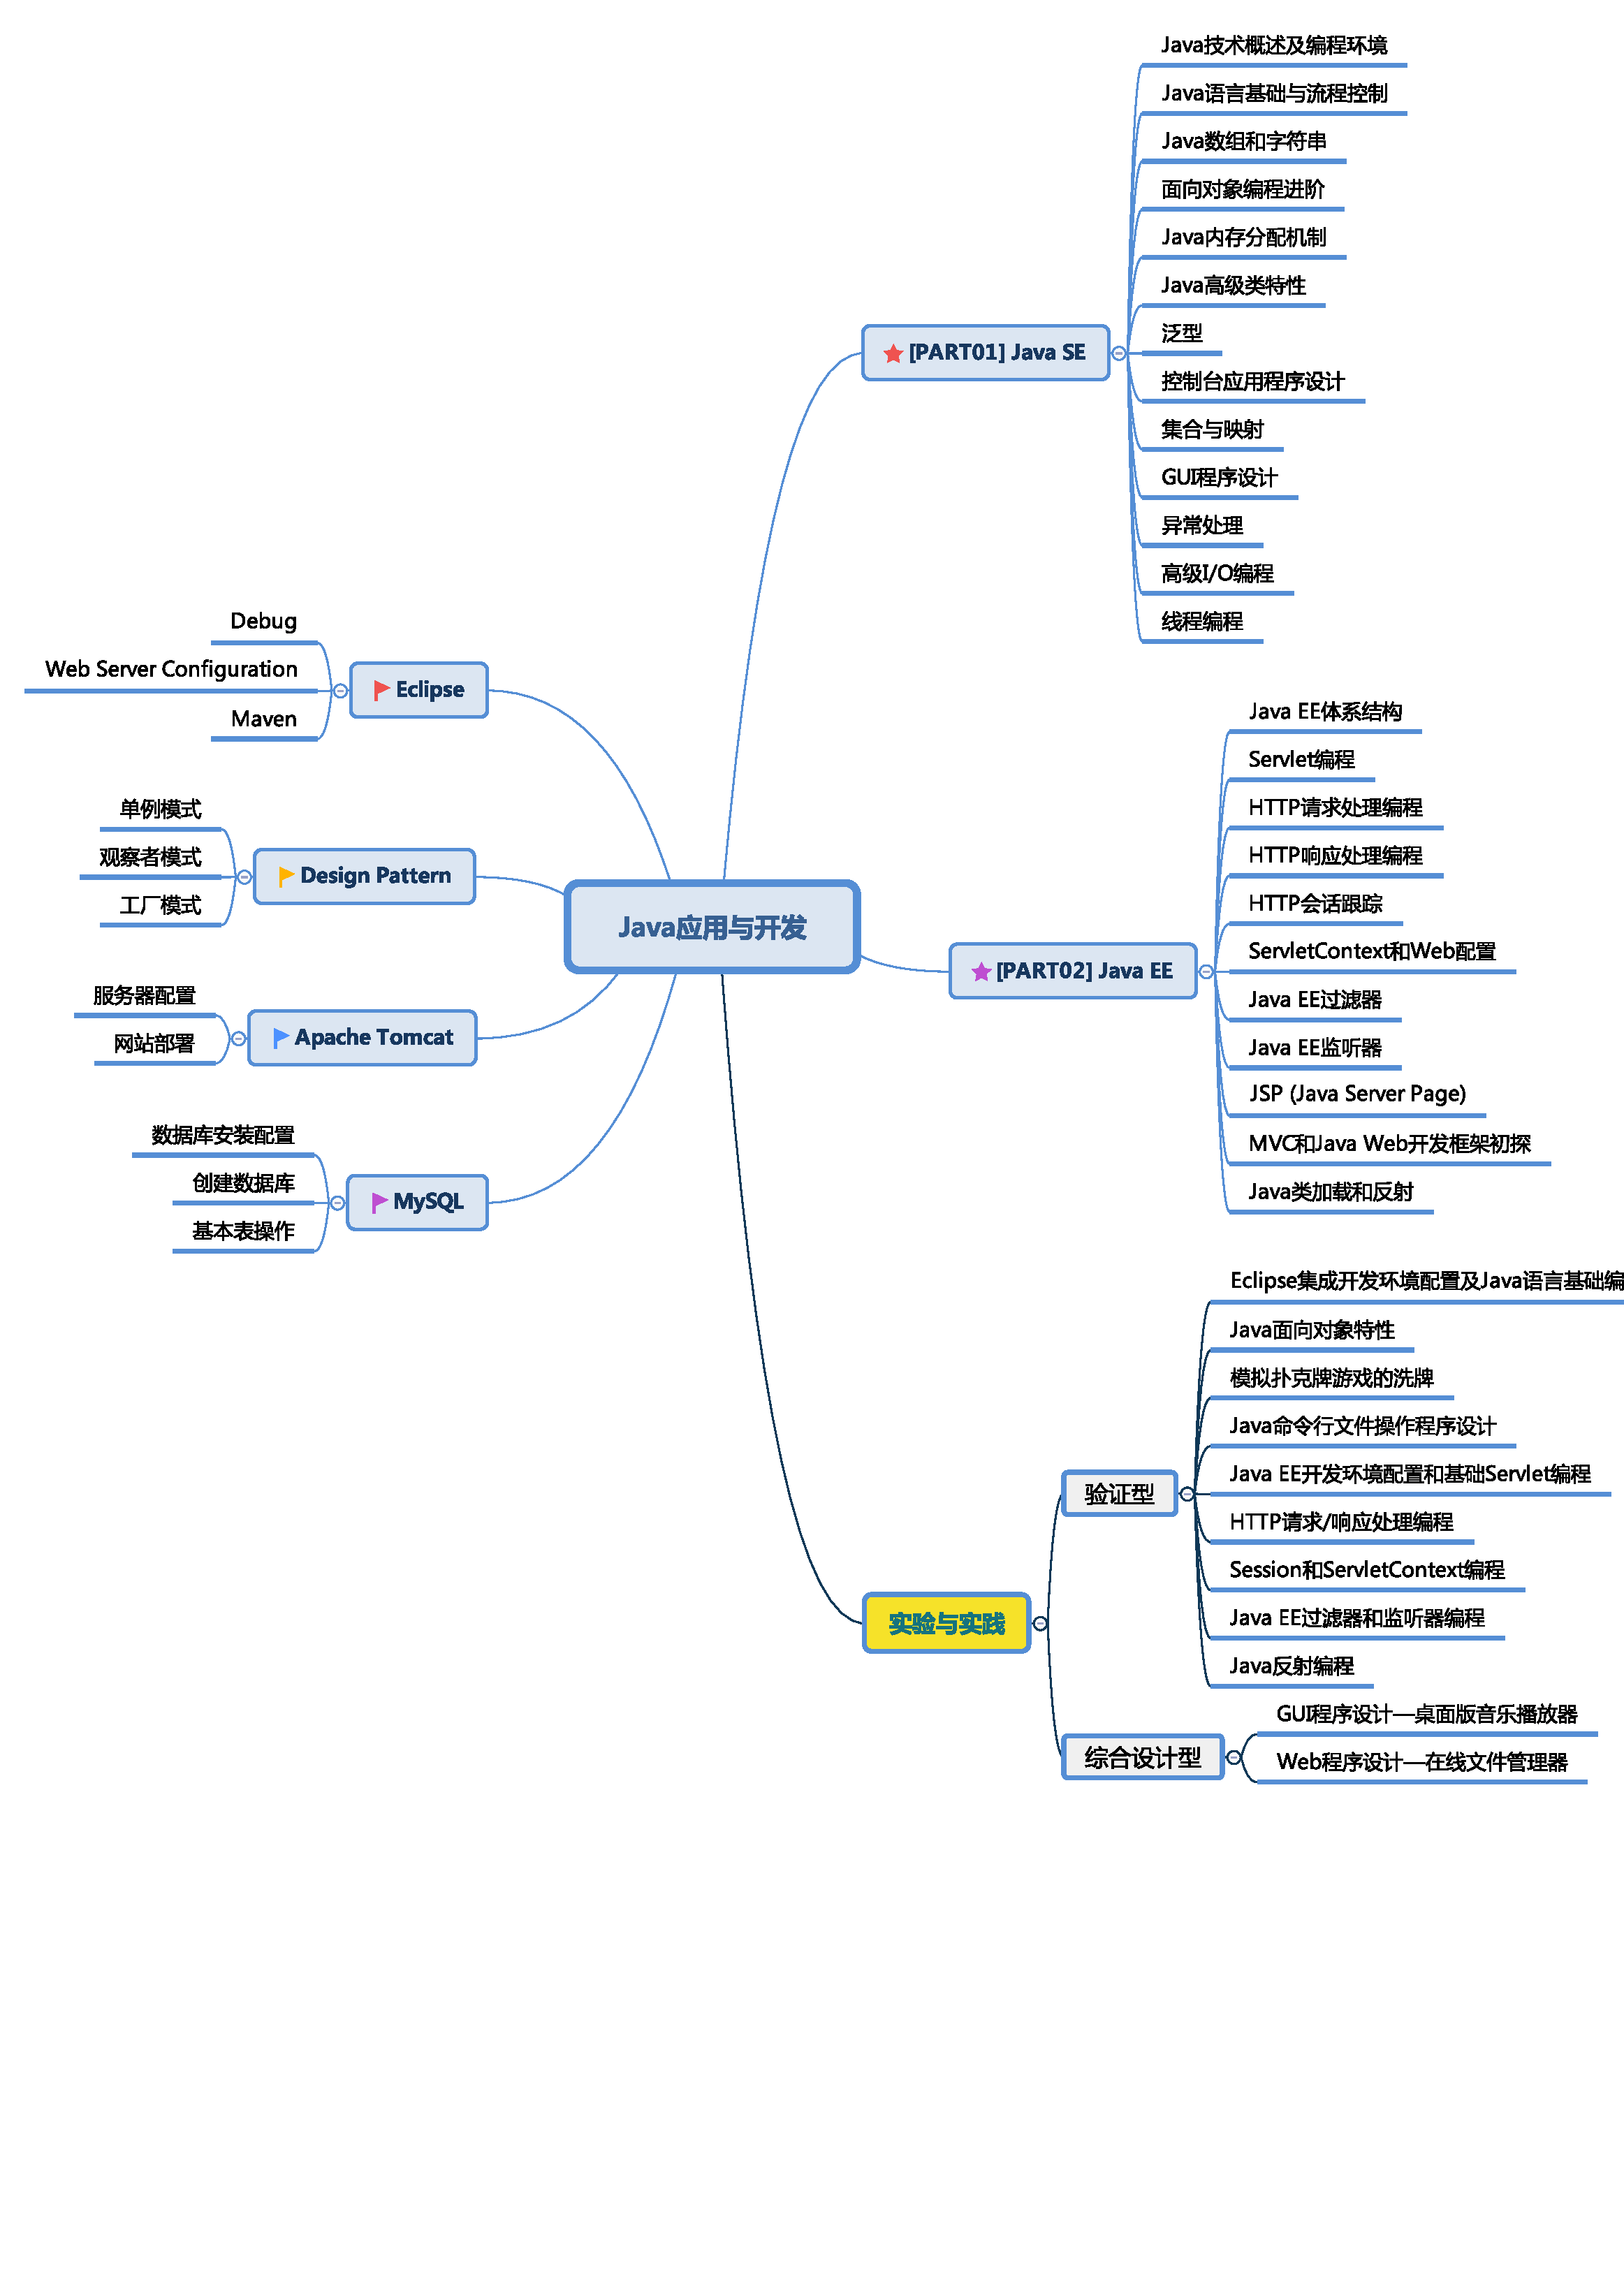
\includegraphics[width=\textwidth]{images/fig-java-course-arch.pdf}
\caption{Java应用与开发课程教学体系}
\label{fig:java-course-arch}
\end{figure}


%% Week 01 %%

\chapter{Java 技术概述及开发环境}
\label{chp:Introduction-to-Java}

\section*{基本信息}
\sline
\begin{description}
\item[课程名称:] Java应用与开发
\item[授课教师:] 王晓东
\item[授课时间:] 第一周
\item[参考教材:] 本课程参考教材及资料如下:
  \begin{itemize}
  \item 陈国君主编,Java程序设计基础(第5版),清华大学出版社,2015.5
  \item Bruce Eckel, Thinking in Java (3rd)
  \end{itemize}
\end{description}

\section*{教学目标}

\sline
\begin{enumerate}
\item 讲解Java的发展历程,从Java的视角回顾OOP;
\item 理解Java平台的相关概念和机制;
\item 掌握基本的Java开发环境配置方法。
\end{enumerate}  

\section*{授课方式}

\sline
\begin{description}
\item[理论课:] 多媒体教学、程序演示
\item[实验课:] 上机编程
\end{description}

\newpage
\section*{教学内容}
\sline

\section{Java技术概述}

\subsection{Java发展简史}

Java的发展过程中伴随着多个伟大公司的起起落落。

\begin{description}
\item[\fbox{1982}] Sun公司成立(安迪$\cdot$贝托谢姆和麦克尼利)。
\item[\fbox{1986}] Sun公司上市。
\item[\fbox{1985}] Sun公司推出著名的Java语言。
\item[\fbox{2001}] 9.11事件前,Sun市值超过1000亿美元;此后,由于互联网泡沫的破碎,其市值
  在一个月内跌幅超过90\%。
\item[\fbox{2004}] Sun公司和微软在旷日持久的Java官司中和解,后者支付前者高达10亿美元的
  补偿费。
\item[\fbox{2006}] 共同创始人麦克尼利辞去CEO一职,舒瓦茨担任CEO后尝试将Sun从设备公司向软
  件服务型公司转型,但不成功。
\item[\fbox{2010}] Sun公司被甲骨文公司收购。
\end{description}

Java语言的版本迭代历程如图\ref{fig:java-versions}所示。

\begin{figure}[htb]
\centering
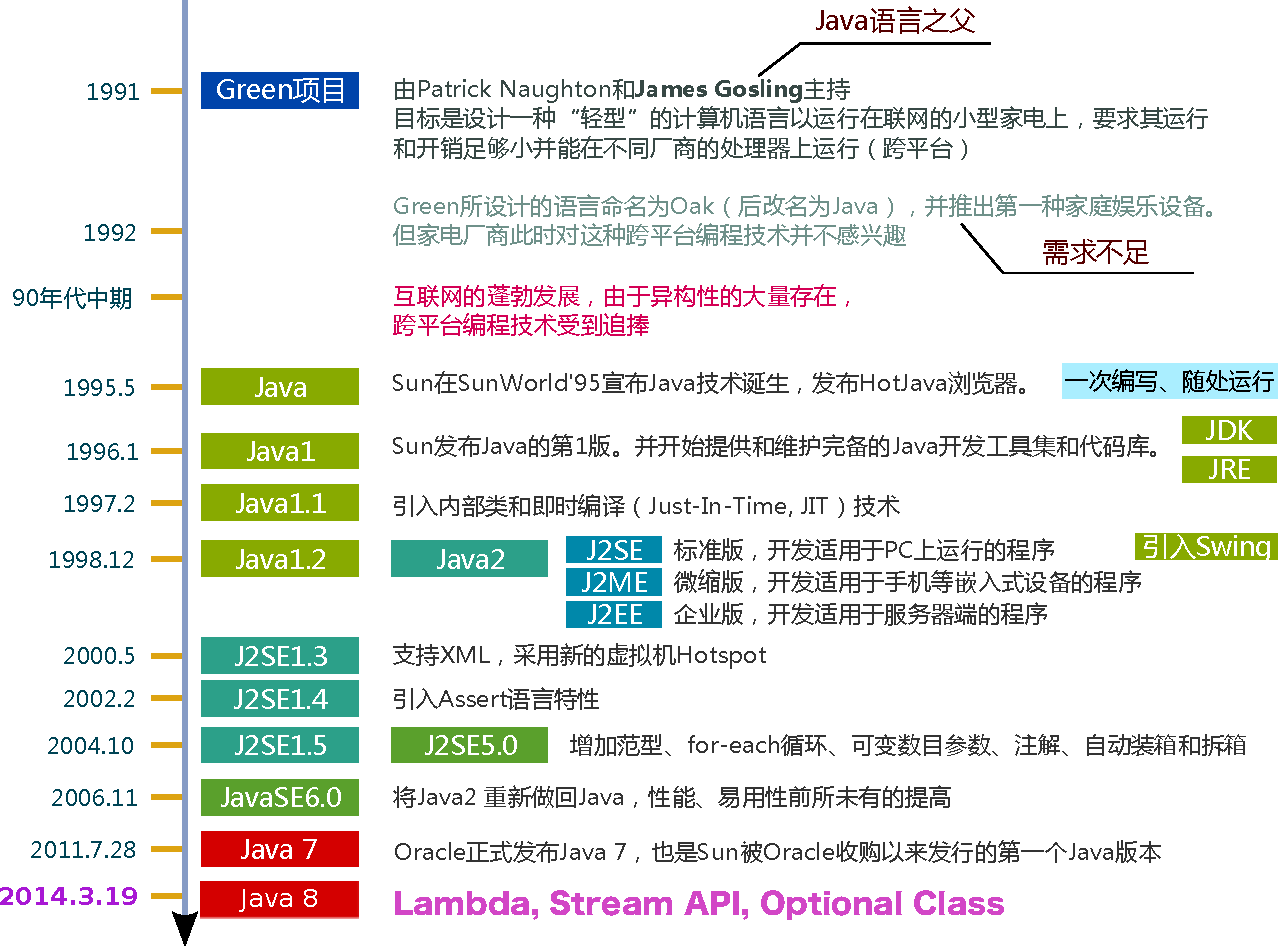
\includegraphics[width=\textwidth]{images/Introduction-to-Java/fig-java-versions.pdf}
\caption{Java版本迭代}
\label{fig:java-versions}
\end{figure}

\subsection{Java技术的特点}

Java具备以下技术特点:

\begin{description}
\item[面向对象] Java是一种以对象为中心,以消息为驱动的面向对象的编程语
  言。
\item[平台无关性] 分为源代码级(需重新编译源代码,如C/C++)和目标代码
  级(Java)平台无关。
\item[分布式] 可支持分布式技术及平台开发。
\item[可靠性] 不支持直接操作指针,避免了对内存的非法访问;自动单元回收
  功能防止内存丢失等动态内存分配导致的问题;解释器运行时实施检查,可发
  现数组和字符串访问的越界;提供了异常处理机制。
\item[多线程] C++没有内置的多线程机制,需调用操作系统的多线程功能来进行
  多线程序设计;Java提供了多线程支持。
\item[网络编程] Java具有丰富的网络编程库。
\item[编译和解释并存] 由编译器将Java源程序编译成字节码文件,再由运行系
  统解释执行字节码文件(解释器将字节码再翻译成二进制码运行)。
\end{description}

\section{Java平台核心机制}


Java技术栈如图\ref{fig:java-tech-stack}所示,程序的编译运行过程如
图\ref{fig:java-running-process}所示。需要了解以下几个核心概念:

\begin{itemize}
\item Java虚拟机
\item 垃圾回收机制
\item Java运行时环境(Java Runtime Environment, JRE)
\item JIT, Just-In-Time 传统解释器的解释执行是转换一条,运行完后就将其扔掉;
  JIT会自动检测指令的运行情况,并将使用频率高(如循环运行)的指令解释后保存下来,下次调用
  时就无需再解释(相当于局部的编译执行),显著提高了Java的运行效率。
\end{itemize}

\begin{figure}[htb]
  \begin{minipage}[t]{0.4\linewidth}
    \centering
    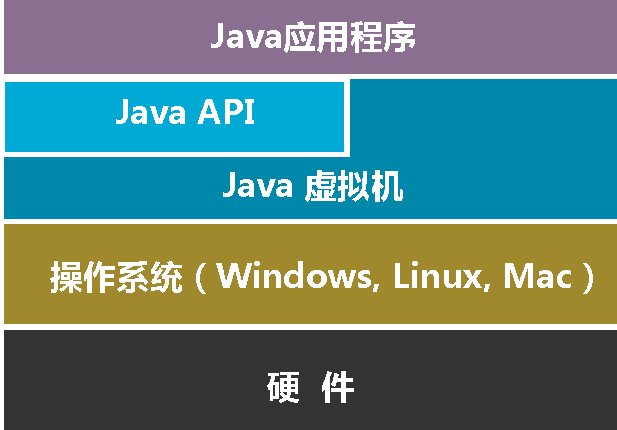
\includegraphics[width=0.9\textwidth]{images/Introduction-to-Java/fig-java-tech-stack.pdf}
    \caption{Java技术栈}
    \label{fig:java-tech-stack}
  \end{minipage}
  \begin{minipage}[t]{0.6\linewidth}
    \centering
    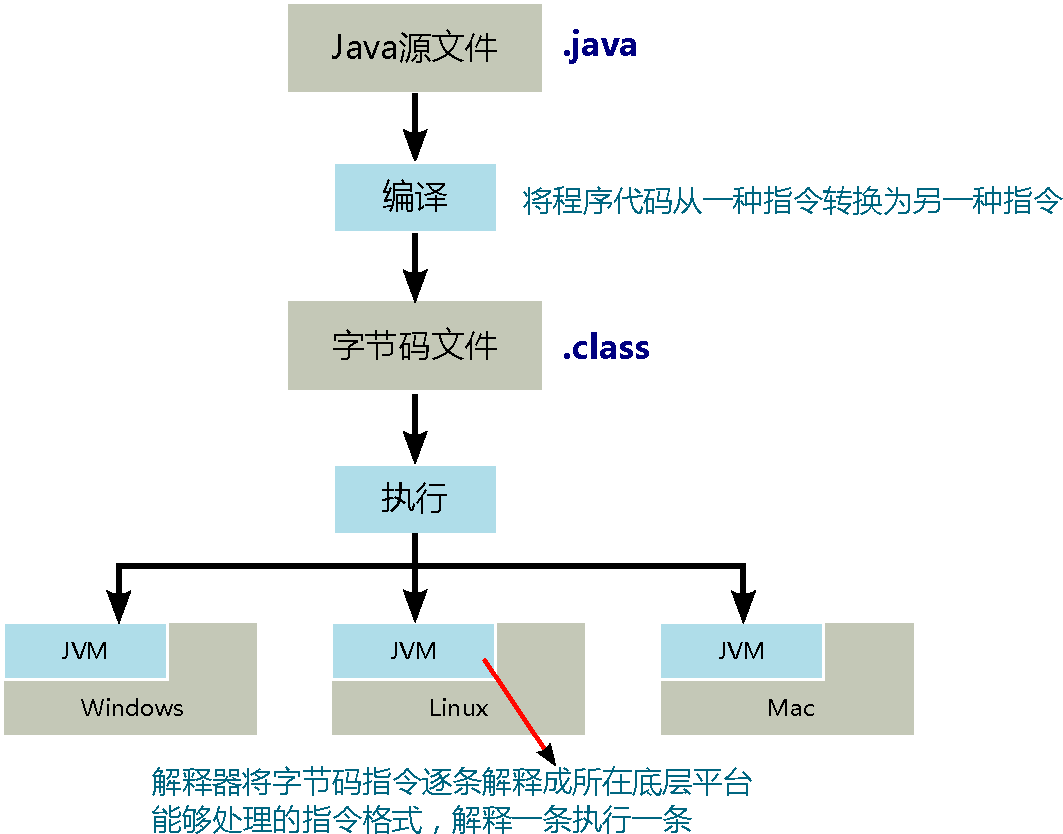
\includegraphics[width=\textwidth]{images/Introduction-to-Java/fig-java-running-process.pdf}
    \caption{Java程序编译运行过程}
    \label{fig:java-running-process}
  \end{minipage}
\end{figure}

\section{Java开发环境}
构建Java开发环境,需要首先获取和安装Java开发工具集,可以从Oracle官方网
站链
接http://www.oracle.com/technetwork/java/javase/downloads/index.html获
取。下载完成后解压放入合适的磁盘目录下。

对于Windows操作系统,可以采用以下路径:

\begin{shCode}
  D:\Program Files\Java
\end{shCode}

对于Linux操作系统,可以采用以下路径:

\begin{shCode}
  /opt/jdk1.8.0_172
\end{shCode}

接下来进行环境变量配置,以Windows操作系统为例:

\begin{description}
\item[\fbox{变量名}] Path
\item[\fbox{变量值}] D:\textbackslash Program Files\textbackslash Java\textbackslash
  jdk1.8.0\_172\textbackslash bin
\end{description}

配置完成后,可以看到JDK目录中包含以下子目录和文件:

\begin{shCode}
  bin  COPYRIGHT  db  include  javafx-src.zip
  jre  lib  LICENSE  man  README.html  release  src.zip
  THIRDPARTYLICENSEREADME-JAVAFX.txt  THIRDPARTYLICENSEREADME.txt  
\end{shCode}

对子目录的功能简要描述如下:

\begin{description}
\item[bin] Java开发工具,包括编译器、虚拟机、调试器、反编译器等;
\item[jre] Java运行时,包括Java虚拟机、类库和其他资源文件;
\item[lib] 类库和所需支持性文件;
\item[include] 用于调试本地方法(底层平台)的C++头文件;
\item[src.zip] 类库的源代码;
\item[db] Java DB数据库,JDK6.0新增项目,一种纯Java的关系型数据库。
\end{description}

\section{Java开发工具}

业界普遍采用Eclipse或IntelliJ IDEA等集成开发环境进行Java大型工程开发,
当然也可以采用文本编程工具Vim或Emacs等进行Java小型程序的开发。

本课程采用Eclipse作为首选集成开发环境。

\section{Java基本开发流程}

本部分使用文本编程工具编写一个简单的Java Hello World程序,演示Java的基
本开发和代码编译运行流程。首先,我们需要使用文本编程工具编写一个Java源
文件HelloWorld.java,文件命名必须与类名相同。

\begin{javaCode}
public class HelloWorld {
    public static void main(String[] args) {
	System.out.println("Hi, Java!");
    }
}   
\end{javaCode}

然后,使用javac工具将源文件编译为字节码文件,编译完成后,我们可以看到生成了HelloWord.class这一字节码文件。

\begin{shCode}
  > javac HelloWorld.java && ls 
  HelloWorld.class  HelloWorld.java
\end{shCode}

接下来,我们使用java工具运行该程序,在终端正确打印了“Hi, Java”字符串。

\begin{shCode}
  > java HelloWorld 
  Hi, Java!
\end{shCode}


\descript{说明}

编写Java应用程序需掌握的几条规则如下:

\begin{enumerate}
\item Java语言拼写是大小写敏感的(Case-Sensitive);
\item 一个源文件中可以定义多个Java类,但其中最多只能有一个类被定义为Public类;
\item 如果源文件中包含了public类,则源文件必须和该public类同名;
\item 一个源文件包含多个Java类时,编译后会生成多个字节码文件,即每个类都会生成一个单独的
  “.class”文件,且文件名与类名相同。
\end{enumerate}


\chapter{Java 语言基础与流程控制}
\label{chp:Java-language-basic-and-flow-control}

\section*{基本信息}
\sline
\begin{description}
\item[课程名称:] Java应用与开发
\item[授课教师:] 王晓东
\item[授课时间:] 第一周
\item[参考教材:] 本课程参考教材及资料如下:
  \begin{itemize}
  \item 陈国君主编,Java程序设计基础(第5版),清华大学出版社,2015.5
  \item Bruce Eckel, Thinking in Java (3rd)
  \end{itemize}
\end{description}

\section*{教学目标}

\sline

\begin{enumerate}
\item Java语言基础包括:数据类型、常量和变量、关键字与标识符、运算符与表达式、从键盘输入数据。
\item Java流程控制包括:语句和复合语句、分支结构(选择结构)、循环结构、跳转语句。
\end{enumerate}

\section*{授课方式}

\sline
\begin{description}
\item[理论课:] 多媒体教学、程序演示
\item[实验课:] 上机编程
\end{description}

\newpage
\section*{教学内容}
\sline

\section{Java语言基础}

\subsection{数据类型}

Java数据类型分为两大类:基本数据类型和引用数据类型。基本数据类型是由程
序设计语言系统所定义、不可再划分的数据类型。所占内存大小固定,与软硬件
环境无关,在内存中存放的是数据值本身。Java的基本数据类型包括:整型
(byte、short、int、long)、浮点型(float、double)、逻辑型(boolean)和字
符型(char)。引用数据类型(复合数据类型)在内存中存放的是指向该数据的
地址,不是数据值本身。引用数据类型包括类、数组、接口等。

数据类型的基本要素包括:

\begin{itemize}
\item 数据的性质(数据结构)
\item 数据的取值范围(字节大小)
\item 数据的存储方式
\item 参与的运算
\end{itemize}



\subsubsection{整型}

Java整型类型的数据位数及取值范围如表\ref{tab:integer-type}所示。

\begin{table}[!htbp]
  \centering
  \caption{整型数据类型}
  \label{tab:integer-type}
  \begin{tabular}{|c|c|l|}
    \hline
    {\bf 类型} & {\bf 数据位数} & {\bf 取值范围}   \\
    \hline
    byte(字节型) & 8 & $-128 \sim 127$,即$-2^{7} \sim 2^{7}-1$\\
    \hline
    short(短整型) & 16 & $-32768 \sim 32767$,即$-2^{15} \sim 2^{15}-1$\\
    \hline
    int(整型)(默认) & 32 & $-2147483648 \sim 2147483647$,即$-2^{31} \sim 2^{31}-1$\\
    \hline
    long(长整型)(l或L) & 64 & $-2^{63} \sim 2^{63}-1$\\
    \hline
  \end{tabular}
\end{table}

\subsubsection{浮点型}

Java浮点型类型的数据位数及取值范围如表\ref{tab:float-type}所示。

\begin{table}[!htbp]
  \centering
  \caption{整型数据类型}
  \label{tab:float-type}
  \begin{tabular}{|c|c|l|}
    \hline
    {\bf 类型} & {\bf 数据位数} & {\bf 取值范围}   \\
    \hline
    float(单精度)(f或F) & 32 & $1.4E-45 \sim 3.4E+38$\\
    \hline
      double(双精度)(默认) & 64 & $4.9E-324 \sim 1.8E+308$\\
    \hline
  \end{tabular}
\end{table}

\subsubsection{逻辑型}

逻辑型又称为布尔型(boolean),布尔型数据类型的特性如下:

\begin{itemize}
\item 布尔型数据只有true(真)和false(假)两个取值。
\item 布尔型数据存储占1个字节,默认取值为false。
\item 布尔型数据true和false不能转换成数字表示形式。
\end{itemize}

\subsubsection{字符型}

\begin{itemize}
\item 字符型数据类型用来存储单个字符,采用的是Unicode字符集编码方
  案\footnote{建议搜索理解什么是字符集和字符编码规则。}。
\item 字符声明用单引号表示单个字符。
\item 字符型数据可以转化为整型。
\end{itemize}

\samplecode{字符数据类型示例}
  
\begin{javaCode}
  public class CharDemo {
    public static void main(String[] args) {
      char a = 'J';
      char b='Java';  //会报错
    }
  }
\end{javaCode}
 
\subsection{数据类型转换}

\subsubsection{数值型不同类型数据的转换}

数值型不同类型数据之间的转换,{\hei 自动类型转换}需要符合以下条件:

\begin{enumerate}
\item 转换前的数据类型与转换后的类型兼容。
\item 转换后的数据类型的表示范围比转换前的类型大。
\item 条件2说明不同类型的数据进行运算时,需先转换为同一类型,然后进行运算。转换从“短”到“长”的优先关系为:\\
  byte → short → char → int → long → float → double
\end{enumerate}

如果要将较长的数据转换成较短的数据时(不安全)就要进行{\hei 强制类型转换},格式如下:

\begin{javaCode}
  (预转换的数据类型) 变量名;
\end{javaCode}

\subsubsection{字符串型数据与数值型数据相互转换}

\samplecode{字符串数据转换为数值型数据示例}

\begin{javaCode}
  String myNumber = "1234.56";
  float myFloat = Float.parseFloat(MyNumber);
\end{javaCode}

字符串可用加号“+”来实现连接操作。若其中某个操作数不是字符串,该操作在
连接之前会自动将其转换成字符串。所以可用加号来实现自动的转换。

\samplecode{数值型数据转换成字符串数据示例}

\begin{javaCode}
  int myInt = 1234;               //定义整形变量MyInt
  String myString = "" + MyInt;    //将整型数据转换成了字符串 
\end{javaCode}

\subsection{常量和变量}



\subsubsection{常量}

\begin{description}
\item[整型常量] 八进制、十六进制、十进制长整型后需要加l或L。
\item[浮点型常量] 单精度后加f或F,双精度后加d或D可省略。
\item[逻辑型常量] true或者false。
\item[字符型常量] 单引号。
\item[字符串常量] 双引号。
\end{description}

\samplecode{常量的声明}

\begin{javaCode}
  final int MAX = 10;
  final float PI =3.14f;
\end{javaCode}

\subsubsection{变量}

变量的属性包括变量名、类型、值和地址。Java语言程序中可以随时定义变量,不必集中在执行语句之前。

\samplecode{变量声明、初始化和赋值}

\begin{javaCode}
  int i, j = 0;
  i = 8;
  float k;
  k = 3.6f;
\end{javaCode}


\subsection{关键字与标识符}

Java的关键字(Java保留字)如表\ref{tab:java-key-word}所示。

\begin{table}[!htbp]
  \centering
  \caption{Java语言的关键字(保留字)}
  \label{tab:java-key-word}
  \begin{tabular}{|c|c|c|c|c|c|}
    \hline
    abstract & assert & boolean & break & byte & case \\
    \hline
    catch & char & class & continue & default & do \\
    \hline
    double & else & enum & extends & false & final \\
    \hline    
    finally & float & for & if & implements & import \\
    \hline
    instanceof & int & interface & long & native & new \\
    \hline
    null & package & private & protected & public & return \\
    \hline
    short & static & super & switch & synchronized & this \\
    \hline
    volatile & throws & transient & true & try & void \\
    \hline
  \end{tabular}
\end{table}

标识符是用来表示变量名、类名、方法名、数组名和文件名的有效字符序列。Java语言对标识符的规定如下:
  
\begin{itemize}
\item 可以由字母、数字、下划线(\_)、美元符号(\$)组合而成。
\item 必须以字母、下划线或美元符号开头,不能以数字开头。
\item 关键字不能当标识符使用。
\item 区分大小写。
\end{itemize}

建议遵循驼峰命名,类名首字母大写,变量、方法及对象首字母小写的编码习惯。

\subsection{运算符与表达式}

按照运算符功能来分,Java基本的运算符包括以下几类:

\begin{figure}[htb]
\centering
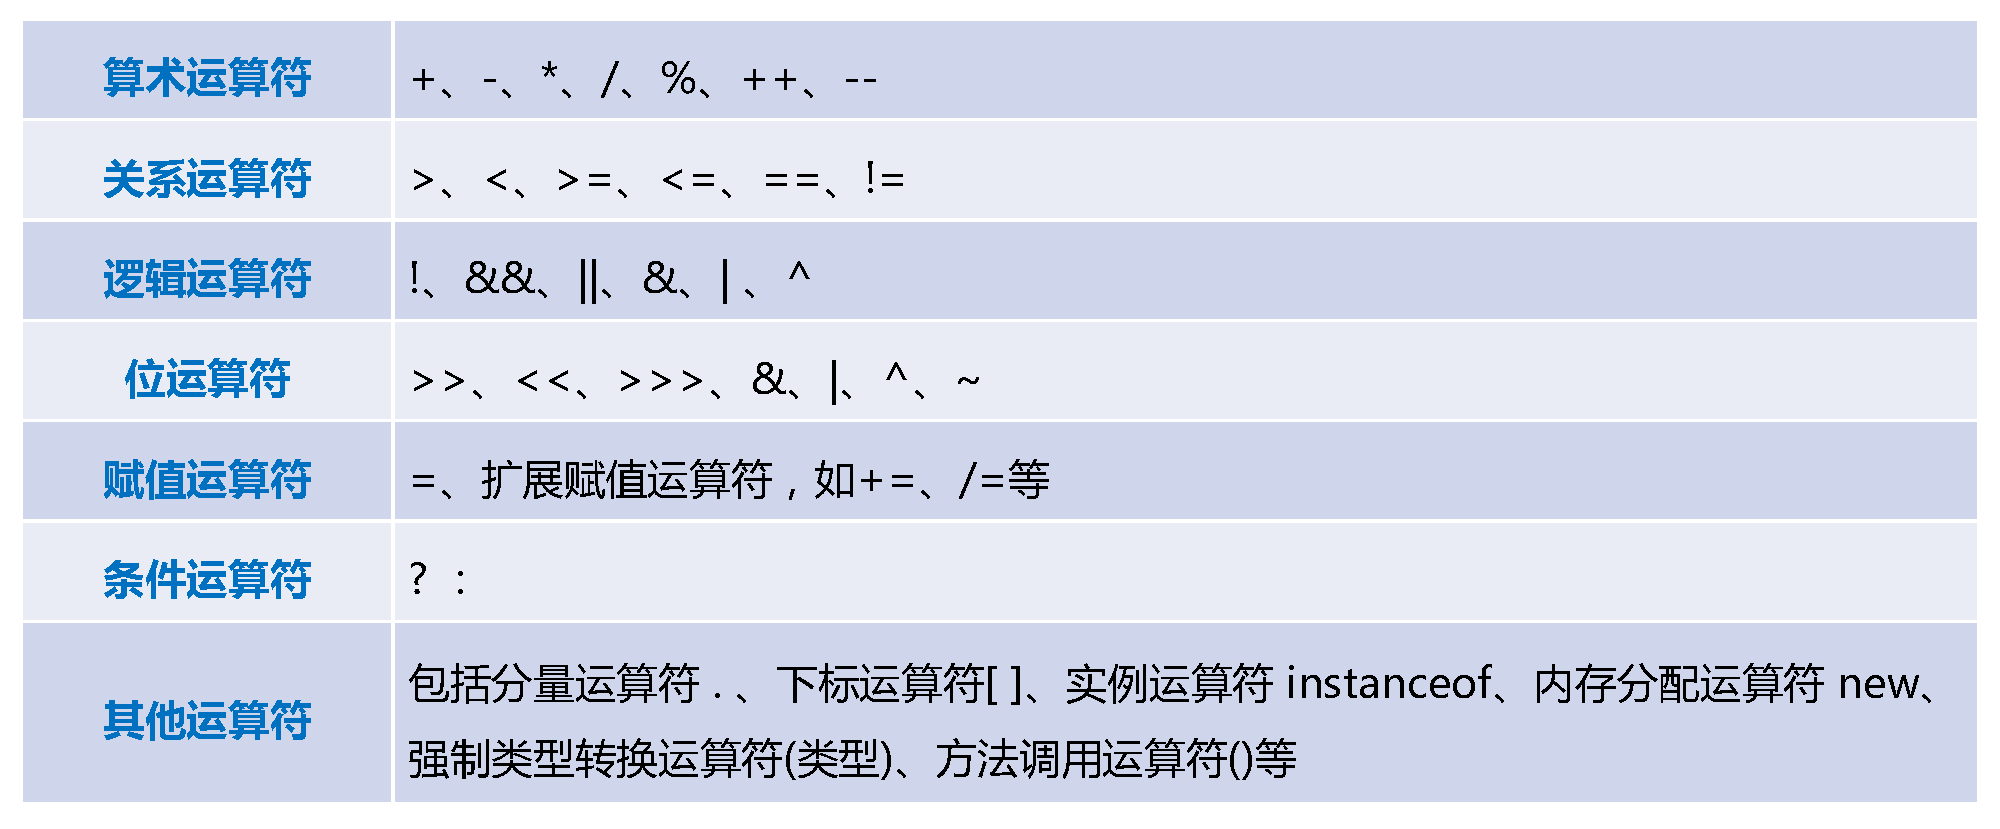
\includegraphics[width=0.9\textwidth]{images/Java-language-basic-and-flow-control/fig-java-operators.pdf}
\caption{Java运算符}
\label{fig:java-operators}
\end{figure}
  
\subsection{从键盘获得输入}

由键盘输入的数据,不管是文字还是数字,Java皆视为{\hei\Red 字符串},若是要由键盘输入获得数字则必须再经过类型转换。

\samplecode{获得键盘输入字符串并转换为数字}

\begin{javaCode}
  import java.io.*;
  public class MyClass {
    public static void main(String[] args) throws IOException {
      int num1, num2;
      String str1, str2;
      InputStreamReader in;
      in = new InputStreamReader(System.in);
      BufferedReader buf;
      buf = new BufferedReader(in);
      System.out.print("请输入第一个数:");
      str1 = buf.readLine();         //将输入的内容赋值给字符串变量 str1
      num1 = Integer.parseInt(str1);   //将 str1 转成 int 类型后赋给 num1
      System.out.print("请输入第二个数:");
      str2 = buf.readLine();         //将输入的内容赋值给字符串变量 str2
      num2 = Integer.parseInt(str2);   //将 str2 转成 int 类型后赋给 num2
      System.out.println(num1 + " * " + num2 + " = " + (num1 * num2));
    }
  }
\end{javaCode}

为了简化输入操作,从JavaSE 5版本开始在java.util类库中新增了一个类专门用
于输入操作的类{\bf\Red Scanner},可以使用该类输入一个对象。

\samplecode{使用Scanner获得键盘输入并转换为特定数据类型}

\begin{javaCode}
  import java.util.*;
  public class MyClass {
    public static void main(String[] args)
    {
      Scanner reader = new Scanner(System.in); 
      double num;
      num = reader.nextDouble(); //按照 double 类型读取键盘输入
      ...
    }
  }
\end{javaCode}

Scanner对象其他可用的数据读取方法包
括:nextByte()、nextDouble()、nextFloat()、nextInt()、nextLong()、
nextShort()、next()、nextLine()。

\section{Java流程控制}

\subsection{语句与复合语句}

\begin{itemize}
 \item Java语言中语句可以是以分号“;”结尾的简单语句,也可以是用一对花括号“\{\}”括起来的复合语句。
 \item Java中的注释形式:
   \begin{itemize}\small\Blue
   \item 单行注释://
   \item 多行注释:/*    */
   \item 文件注释:/**   */
   \end{itemize}
\end{itemize}

\subsection{分支结构}

\subsubsection{if分支结构 1}

\begin{figure}[htb]
\centering
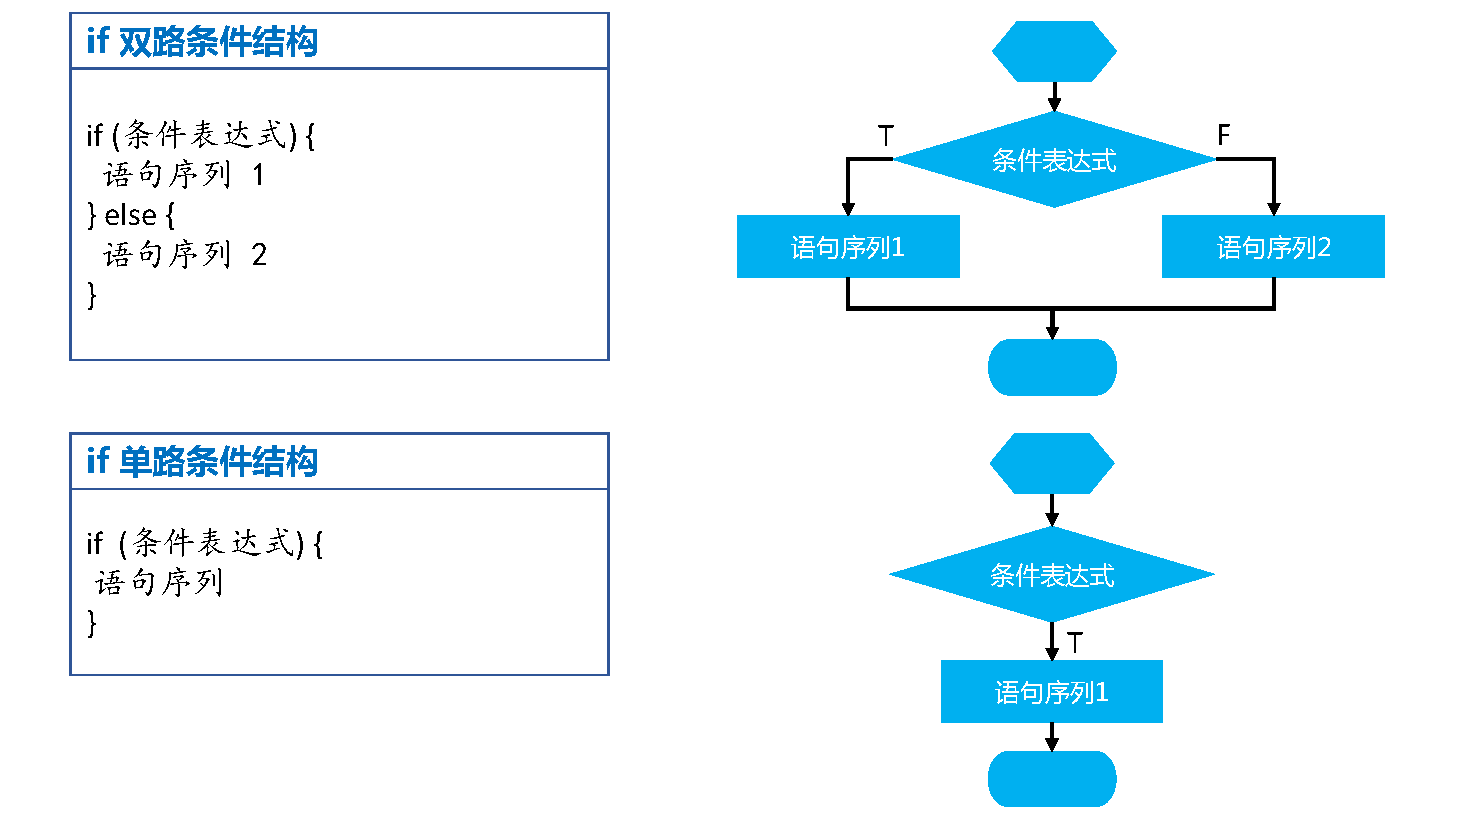
\includegraphics[width=0.9\textwidth]{images/Java-language-basic-and-flow-control/fig-if-branch-1.pdf}
\caption{if分支结构 1}
\label{fig:if-branch-1}
\end{figure}

\subsubsection{if分支结构 2}

\begin{figure}[htb]
\centering
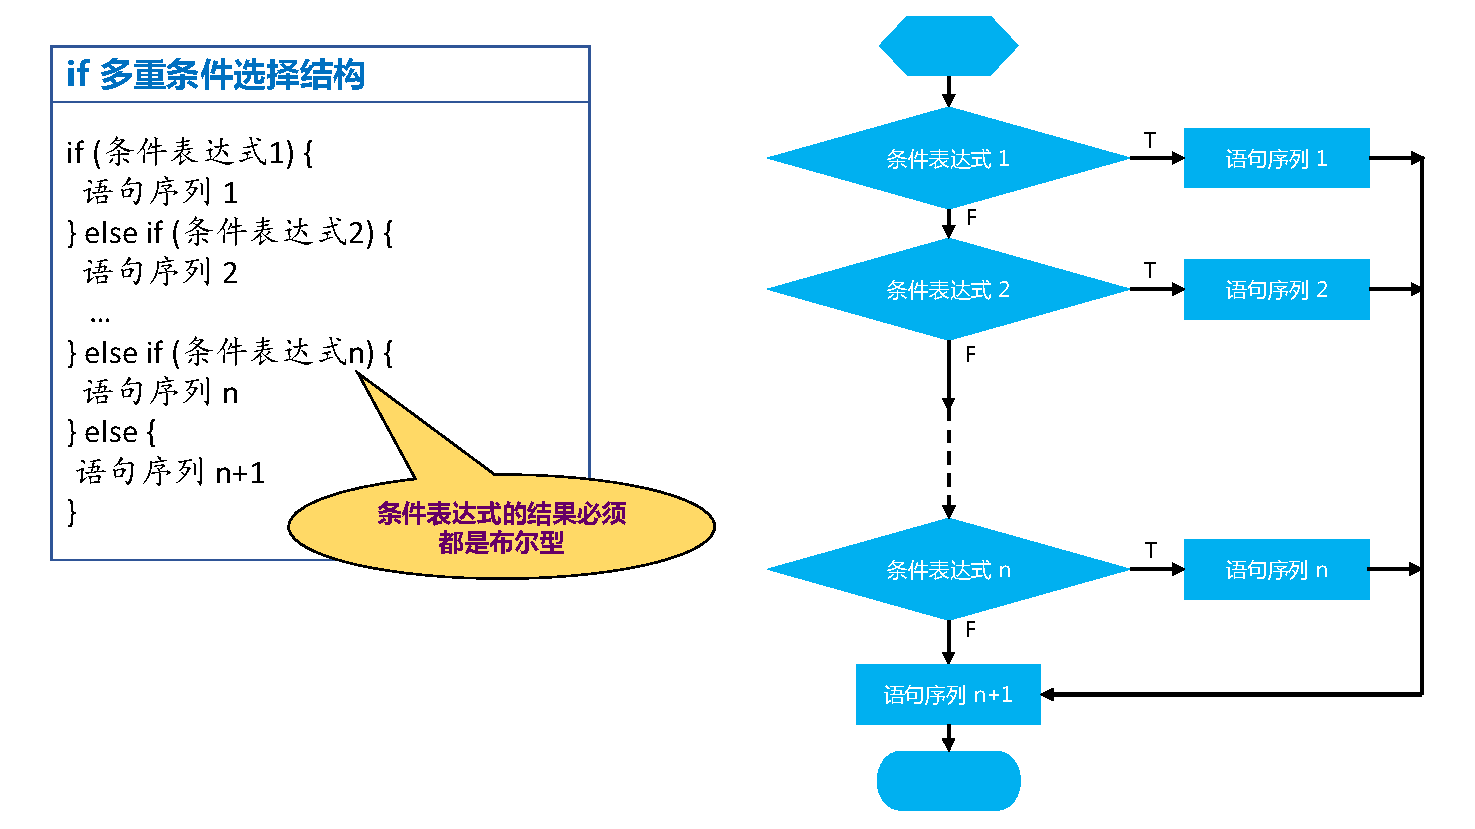
\includegraphics[width=0.9\textwidth]{images/Java-language-basic-and-flow-control/fig-if-branch-2.pdf}
\caption{if分支结构 2}
\label{fig:if-branch-2}
\end{figure}

\subsubsection{switch分支结构}

\begin{figure}[htb]
\centering
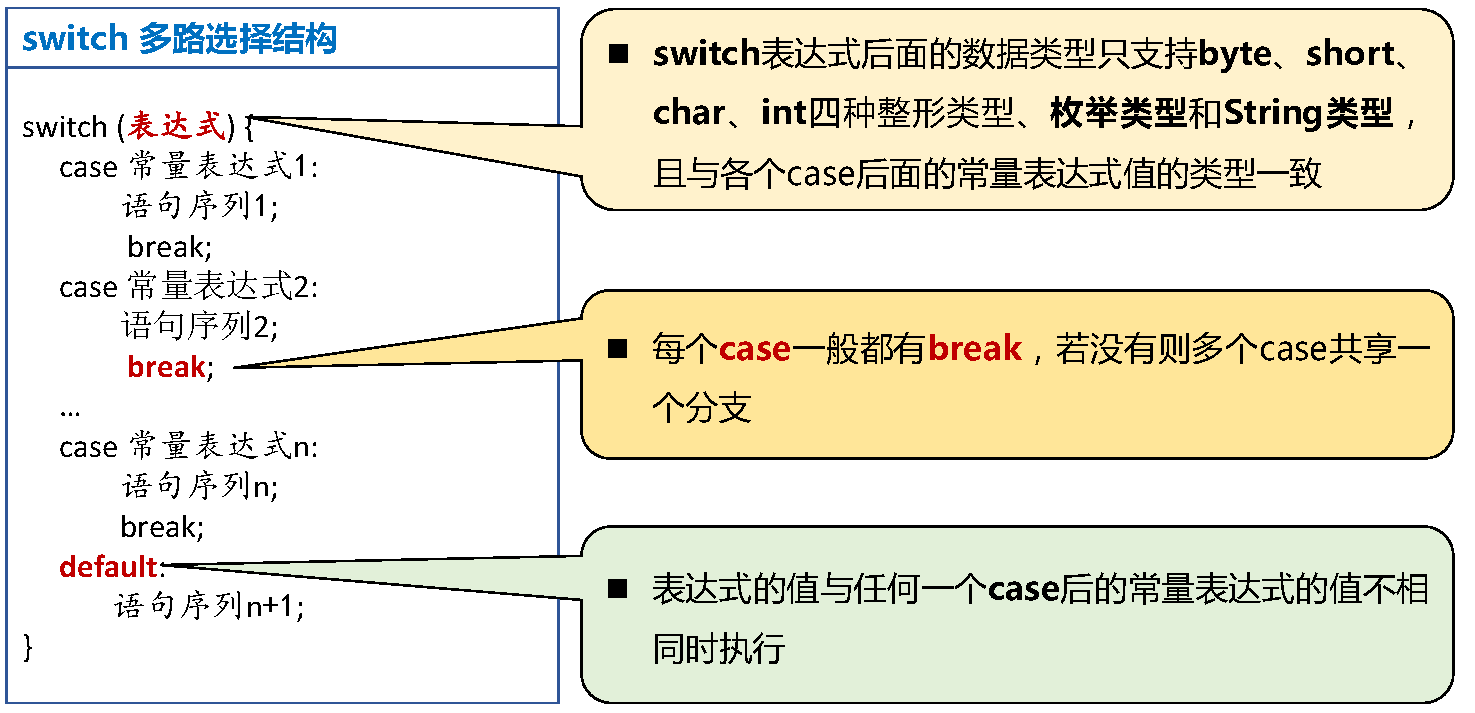
\includegraphics[width=0.9\textwidth]{images/Java-language-basic-and-flow-control/fig-switch-branch.pdf}
\caption{switch分支结构}
\label{fig:switch-branch}
\end{figure}

\descript{说明}

在Java 1.7版本之后,switch里表达式的类型可以为String。

\subsection{循环结构}

\subsubsection{while循环}

\begin{javaCode}
  while(conditional expression) {
    statements goes here ...
  }
\end{javaCode}

\subsubsection{do-while循环}

\begin{javaCode}
  do {
    statements goes here ...
  }
  while(conditional expression);
\end{javaCode}

\subsubsection{for循环 1}

\begin{javaCode}
  int[] integers = {1, 2, 3, 4};
  
  for (int j = 0; j < integers.length; j++) {
    int i = integers[j];
    System.out.println(i);
  } 
\end{javaCode}

\subsubsection{for循环 2}

\begin{javaCode}
  int[] integers = {1, 2, 3, 4};

  for (int i : integers) {
    System.out.println(i);
  }
\end{javaCode}


\subsubsection{循环中的跳转}

\begin{description}
\item[break语句] 使程序的流程从一个语句块(switch或循环结构)内跳出。
\item[continue语句] 终止当前这一轮(次)的循环,进入下一轮(次)循环。
\item[return语句] 用来使程序从方法(函数)中返回,可返回一个值。
\end{description}


\section{课后习题}

\subsection{简答题}
\begin{enumerate}
\item Java语言定义类哪些基本数据类型?其存储结构分别是什么样的?
\item 自动类型转换的前提是什么?转换时的优先级顺序如何?
\item 数字字符串转换为数值类型数据时,可以使用的方法有哪些?
\end{enumerate}

\subsection{小编程}
\begin{enumerate}
\item 编写程序,从键盘输入一个浮点数,然后将该浮点数的整数部分输出。
\item 编写程序,从键盘输入2个整数,然后计算它们相除后得到的结果并输出,注意排除0除问题。
\end{enumerate}
\chapter*{实验设计}
\sline

\begin{description}
\item[实验名称:] Eclipse集成开发环境配置及Java语言基础编程练习
\item[上机时间:] 第一周
\item[实验手册:] 无(参照实验内容完成)
\item[实验内容:] 本次实验需要完成以下内容:
  \begin{enumerate}
  \item 使用文本编辑器完成Java Hello World程序编写,使用javac和java编译运行该程序;
  \item 熟悉Eclipse集成开发环境,学习创建Java工程,使用Maven创建Java工程;
  \item 根据授课幻灯片和讲义,尝试实现其中所有的示例代码。
  \end{enumerate}
  
\item[实验要求:] 本次实验不需要提交实验报告。
\end{description}

%% Week 02 %%
\chapter{Java 数组和字符串}
\label{chp:Java-array-and-string}

\section*{基本信息}
\sline
\begin{description}
\item[课程名称:] Java应用与开发
\item[授课教师:] 王晓东
\item[授课时间:] 第二周
\item[参考教材:] 本课程参考教材及资料如下:
  \begin{itemize}
  \item 陈国君主编,Java程序设计基础(第5版),清华大学出版社,2015.5
  \item Bruce Eckel, Thinking in Java (3rd)
  \end{itemize}
\end{description}

\section*{教学目标}

\sline

\begin{enumerate}
\item 掌握Java数组的概念
\item 学会一维数组和二维数组的使用;认识Arrays类,掌握操作数组相关方法
\item 掌握Java字符串的概念,字符串与数组的关系;学会String类常用字符串操作方法
\end{enumerate}

\section*{授课方式}

\sline
\begin{description}
\item[理论课:] 多媒体教学、程序演示
\item[实验课:] 上机编程
\end{description}

\newpage
\section*{教学内容}
\sline

\section{数组的概念}

数组是相同数据类型的元素按一定顺序排列的集合。在Java语言中,数组元素既可以为基本数据类型,也可以为对象。

\kgtip{Java的内存分配(基础)}

\begin{description}
\item [栈内存] 存放定义的基本类型的变量和对象的引用变量,超出作用域将自动释放。
\item [堆内存] 存放由new运算符创建的对象和数组,由Java虚拟机的自动垃圾回收器来管理。
\end{description}

Java数组的主要特点包括以下方面:

\begin{itemize}
\item 数组是相同数据类型的元素的集合;
\item 数组中的各元素有先后顺序,它们在内存中按照这个先后顺序连续存放;
\item 数组的元素用整个数组的名字和它自己在数组中的顺序位置来表示。
\end{itemize}

{\Blue\kai 例如,a[0]表示名字为a的数组中的第一个元素,a[1]表示数组a的第二个元素,依次类推。}

\section{一维数组}

\subsection{创建数组}

创建Java数组一般需经过三个步骤:

\begin{enumerate}
\item 声明数组;
\item 创建内存空间;
\item 创建数组元素并赋值。
\end{enumerate}

\samplecode{一维数组创建声明和内存分配}

\begin{javaCode}
  int[] x;  //声明名称为x的int型数组,未分配内存给数组
  x = new int[10];   //x中包含有10个元素,并分配空间
\end{javaCode}

\begin{javaCode}
  int[] x = new int[10];   //声明数组并动态分配内存
\end{javaCode}

\descript{说明}

用new分配内存的同时,数组的每个元素都会自动赋默认值,整型为0,实数为0.0,布尔型为false,引用型为null。

\subsection{一维数组的初始化}

若在声明数组时进行赋值即初始化,称为静态内存分配。

\begin{javaCode}
  数据类型[] 数组名 = {初值0,初值1,…,初值n};
\end{javaCode}

\samplecode{一维数组静态初始化}

\begin{javaCode}
  int[] a = {1,2,3,4,5};
\end{javaCode}

\descript{注意}

在Java程序中声明数组时,无论用何种方式定义数组,都不能指定其长度。

\section{二维数组}

Java中无真正的多维数组,只是数组的数组。

\subsection{二维数组的声明和内存分配}

\begin{javaCode}
  数据类型[][] 数组名;
  数组名 = new 数据类型 [行数][列数];
  数据类型[][] 数组名 = new 数据类型 [行数][列数];
\end{javaCode}

\begin{figure}[htb]
\centering
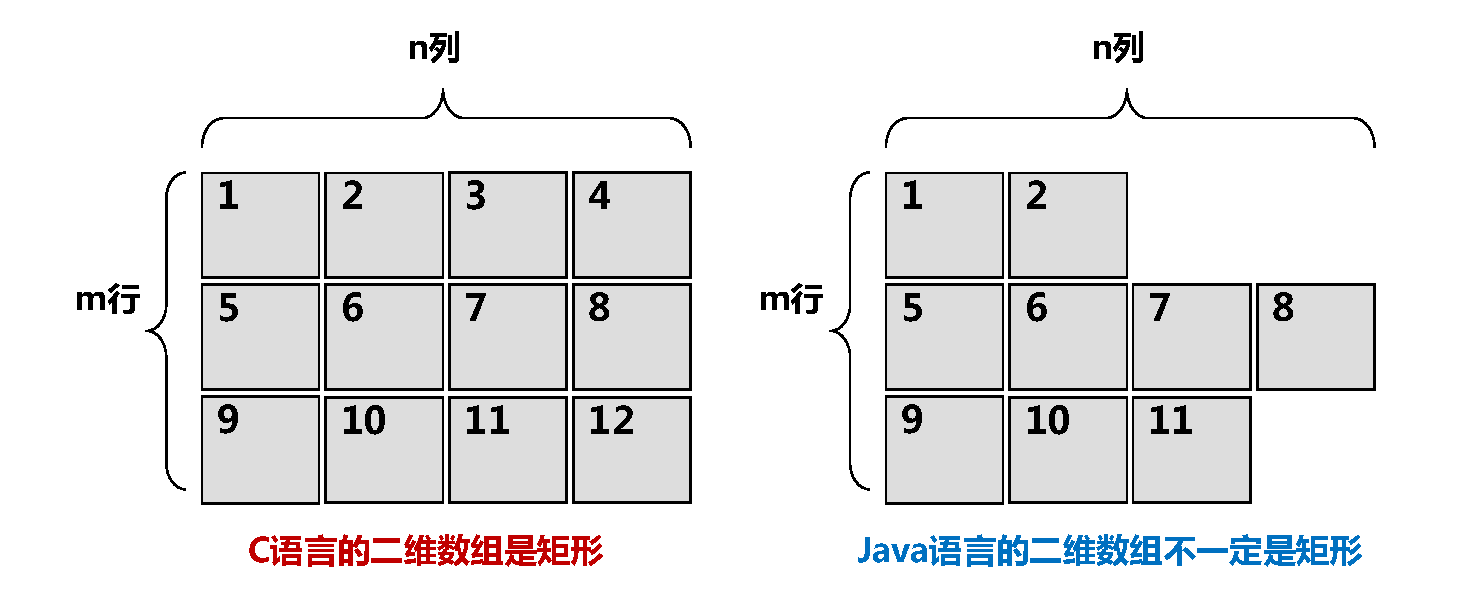
\includegraphics[width=\textwidth]{images/Java-array-and-string/fig-2-dim-array.pdf}
\caption{Java版本迭代}
\label{fig:java-versions}
\end{figure}

\subsection{二维数组定义的含义}

\begin{itemize}
\item Java中的二维数组看作是由多个一维数组构成
\item 二维数组申请内存必须指定{\Red 高层维数}\\
  \fbox{int[][] myArray1 = new int[10][];}\\
  \fbox{int[][] myArray2 = new int[10][3];}
\item \fbox{int[][] x;}\\
  {\kai\Blue 表示定义了一个数组引用变量x,第一个元素为x[0],最后一个为x[n-1],其长度不确定}
\item \fbox{x = new int[3][];}\\
  {\kai\Blue 表示数组x有三个元素,每个元素都是int[]类型的一维数组,分别为int x[0][]、int[] x[1]、int[] x[2]}\\
  \fbox{x[0] = new int[3];  x[1] = new int[2];}\\
  {\kai\Blue 给x[0]、x[1]、x[2]赋值(长度可以不一样)}
\end{itemize}

\subsection{二维数组赋初值}

\begin{javaCode}
  int[][] a = {{11,22,33,44}, {66,77,88,99}};
\end{javaCode}

\descript{注意}

声明多维数组并初始化时不能指定其长度,否则出错。



\section{Arrays类}

java.util.Arrays工具类能方便地操作数组,它提供的所有方法都是静态的。该类具有以下功能:

\begin{description}
\item[给数组赋值] 通过fill方法。
\item[对数组排序] 通过sort方法。
\item[比较数组] 通过equals方法比较数组中元素值是否相等。
\item[查找数组元素] 通过binarySearch方法能对排序好的数组进行二分查找法操作。
\item[复制数组] 把数组复制成一个长度为length的新数组。
\end{description}

\samplecode{Array操作示例}

\begin{javaCode}
  /*
  * 数组比较 equals
  */
  String[] str1 = { "1", "2", "3" };
  String[] str2 = { "1", "2", new String("3") };
  System.out.println(Arrays.equals(str1, str2)); // 结果是true

  /*
  * 数组排序 sort
  */
  int[] score = { 79, 65, 93, 64, 88 };

  // 将数组转换为字符串
  String str = Arrays.toString(score);
  System.out.println("原数组为:" + str);

  Arrays.sort(score); // 作用是把一个数组按照有小到大进行排序,会改变原score而不是创建新对象

  // 将数组转换为字符串
  System.out.println("排序后数组为:" + Arrays.toString(score));

  /*
  * 把数组中的所有元素替换成一个值 fill
  */
  int[] num = { 1, 2, 3 };
  Arrays.fill(num, 6); // 参数1:数组对象;参数2:替换的值
  System.out.println(Arrays.toString(num)); // 打印结果:[6, 6, 6]

  /*
  * 通过二分法查询元素值在数组中的下标 binarySearch
  */
  char[] a = { 'a', 'b', 'c', 'd', 'e' };
  int i = Arrays.binarySearch(a, 'd');
  System.out.println(i); // 结果是:3

  char[] b = { 'e', 'a', 'c', 'b', 'd' };
  Arrays.sort(b);
  int j = Arrays.binarySearch(b, 'e');
  System.out.println(j); // 结果是:4

  /*
  * 把数组内容复制到一个新数组中 copyOf
  */
  int[] c = { 1, 2, 3 };
  int[] d = Arrays.copyOf(c, c.length + 2); // 参数1:原数组 参数2:新数组的长度
  System.out.println("原数组为:" + Arrays.toString(c));
  System.out.println("复制后的新数组为:" + Arrays.toString(d));  
\end{javaCode}


\section{字符串}

字符串是用一对双引号括起来的字符序列。Java语言中,字符串常量或变量均用类实现。

\subsection{字符串变量的创建}

\samplecode{格式1}

\begin{javaCode}
  String s;                  //声明字符串型引用变量s,此时s的值为null
  s = new String("Hello");   //在堆内存中分配空间,并将s指向该字符串首地址
\end{javaCode}

\samplecode{格式2}

\begin{javaCode}
  String s = new String("Hello");
\end{javaCode}

\samplecode{格式3}

\begin{javaCode}
  String s = "Hello";
\end{javaCode}

\subsection{String类的常用方法}

\samplecode{求字符串长度}

\begin{javaCode}
  String str = new String("asdfzxc");
  int strlength = str.length(); //strlength = 7
\end{javaCode}

\samplecode{获取字符串某一位置字符}

\begin{javaCode}
  char ch = str.charAt(4); //ch = z
\end{javaCode}

\samplecode{提取子串}

\begin{javaCode}
  String str2 = str1.substring(2); //str2 = "dfzxc"
  String str3 = str1.substring(2,5); //str3 = "dfz"
\end{javaCode}

\samplecode{字符串连接}

\begin{javaCode}
  String str = "aa".concat("bb").concat("cc");
  String str = "aa" + "bb" + "cc"; // 相当于上一行
\end{javaCode}


\samplecode{字符串比较}

\begin{javaCode}
  String str1 = new String("abc");
  String str2 = new String("ABC");
  int a = str1.compareTo(str2);  //a>0
  int b = str1.compareTo(str2);  //b=0
  boolean c = str1.equals(str2); //c=false
  boolean d = str1.equalsIgnoreCase(str2); //d=true
\end{javaCode}

\samplecode{字符串中字符的大小写转换}

\begin{javaCode}
  String str = new String("asDF");
  String str1 = str.toLowerCase(); //str1 = "asdf"
  String str2 = str.toUpperCase(); //str2 = "ASDF"
\end{javaCode}

\samplecode{字符串中字符的替换}

\begin{javaCode}
  String str = "asdzxcasd";
  String str1 = str.replace('a','g'); //str1 = "gsdzxcgsd"
  String str2 = str.replace("asd","fgh"); //str2 = "fghzxcfgh"
  String str3 = str.replaceFirst("asd","fgh"); //str3 = "fghzxcasd"
  String str4 = str.replaceAll("asd","fgh"); //str4 = "fghzxcfgh"
\end{javaCode}

\subsection{理解Java字符串}

\samplecode{String.java部分代码}

\begin{javaCode}
  public final class String
  implements java.io.Serializable, Comparable<String>, CharSequence { //1

    /** The value is used for character storage. */
    private final char value[]; //2
    
    /** The offset is the first index of the storage that is used. */
    private final int offset;
    
    /** The count is the number of characters in the String. */
    private final int count;
    
    /** Cache the hash code for the string */
    private int hash; // Default to 0

    /** use serialVersionUID from JDK 1.0.2 for interoperability */
    private static final long serialVersionUID = -6849794470754667710L;
    ........

    public String substring(int beginIndex, int endIndex) { //3
      if (beginIndex < 0) {
        throw new StringIndexOutOfBoundsException(beginIndex);
      }
      if (endIndex > count) {
        throw new StringIndexOutOfBoundsException(endIndex);
      }
      if (beginIndex > endIndex) {
        throw new StringIndexOutOfBoundsException(endIndex - beginIndex);
      }
      return ((beginIndex == 0) && (endIndex == count)) ? this :
      new String(offset + beginIndex, endIndex - beginIndex, value);
    }
}
\end{javaCode}

\begin{enumerate}
\item String类是final类,即意味着String类不能被继承,并且它的成员方法都默认为final方法。
\item 从String类的成员属性可以看出String类其实是通过char数组来保存字符串的。
\item 无论是substring还是concat操作等都不是在原有的字符串上进行的,而是重新生成了一个新的字符串对象,最原始的字符串并没有被改变。

\end{enumerate}

\descript{说明}

String对象一旦被创建就是固定不变的,对String对象的任何操作都不影响到原对象,而是会生成新的对象。
\chapter{Java 面向对象编程进阶 A}
\label{chp:Advanced-object-oriented-programming}

\section*{基本信息}
\sline
\begin{description}
\item[课程名称:] Java应用与开发
\item[授课教师:] 王晓东
\item[授课时间:] 第二周(根据校历,本周有两次课)
\item[参考教材:] 本课程参考教材及资料如下:
  \begin{itemize}
  \item 陈国君主编,Java程序设计基础(第5版),清华大学出版社,2015.5
  \item Bruce Eckel, Thinking in Java (3rd)
  \end{itemize}
\end{description}

\section*{教学目标}

\sline

\begin{enumerate}
\item 掌握Java包、继承、访问控制、方法重写的概念、机制和使用方法
\item 理解Java关键字super和关键字this,特别了解其指代的对象,编程中的用法
\end{enumerate}

\section*{授课方式}

\sline
\begin{description}
\item[理论课:] 多媒体教学、程序演示
\item[实验课:] 上机编程
\end{description}

\newpage
\section*{教学内容}
\sline

%%%%%%%%%%%%%%%%%%%%%%%%%%%%%%%%%%%%%%%%%%%%%%%%%%%%%%%%%%%%%%
\section{包}
为便于管理大型软件系统中数目众多的类,解决类的命名冲突问题以及进行访问
控制,Java引入包(package)机制,即将若干功能相关的类逻辑上分组打包到一
起,提供类的多重类命名空间。

\begin{figure}[htb]
\centering
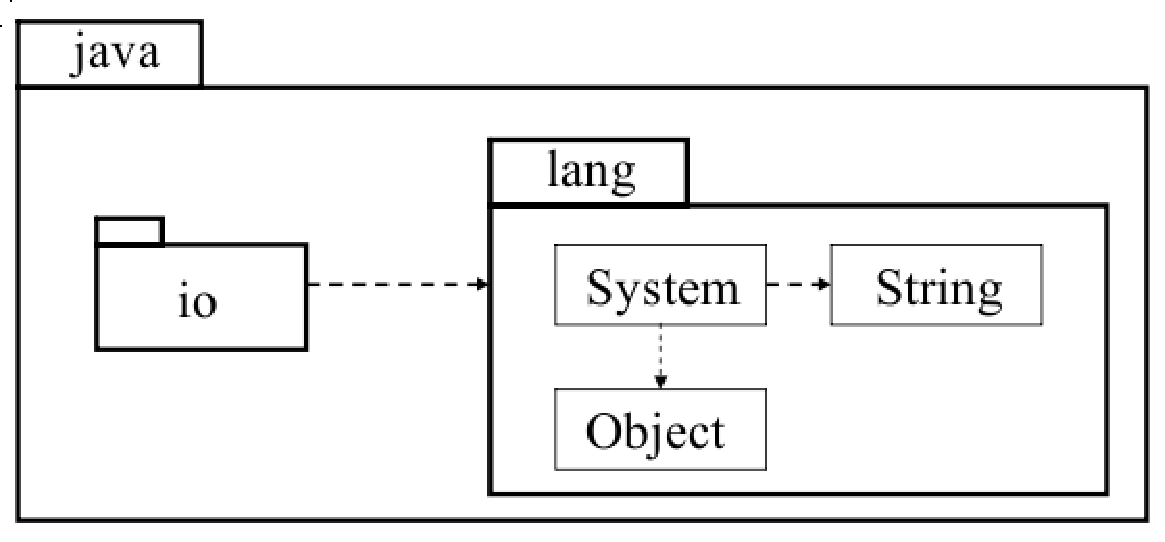
\includegraphics[width=0.6\textwidth]{images/Advanced-object-oriented-programming-1/fig-java-package.pdf}
\caption{Java包}
\label{fig:java-package}
\end{figure}

\subsection{JDK常用包}

JDK API中的常用包如表所示。

\begin{table}[!htbp]
  \centering
  \caption{JDK API常用包}
  \label{tab:java-package-list}
  \begin{tabular}{|c|c|c|}
    \hline
    {\bf 包名} & {\bf 功能说明} & {\bf 包的含义}   \\
    \hline
    java.lang & Java语言程序设计的基础类 & language的简写\\
    \hline
    java.awt & 创建图形用户界面和绘制图形图像的相关类 & 抽象窗口工具集\\
    \hline
    java.util & 集合、日期、国际化、各种实用工具 & utility的简写\\
    \hline
    java.io & 可提供数据输入/输出相关功能的类 & input/output的简写\\
    \hline
    java.net & Java网络编程的相关功能类 & 网络\\
    \hline
    java.sql & 提供数据库操作的相关功能类 & 结构化查询语言的简写\\
    \hline
  \end{tabular}
\end{table}


\subsection{包的创建}

package语句作为Java源文件的第一条语句,指明该文件中定义的类所在的包(若缺省该语句,则指定为无名包)。语法格式如下:

\begin{javaCode}
  package pkg1[.pkg2[.pkg3...]];
\end{javaCode}

\samplecode{创建包}

\begin{javaCode}
  package p1;
  public class Test {
    public void m1() {
      System.out.println("In class Test, method m1 is running!");
    }
  }
\end{javaCode}

package语句对所在源文件中定义的所有类型(包括接口、枚举、注解)均起作用。

Java编译器把包对应于文件系统的目录管理,package语句中,用“.”来指明包(目录)的层次。如果在程序Test.java中已定义了包p1,编译时采用如下方式:

\begin{shCode}
  > javac Test.java
\end{shCode}

则编译器会在当前目录下生成Test.class文件。

若在命令行下使用如下命令:

\begin{shCode}
  > java -d /home/xiaodong/work01 Test.java
\end{shCode}

“-d /home/xiaodong/work01”是传给Java编译器的参数,用于指定此次编译生成的.class文件保存到
该指定路径下,并且如果源文件中有package语句,则编译时会自动在目标路径下创建与包同名的目
录p1,再将生成的Test.class文件保存到该目录下。

\subsection{导入包中的类}

为使用定义在不同包中的Java类,需用import语句来引入所需要的类。语法格式:

\begin{javaCode}
  import pkg1[.pkg2...].(classname|*);  
\end{javaCode}

\samplecode{导入和使用有名包中的类}

\begin{javaCode}
  import p1.Test; //or import p1.*;
  public class TestPackage{
    public static void main(String args[]){
      Test t = new Test();
      t.m1();
    }
  }
\end{javaCode}

\subsection{Java包特性}

一个类如果未声明为public的,则只能在其所在包中被使用,其他包中的类即使
在源文件中使用import语句也无法引入它。可以不在源文件开头使用import语句
导入要使用的有名包中的类,而是在程序代码中每次用到该类时都给出其完整的
包层次,例如:

\begin{javaCode}
  public class TestPackage{ 
    public static void main(String args[]){ 
      p1.Test t = new p1.Test(); 
      t.m1(); 
    } 
  }
\end{javaCode}

%%%%%%%%%%%%%%%%%%%%%%%%%%%%%%%%%%%%%%%%%%%%%%%%%%%%%%%%%%%%%%
\section{继承}

\subsection{继承的概念}

继承(Inheritance)是面向对象编程的核心机制之一,其本质是在已有类型基础
之上进行扩充或改造,得到新的数据类型,以满足新的需要。

根据需要定义Java类描述“人”和“学生”信息,示例代码如下:

\samplecode{Class Person}
\begin{javaCode}
  public class Person {
    public String name;
    public int age;
    public Date birthDate;
    public String getInfo() {...}
  }
\end{javaCode}

\samplecode{Class Student}

\begin{javaCode}
  public class Student {
    public String name;
    public int age;
    public Date birthDate;
    public String school;
    public String getInfo() {...}
  }
\end{javaCode}

我们可以通过继承简化Student类的定义:

\samplecode{Class Student extends Person}

\begin{javaCode}
  public class Student extends Person {
    public String school;
  }
\end{javaCode}

Java类声明的语法格式如下:

\begin{javaCode}
  [< 修饰符 >] class < 类名 > [extends < 父类名 >] {
    [< 属性声明 >]
    [< 构造方法声明 >]
    [< 方法声明 >]
  }
\end{javaCode}

Object类是所有Java类的最高层父类,如果在类的声明中未使用extends关键字指明其父类,则默认父类为Object类。

Java只支持单继承,不允许多重继承。即:

\begin{itemize}
\item 一个子类只能有一个父类;
\item 一个父类可以派生出多个子类。
\end{itemize}

\begin{figure}[htb]
\centering
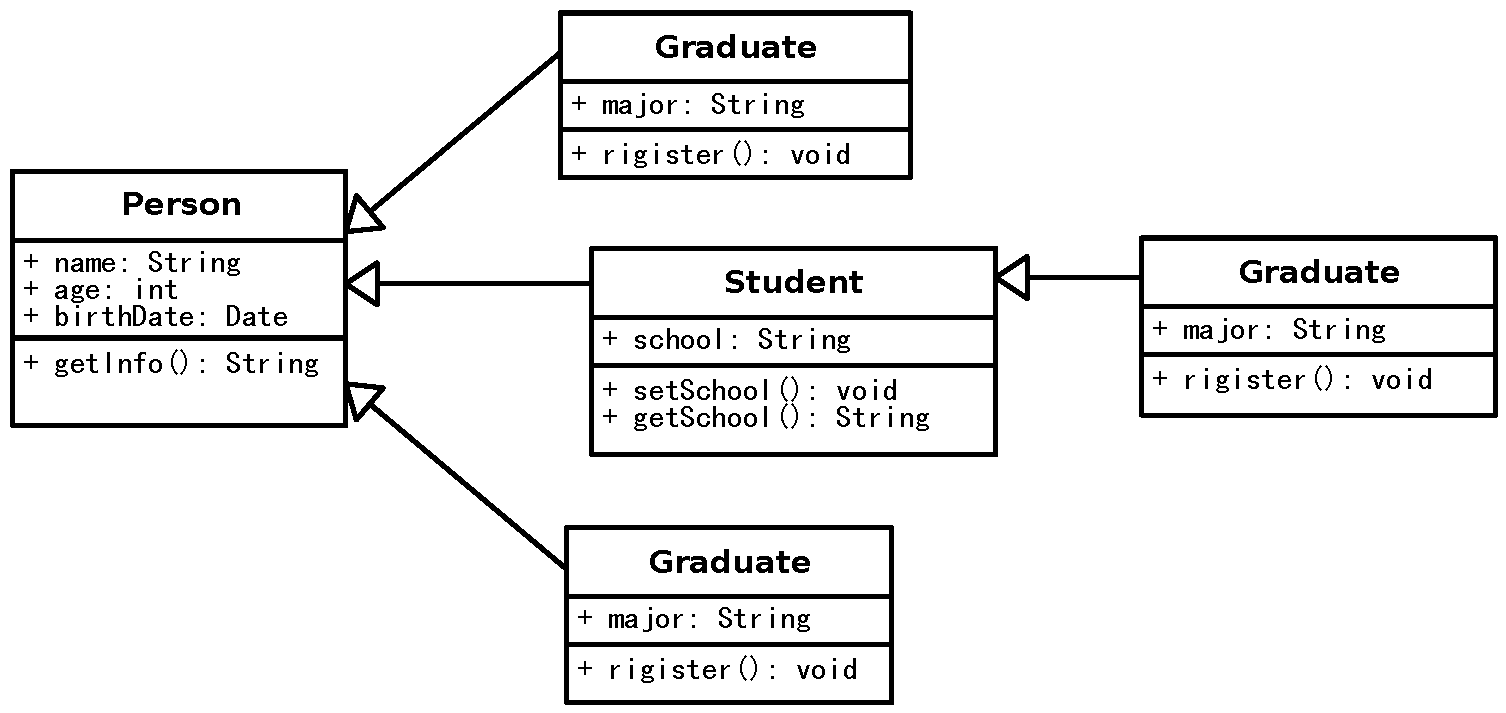
\includegraphics[width=0.9\textwidth]{images/Advanced-object-oriented-programming-1/fig-java-extends.pdf}
\caption{Java包}
\label{fig:java-package}
\end{figure}

\subsection{类之间的关系}

\begin{description}
\item[依赖关系] 一个类的方法中使用到另一个类的对象
  (uses-a)\footnote{车能够装载货物,车的装载功能(load()方法)对货物
    (goods)有依赖。}。
\item[聚合关系] 一个类的对象包含(通过属性引用)了另一个类的对象
  (has-a)\footnote{车有发动机、车轮等,Car对象是由Engine等对象构成
    的。}。
\item[泛化关系] 一般化关系(is-a),表示类之间的继承关系、类和接口之间
  的实现关系以及接口之间的继承关系。
\end{description}

\section{访问控制}

访问控制是指对Java类或类中成员的操作进行限制,即规定其在多大的范围内可以被直接访问。

\subsection{类的访问控制}

在声明Java类时可以在class关键字前使用public来修饰,也可以不使用该修饰
符。public的类可在任意场合被引入和使用,而非public的类只能在其所在包中
被使用。

\subsection{类中成员的访问控制}

\begin{table}[!htbp]
  \centering
  \caption{类成员的访问控制}
  \label{tab:java-class-member-access-control}
  \begin{tabular}{|c|c|c|c|c|}
    \hline
    {\bf 修饰符/作用范围} & {\bf 同一个类} & {\bf 同一个包} & {\bf 子类} & {\bf 任何地方} \\
    \hline
    public & yes & yes & yes & yes\\
    \hline
    protected  & yes & yes & yes & no \\
    \hline
    无修饰符 & yes & yes & no & no \\
    \hline
    private & yes & no & no & no \\
    \hline
  \end{tabular}
\end{table}

\subsection{访问控制注意的一些问题}

\begin{itemize}
\item 一般不提倡将属性声明为public的,而构造方法和需要外界直接调用的普通方法则适合声明为
  public的。
\item 在位于不同的包内,必须是子类的对象才可以直接访问其父类的protected成员,而父类自身
  的对象反而不能访问其所在类中声明的protected成员。
\item 所谓“访问控制”只是控制对Java类或类中成员的直接访问,而间接访问是不做控制的,也不该
  进行控制。
\end{itemize}

\begin{figure}[htb]
\centering
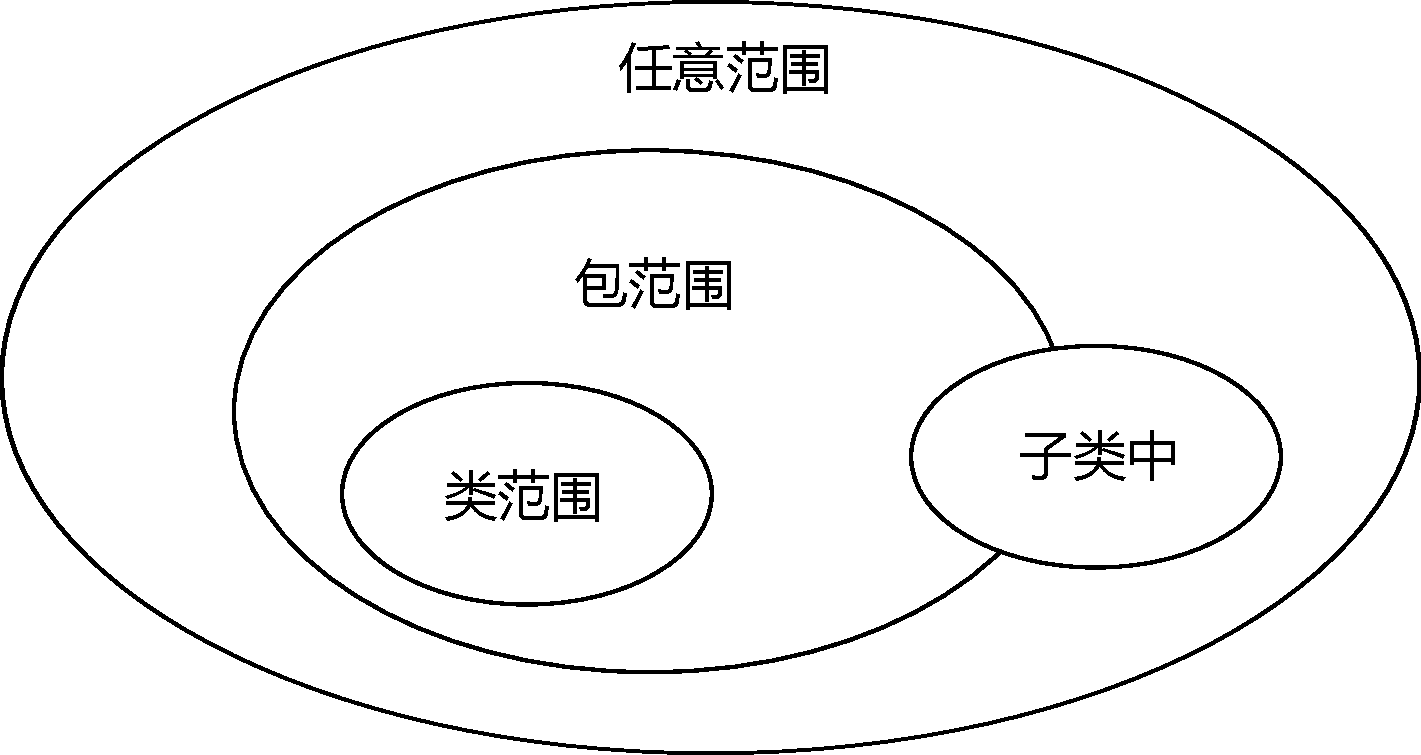
\includegraphics[width=0.6\textwidth]{images/Advanced-object-oriented-programming-1/fig-java-access-control.pdf}
\caption{Java访问控制}
\label{fig:java-access-control}
\end{figure}


\subsection{访问控制protected}

\samplecode{A.java}

\begin{javaCode}
  package p1;
  public class A {
    public int m = 5;
    protected int n = 6;
  }
\end{javaCode}

\samplecode{B.java}
\begin{javaCode}
  package p2;
  import p1.A;
  public class B extends A {
    public void mb() {
      m = m + 1;
      n = n * 2;
    }
    
    public static void main(String[] args) {
      B b = new B();
      b.m = 7;  // 合法
      b.n = 8;   // 合法
      A a = new A();
      a.m = 9 // 合法
      a.n = 10 // 非法
    }
  }
\end{javaCode}

\section{同名问题}

\subsection{方法重写}

在子类中可以根据需要对从父类中继承来的方法进行重新定义,此称方法重写(Override)或覆盖。

\begin{itemize}
\item 重写方法必须和被重写方法具有相同的方法名称、参数列表和返回值类型;
\item 重写方法不能使用比被重写方法更严格的访问权限;
\item 重写方法不允许声明抛出比被重写方法范围更大的异常类型。
\end{itemize}

\samplecode{方法重写示例:Person.java}
\begin{javaCode}
  public class Person {
    String name;
    int age;
    public String getInfo() {
      return "Name:"+ name + "\t" +"age:"+ age;
    }
  }
\end{javaCode}

\samplecode{方法重写示例:Student.java}

\begin{javaCode}
  public class Student extends Person {
    private String school;
    public void setSchool(String scholl) {
      this.school = school;
    }
    public String getSchool(){
      return school;
    }
    public String getInfo() {
      return "Name:"+ name + "\tAge:"+ age + "\tSchool:" + school;
    }
  }
\end{javaCode}

\samplecode{方法重写示例:Parent.java}
\begin{javaCode}
  public class Parent {
    public void method1() {...}
  }
\end{javaCode}

\samplecode{方法重写示例:Child.java}

\begin{javaCode}
  public class Child extends Parent {
    private void method1() {} //非法,权限更严格
  }
\end{javaCode}

\subsection{同名属性}

\begin{javaCode}
  public class Person {
    int age = 5;
    public int getAge() {
      return age;
    }
    public int getInfo() {
      return age;
    }
  }
\end{javaCode}

\begin{javaCode}
  public class Student extends Person {
    int age = 6;
    public int getAge() {
      return age;
    }
  }
\end{javaCode}

\begin{javaCode}
  public class Test {
    public static void main(String args[]) {
      Person p = new Person();
      System.out.println(p.getAge());
      Student s = new Student();
      System.out.println(s.age);
      System.out.println(s.getAge());
      System.out.println(s.getInfo());
    }
  }
\end{javaCode}

上述程序的输出结果为:

\begin{stdoutCode}
  5
  6
  6
  5
\end{stdoutCode}

\descript{对上述Student对象同名属性的几点说明}

\begin{enumerate}
\item 以“对象名.属性名”方式直接访问时,使用的是子类中添加的属性age;
\item 调用子类添加或者重写的方法时,方法中使用的是子类定义的属性age;
\item 调用父类中定义的方法时,方法中使用的是父类中的属性age;
\item 可以理解为“{\bf\Blue 层次优先~就近原则}”,在哪个层次中的代码,就优先使用该层次类中
  定义的属性。不提倡使用同名属性。
\end{enumerate}

\subsection{关键字super} 

在存在命名冲突(子类中存在方法重写或添加同名属性)的情况下,子类中的代码将自动使用子类中
的同名属性或重写后的方法。当然也可以在子类中{\Red 使用关键字super引用父类中的成分}:

\subsubsection{访问父类中定义的属性}

\begin{javaCode}
  super.<属性名>  
\end{javaCode}

\subsubsection{调用父类中定义的成员方法}

\begin{javaCode}
  super.<方法名>(<实参列表>)
\end{javaCode}

\subsubsection{子类构造方法中调用父类的构造方法}

\begin{javaCode}
  super(<实参列表>)  
\end{javaCode}

super的追溯不仅限于直接父类,而是先从直接父类开始查找,如果找不到则逐层
上溯,一旦在某个层次父类中找到匹配成员即停止追溯并使用该成员。

\samplecode{super用法示例A}

\begin{javaCode}
  class Animal {
    protected int i = 1;   //用于测试同名属性,无现实含义
  }

  class Person extends Animal {
    protected int i = 2;     //用于测试同名属性,无现实含义
    private String name = "Tom";
    private int age = 9;
    public String getInfo() {
      return "Name:" + name + "\tAge:" + age;
    }
    public void testI() {
      System.out.println(super.i);
      System.out.println(i);
    }
  }
\end{javaCode}

\samplecode{super用法示例B}

\begin{javaCode}
  class Student extends Person {
    private int i = 3;
    private String school = "THU";
    public String getInfo() {       //重写方法
      return super.getInfo() + "\tSchool:" + school;
    }
    public void testI() {       //重写方法
      System.out.println(super.i);
      System.out.println(i);
    }
  }
  public class Test {
    public static void main(String args[]) {
      Person p = new Person();
      System.out.println(p.getInfo());
      p.testI();
      Student s = new Student();
      System.out.println(s.getInfo());
      s.testI();
    }
  }
\end{javaCode}

上述代码的输出结果为:

\begin{stdoutCode}
  Name:Tom Age:9
  1
  2
  Name:Tom Age:9 School:THU
  2
  3  
\end{stdoutCode}

\subsection{关键字this}

在Java方法中,不但可以直接使用方法的局部变量,也可以使用调用该方法的对
象。为解决可能出现的命名冲突,Java语言引入this关键字来标明方法的当前对
象。分为两种情况:

\begin{itemize}
\item 在普通方法中,关键字this代表方法的调用者,即本次调用了该方法的对象;
\item 在构造方法中,关键字this代表该方法本次运行所创建的那个新对象。
\end{itemize}

this作为一个特殊的引用类型变量,可以通过“{\Red this.成员}”的方式访问
其引用的当前对象的属性和方法。

\samplecode{this用法示例}
\begin{javaCode}
  public class MyDate {
    private int day = 17;
    private int month = 2;

    public MyDate(int day, int month) {
      this.day = day; // A
      this.month = month;
    }
    ... // Some methods 

    public void setAll(int day, int month) {
      this.setMonth(month); // B
      this.setDay(day);
    }
  }
\end{javaCode}

\descript{关于this的归纳说明}

\begin{enumerate}
\item 在Java方法中直接给出变量名而不是“对象名.变量名”的方式访问一个变
  量,系统首先尝试作为局部变量来处理;如果方法中不存在该名字的局部变量,
  才会到方法当前对象的成员变量中查找。
\item 在Java方法中直接调用一个方法而不指定其调用者时,则默认调用者为当
  前对象this。
\end{enumerate}

\newpage
\section*{实验设计}
\sline

%% Week 03 %%
\chapter{Java 面向对象编程进阶 B}
\label{chp:Advanced-object-oriented-programming-2}

\section*{基本信息}
\sline
\begin{description}
\item[课程名称:] Java应用与开发
\item[授课教师:] 王晓东
\item[授课时间:] 第二周(根据校历,本周有两次课)
\item[参考教材:] 本课程参考教材及资料如下:
  \begin{itemize}
  \item 陈国君主编,Java程序设计基础(第5版),清华大学出版社,2015.5
  \item Bruce Eckel, Thinking in Java (3rd)
  \end{itemize}
\end{description}

\section*{教学目标}

\sline

\begin{enumerate}
\item 理解多态和虚方法调用的概念,掌握其用法
\item 掌握方法重载的方法
\item 掌握static属性、方法和初始化块的用法
\item 了解设计模式,掌握单例设计模式
\item 掌握final关键字的概念和使用方法
\end{enumerate}  

\section*{授课方式}

\sline
\begin{description}
\item[理论课:] 多媒体教学、程序演示
\item[实验课:] 上机编程
\end{description}

\newpage
\section*{教学内容}
\sline

%%%%%%%%%%%%%%%%%%%%%%%%%%%%%%%%%%%%%%%%%%%%%%%%%%%%%%%%%%%%%%
\section{多态性}

\subsection{多态的概念}

在Java中,子类的对象可以替代父类的对象使用称为{\hei 多态}。Java引用变量
与所引用对象间的类型匹配关系如下:

\begin{itemize}
\item 一个对象只能属于一种确定的数据类型,该类型自对象创建直至销毁不能
  改变。
\item 一个引用类型变量可能引用(指向)多种不同类型的对象——既可以引用其
  声明类型的对象,也可以引用其声明类型的子类的对象。
  \begin{javaCode}
    Person p = new Student(); //Student 是 Person 的子类  
  \end{javaCode}
\end{itemize}

\begin{figure}[htb]
  \centering
  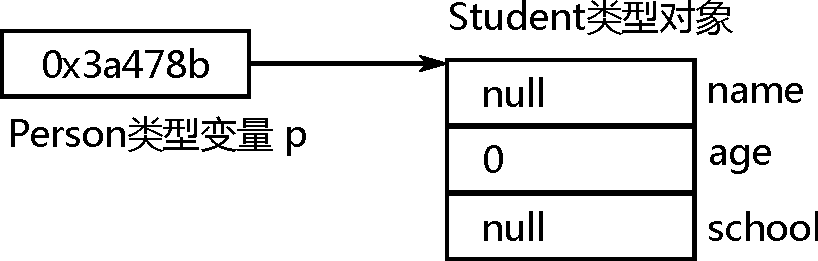
\includegraphics[width=0.6\textwidth]{images/Advanced-object-oriented-programming-2/fig-poly.pdf}
  \caption{Java多态}
  \label{fig:poly}
\end{figure}

多态性同样适用与引用类型数组元素。

\begin{javaCode}
  Person[] p = new Person[3]; 
  p[0] = new Student(); // 假设 Student 类继承了 Person 类
  p[1] = new Person();
  p[2] = new Graduate(); //假设 Graduate 类继承了 Student 类
\end{javaCode}

一个引用类型变量如果声明为父类的类型,但实际引用的是子类对象,该变量则不能再访问子类
中添加的属性和方法,这体现了父类引用对子类对象的能力屏蔽性。

\begin{javaCode}
  Student m = new Student();
  m.setSchool("ouc"); // 合法
  Person e = new Student();
  e.setSchool("ouc"); // 非法
\end{javaCode}

\subsection{多态用法示例}

\samp{Person.java}

\begin{javaCode}
  public class Person {...}
\end{javaCode}

\samp{Student.java}

\begin{javaCode}
  public class Student extends Person {
    private String school;

    public void setSchool(String school) {
      this.school = school;
    }

    public String getSchool() {
      return school;
    }

    @Override
    public String getInfo() {
      return super.getInfo() + "\tSchool: " + school;
    }
  }
\end{javaCode}

\samp{PolymorphismSample.java}

\begin{javaCode}
  public class PolymorphismSample {
    public void show(Person p) {
      System.out.println(p.getInfo());
    }
    
    public static void main(String[] args) {
      PolymorphismSample ps = new PolymorphismSample();
      Person p = new Person();
      ps.show(p);
      Student s = new Student();
      ps.show(s);
    }
  }
\end{javaCode}

\notice{多态提升方法通用性}

以上代码中,show()方法既可以处理Person类型的数据,又可以处理Student类型
的数据,乃至未来定义的任何Person子类类型的数据,即不必为相关的每种类型
单独声明一个处理方法,提高了代码的通用性。

\subsection{虚方法调用}

思考:一个引用类型的变量如果声明为父类的类型,但实际引用的是子类对象,
则该变量就不能再访问子类中添加的属性和方法。但如果此时调用的是父类中声
明过、且在子类中重写过的方法,情况如何?

补充代码。

\subsection{对象造型}

引用类型数据值之间的强制类型转换称为{\hei 造型(Casting)}。造型以下几种情况需要注意:

\begin{enumerate}
\item 从子类到父类的类型转换可以自动进行。
  \begin{javaCode}
    Person p = new Student();    
  \end{javaCode}
\item 在多态的情况下,有时我们可能需要恢复一个对象的本来面目,以发挥其
  全部潜力。从父类到子类的类型转换必须通过造型实现。
  \begin{javaCode}
    Person p1 = new Student();  
    Student s1 = (Student)p1;   // 合法
    Person p2 = new Person();   
    Student s2 = (Student)p2;  // 非法  
  \end{javaCode}
\item 无继承关系的引用类型间的转换是非法的。
  \begin{javaCode}
    String s = "Hello World!";
    Person p = (Person)s; // 非法  
  \end{javaCode}
\end{enumerate}

\subsection{instanceof运算符}

如果运算符instanceof左侧的变量当前时刻所引用的对象的{\hei\Red 真正类型}是
其右侧给出的类型{\Blue 或者是其子类},则整个表达式的结果为true。

\begin{javaCode}
class Person { --- }
class Student extends Person { --- }

public class Tool {
  public void distribute(Person p) {
    if (p instanceof Student) {
      System.out.println("处理 Student 类型及其子类类型对象");
    } else {
      System.out.println("处理 Person 类型及其子类类型对象");
    }
  }
}
\end{javaCode}

\begin{javaCode}
public class Test() {
  public static void main(String[] args) {
    Tool t = new Tool();
    Student s = new Student();
    t.distribute(t);
  }
}
\end{javaCode}

\subsection{虚方法调用和造型}

\codeset{package sample.oop.poly}

\begin{itemize}\small
\item VirtualMethodSample.java
\item Person.java
\item Student.java
\end{itemize}
  
强调以下与虚方法调用和造型相关的重点:
  
\begin{itemize}
\item 系统根据运行时对象的真正类型来确定具体调用哪一个方法,这一机制被称为
  {\hei\Blue 虚方法调用}。
\item 造型是引用类型数据值之间的强制类型转换。
\item instanceof运算符判断的是当前所引用对象的真正类型是什么,而不是声明的引用类型。
\end{itemize}

\section{方法重载}

\subsection{方法重载的概念}

在一个类中存在多个同名方法的情况称为{\hei 方法重载(Overload)}。Java对方法重载有以下要求:

\begin{itemize}
\item 重载方法参数列表必须不同。
\item 重载既可以用于普通方法,也可以用于构造方法。
\end{itemize}

\codeset{sample.oop.MethodOverloadSample.java}


\subsection{调用重载的构造方法}
  
\subsubsection{使用this调用当前类中重载构造方法}

可以在构造方法的第一行使用关键字this调用其它(重载的)构造方法。

\begin{javaCode}
  public class Person {
    ...
    public Person(String name,int age) {
      this.name = name;
      this.age = age;
    }
    public Person(String name) {
      this(name, 18);
    }
    ...
  }
\end{javaCode}

\notice{注意}

关键字this的此种用法只能用在构造方法中,且this()语句如果出
现必须位于方法体中代码的第一行。

\subsubsection{使用super调用父类构造方法}

\samp{Person.java}

\begin{javaCode}
  public class Person {
    ... (此处没有无参构造方法)
    public Person(String name, int age) {
      this.name = name;
      this.age = age;
    }
    ...
  }  
\end{javaCode}

\samp{Student.java}

\begin{javaCode}
  public class Student extends Person {
    private String school;
    public Student(String name, int age, String school) {
      super(name, age); // 显式调用父类有参构造方法
      this.school = school;
    }
    public Student(String school) { //编译出错
      // super(); // 隐式调用父类有参构造方法,则自动调用父类无参构造方法
      this.school = school;
    }
  }
\end{javaCode}

\notice{上述代码为什么会编译出错?}

{\Blue\hei 在Java类的构造方法中一定直接或间接地调用了其父类的构造方法(Object类除外)。}

\begin{enumerate}
\item 在子类的构造方法中可使用super语句调用父类的构造方法,其格式为super(<实参列表>)。
\item 如果子类的构造方法中既没有显式地调用父类构造方法,也没有使用this关键字调用同一个类
  的其他重载构造方法,则系统会默认调用父类无参数的构造方法,其格式为super()。
\item 如果子类构造方法中既未显式调用父类构造方法,而父类中又没有无参的构造方法,则编译出
  错。
\end{enumerate}

\codeset{sample.oop.ConstructorOverloadSample.java}
  


\subsection{对象构造/初始化细节}

\begin{description}
\item [第一阶段] 为新建对象的实例变量分配存储空间并进行默认初始化。
\item [第二阶段] 按下述步骤继续初始化实例变量:
  \begin{enumerate}
  \item 绑定构造方法参数;
  \item 如有this()调用,则调用相应的重载构造方法然后跳转到步骤5;
  \item 显式或隐式追溯调用父类的构造方法(Object类除外);
  \item 进行实例变量的显式初始化操作;
  \item 执行当前构造方法的方法体中其余的语句。 
  \end{enumerate}
\end{description}

\section{关键字static}

在Java类中声明{\hei\Red 属性、方法和内部类}时,可使用关键字static作为修饰符。

\begin{itemize}
\item static标记的属性或方法由整个类(所有实例)共享,如访问控制权限
  允许,可不必创建该类对象而直接用类名加“.”调用。
\item static成员也称{\hei\Blue “类成员”或“静态成员”},如“类属
  性”、“类变量”、“类方法”和“静态方法”等。
\end{itemize}

\subsection{static属性和方法}

\subsubsection{static属性}

\begin{itemize}
\item static属性由其所在类(包括该类所有的实例)共享。
\item 非static属性则必须依赖具体/特定的对象(实例)而存在。
\end{itemize}

\subsubsection{static方法}

要在static方法中调用其所在类的非static成员,应首先创建一个该类的对象,
通过该对象来访问其非static成员。

\codeset{sample.oop.StaticMemberAndMethodSample.java}


\subsection{初始化块}

\subsubsection{static初始化块}

在类的定义体中,方法的外部可包含static语句块,{\Red static块仅在其所属
  的类被载入时执行一次},通常用于初始化化static(类)属性。

\subsubsection{非static初始化块}

非static的初始化块在创建对象时被自动调用。

\codeset{sample.oop.StaticInitBlockSample.java}

\subsection{静态导入}

静态导入用于在一个类中导入其他类或接口中的static成员,语法格式如下:

\begin{javaCode}
  import static <包路径>.<类名>.*

  import static <包路径>.<类名>.<静态成员名>
\end{javaCode}

\samp{静态导入应用示例}

\begin{javaCode}
import static java.lang.Math.*;
public class Test {
  public static void main(String[] args) {
    double d = sin(PI * 0.45);
    System.out.println(d);
  }
}
\end{javaCode}

\subsection{Singleton设计模式}

所谓“模式”就是被验证为有效的常规问题的典型解决方案。{\hei 设计模式
  (Design Pattern)}在面向对象分析设计和软件开发中占有重要地位。好的设
计模式可以使我们更加方便的重用已有的成功设计和体系结构,极大的提高代码
的重用性和可维护性。

经典设计模式分类主要分为以下三大类:

\begin{description}
\item[创建型模式] 涉及对象的实例化,特点是不让用户代码依赖于对象的创建或排列方式,避免用户直接使用new创建对象。\\
  {\Red\kai 工厂方法模式、抽象工厂方法模式、生成器模式、原型模式和单例
    模式}
\item[行为型模式] 涉及怎样合理的设计对象之间的交互通信,以及合理为对象分配职责,让设计富有弹性、易维护、易复用。\\
  {\Blue\kai 责任链模式、命令模式、解释器模式、迭代器模式、中介者模式、
    备忘录模式、观察者模式、状态模式、策略模式、模板方法模式和访问者模
    式}
\item[结构型模式] 涉及如何组合类和对象以形成更大的结构,和类有关的结构型模式涉及如何合理使用继承机制,和对象有关的结构型模式涉及如何合理的使用对象组合机制。\\
  {\Mage\kai 适配器模式、组合模式、代理模式、享元模式、外观模式、桥接模
    式和装饰模式}
\end{description}


Singleton设计模式也称“单子模式”或“单例模式”。

\notice{采用调试方式讲解示例代码}

Singleton代码的特点包括以下几个方面:

\begin{enumerate}
\item 使用静态属性onlyone来引用一个“全局性”的Single实例。
\item 将构造方法设置为private的,这样在外界将不能再使用new关键字来创建该类的新实例。
\item 提供public static的方法getSingle()以使外界能够获取该类的实例,达到全局可见的效果。
\end{enumerate}

在任何使用到Single类的Java程序中(这里指的是一次运行中),需要确保只有
一个Single类的实例存在(如Web应用ServletContext全局上下文对象),则使用
该模式。

\section{关键字final}

在声明Java类、变量和方法时可以使用关键字final来修饰,以使其具有“终态”的特性:

\begin{enumerate}\kai
\item final标记的类不能被继承;
\item final标记的方法不能被子类重写;
\item final标记的变量(成员变量或局部变量)即成为常量,只能赋值一次;
\item final标记的成员变量必须在声明的同时或在每个构造方法中显式赋值,然后才能使用;
\item final不允许用于修饰构造方法、抽象类以及抽象方法。
\end{enumerate}

关键字final应用举例如下:

\begin{javaCode}
public final class Test {
  public static int totalNumber = 5;
  public final int id;
  public Test() {
    id = ++totalNumber; // 赋值一次
  }
  public static void main(String[] args) {
    Test t = new Test();
    System.out.println(t.id);
    final int i = 10;
    final int j;
    j = 20;
    j = 30;  // 非法
  }
}
\end{javaCode}

\section{课后习题}

\tta{简答题}
\begin{enumerate}
\item 为什么建议Java类需要编写无参构造方法,哪怕该方法什么都没做?
\item 关键字static都可以用来修饰Java类的那些成员?
\end{enumerate}

\tta{小编程}
\begin{enumerate}
\item 练习本节中所有示例代码,理解并掌握其用法。
\item 自行调试单例设计模式程序,学习Eclipse的Debug方法,练习断点、单
  步执行、跟进方法等操作,查看内存变化。
\end{enumerate}
\chapter{Java内存模型与分配机制}
\label{chp:Java-memory-allocation}

\section*{基本信息}
\sline
\begin{description}
\item[课程名称:] Java应用与开发
\item[授课教师:] 王晓东
\item[授课时间:] 第二周(根据校历,本周有两次课)
\item[参考教材:] 本课程参考教材及资料如下:
  \begin{itemize}
  \item 陈国君主编,Java程序设计基础(第5版),清华大学出版社,2015.5
  \item Bruce Eckel, Thinking in Java (3rd)
  \end{itemize}
\end{description}

\section*{教学目标}

\sline

\begin{enumerate}
\item 理解JVM内存模型,掌握JVM内存构成
\item 理解Java程序的运行过程,学会通过调试模式观察内存的变化
\item 了解Java内存管理,认识垃圾回收
\item 建立编程时高效利用内存、避免内存溢出的理念
\end{enumerate}  

\section*{授课方式}

\sline
\begin{description}
\item[理论课:] 多媒体教学、程序演示
\item[实验课:] 上机编程
\end{description}

\newpage
\section*{教学内容}
\sline

%%%%%%%%%%%%%%%%%%%%%%%%%%%%%%%%%%%%%%%%%%%%%%%%%%%%%%%%%%%%%%
\section{Java内存模型}

\subsection{Java虚拟机(Java Virtual Machine, JVM)}

Java虚拟机的架构如图\ref{fig:jvm-arch}所示。

\begin{figure}[htb]
  \centering
  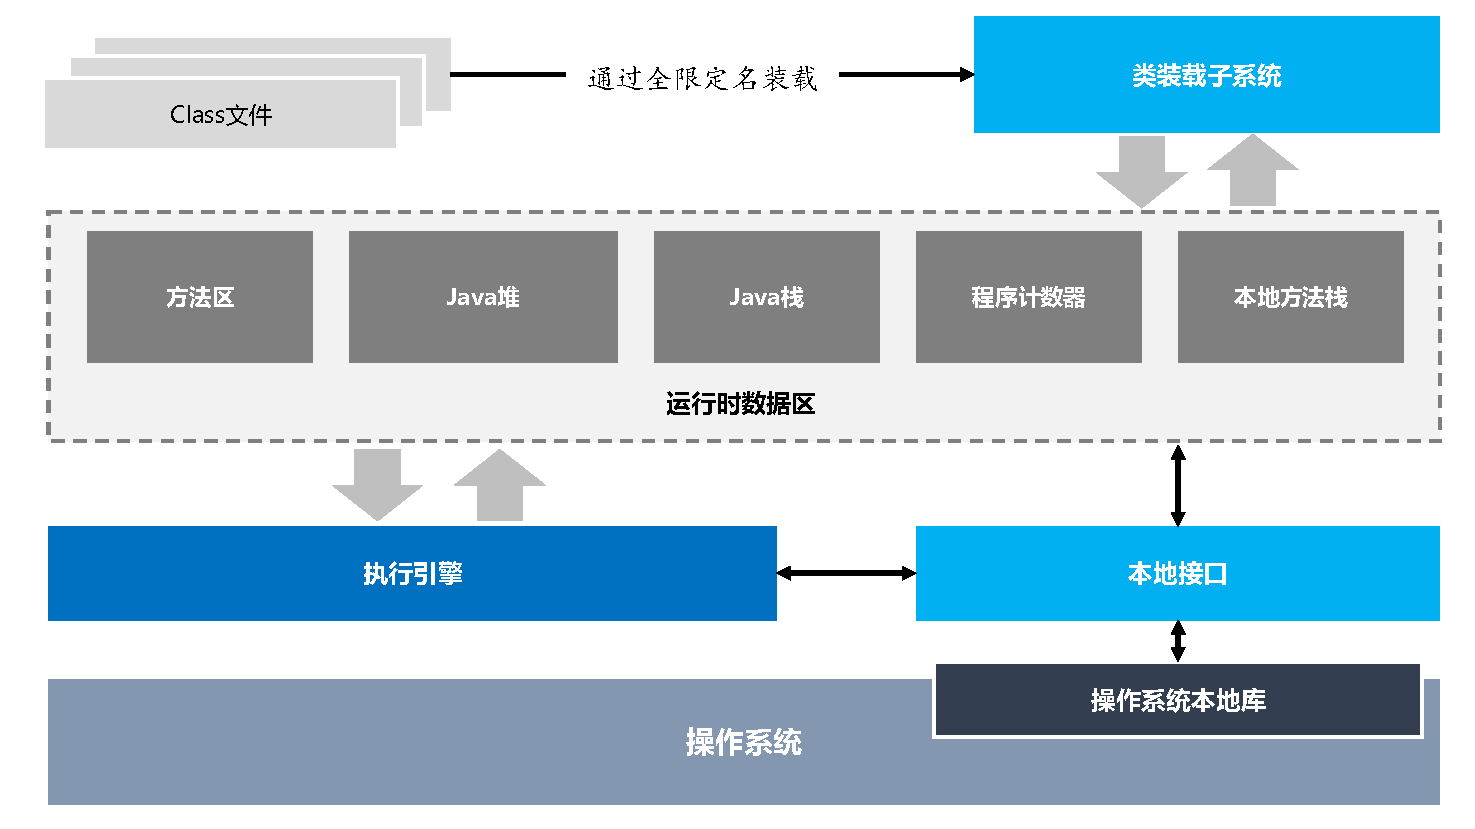
\includegraphics[width=\textwidth]{images/Java-memory-allocation/fig-jvm-arch.pdf}
  \caption{Java虚拟机架构}
  \label{fig:jvm-arch}
\end{figure}

\begin{itemize}
\item Java程序运行在JVM上,JVM是程序与操作系统之间的桥梁。
\item JVM实现了Java的平台无关性。
\item JVM是内存分配的前提。
\end{itemize}

\subsection{JVM内存模型}

\begin{figure}[htb]
  \centering
  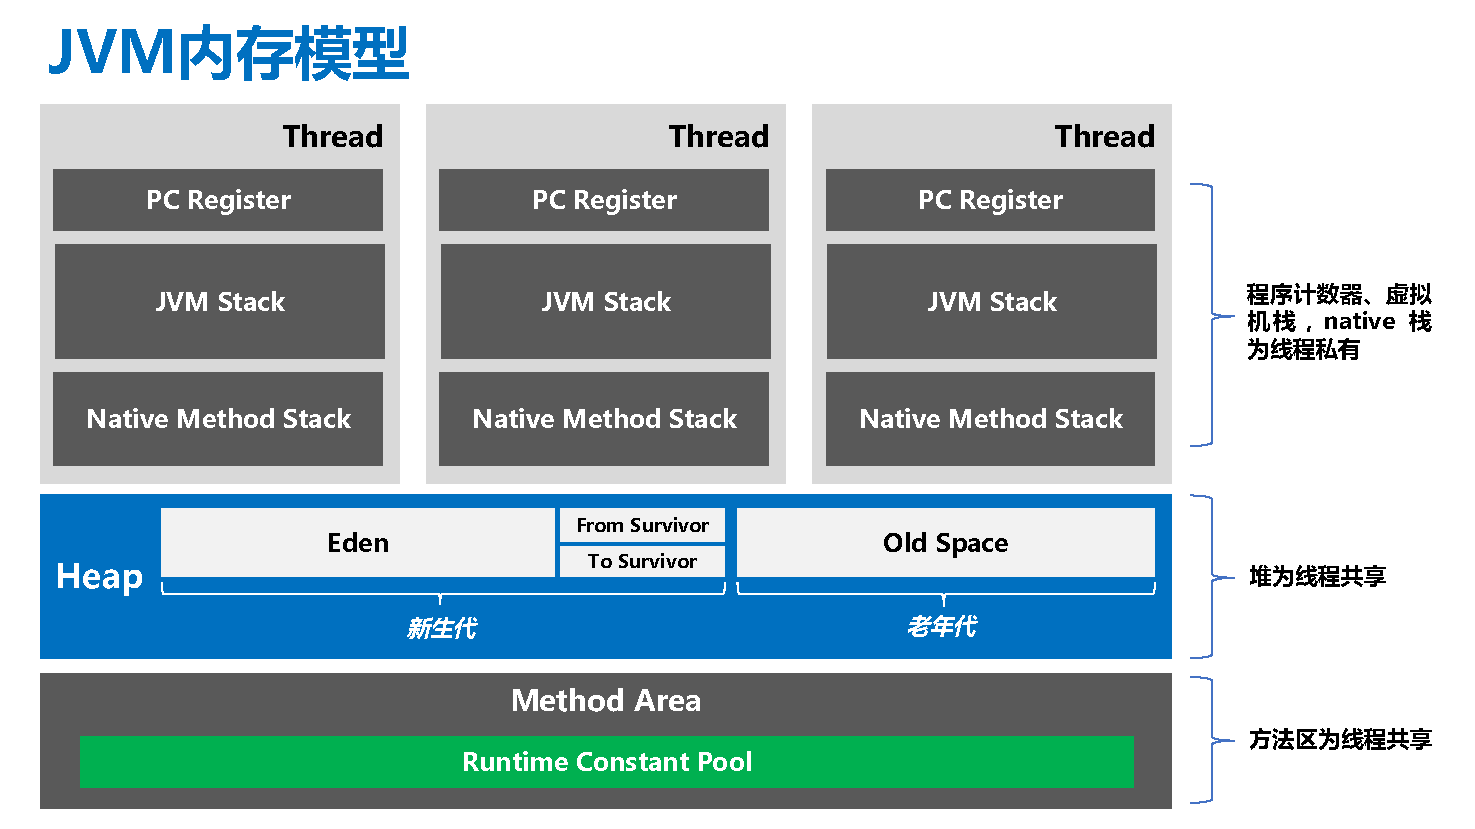
\includegraphics[width=\textwidth]{images/Java-memory-allocation/fig-java-memory-arch.pdf}
  \caption{JVM内存模型}
  \label{fig:java-memory-arch}
\end{figure}

Java程序运行过程会涉及的内存区域包括:

\begin{description}
\item[程序计数器] 当前线程执行的字节码的行号指示器。
\item[栈] 保存局部变量的值,包括:用来保存基本数据类型的值;保存类的实
  例,即堆区对象的引用(指针),也可以用来保存加载方法时的帧。(Stack)
\item[堆] 用来存放动态产生的数据,如new出来的对象和数组\footnote{注意创
    建出来的对象只包含属于各自的成员变量,并不包括成员方法。因为同一个
    类的对象拥有各自的成员变量,存储在各自的堆内存中,但是他们共享该类
    的方法,并不是每创建一个对象就把成员方法复制一次。}。(Heap)
\item[常量池] JVM为每个已加载的类型维护一个常量池,常量池就是这个类型用
  到的常量的一个有序集合。包括直接常量(基本类型、String)和对其他类型、
  方法、字段的符号引用。池中的数据和数组一样通过索引访问,常量池
  在Java程序的动态链接中起了核心作用。(Perm)
\item[代码段] 存放从硬盘上读取的源程序代码。(Perm)
\item[数据段] 存放static定义的静态成员。{\Red (Perm)} 
\end{description}

\section{Java程序内存运行分析}

\subsection{预备知识和所用讲解程序}

\begin{enumerate}
\item 一个Java文件,只要有main入口方法,即可认为这是一个Java程序,可以
  单独编译运行。
\item 无论是普通类型的变量还是引用类型的变量(俗称实例),都可以作为局
  部变量,他们都可以出现在栈中。
\item 普通类型的变量在栈中直接保存它所对应的值,而引用类型的变量保存的
  是一个指向堆区的指针。通过这个指针,就可以找到这个实例在堆区对应的对
  象。因此,{\hei\Red 普通类型变量只在栈区占用一块内存,而引用类型变量
    要在栈区和堆区各占一块内存}。
\end{enumerate}

\samp{Test.java}

\begin{javaCode}
  public class Test {
    public static void main(String[] args) {
      Test test = new Test(); //1
      int data = 9; //2
      BirthDate d1 = new BirthDate(22, 12, 1982); //3
      BirthDate d2 = new BirthDate(10, 10, 1958); //4
      test.m1(data); //5
      test.m2(d1); //7
      test.m3(d2);
    }

    public void m1(int i) {
      i = 1234; //6
    }
    public void m2(BirthDate b) {
      b = new BirthDate(15, 6, 2010); //8
    }
    public void m3(BirthDate b) {
      b.setDay(18);
    }
  }
\end{javaCode}

\subsection{程序调用过程}

\subsubsection{程序调用过程(一)}

\begin{itemize}
\item JVM自动寻找main方法,执行第一句代码,创建一个Test类的实例,在栈中分配一块内存,存放
  一个指向堆区对象的指针110925。
\item 创建一个int型的变量data,由于是基本类型,直接在栈中存放data对应的值9。
\item 创建两个BirthDate类的实例d1、d2,在栈中分别存放了对应的指针指向各自的对象。它们在实
  例化时调用了有参数的构造方法,因此对象中有自定义初始值。
\end{itemize}

\subsubsection{程序调用过程(二)}

\begin{itemize}
\item 调用test对象的m1方法,以data为参数。JVM读取这段代码时,检测到i是局部变量,则会把i放
  在栈中,并且把data的值赋给i。
\end{itemize}

\subsubsection{程序调用过程(三)}

\begin{itemize}
\item 把1234赋值给i。
\end{itemize}

\subsubsection{程序调用过程(四)}

\begin{itemize}
\item m1方法执行完毕,立即释放局部变量i所占用的栈空间。
\end{itemize}

\subsubsection{程序调用过程(五)}

\begin{itemize}
\item 调用test对象的m2方法,以实例d1为参数。JVM检测到m2方法中的b参数为
  局部变量,立即加入到栈中,由于是引用类型的变量,所以b中保存的是d1中的
  指针,此时b和d1指向同一个堆中的对象。在b和d1之间传递是指针。
\end{itemize}

\subsubsection{程序调用过程(六)}

\begin{itemize}
\item m2方法中又实例化了一个BirthDate对象,并且赋给b。在内部执行过程是:
  在堆区new了一个对象,并且把该对象的指针保存在栈中b对应空间,此时实
  例b不再指向实例d1所指向的对象,但是实例d1所指向的对象并无变化,未
  对d1造成任何影响。
\end{itemize}

\subsubsection{程序调用过程(七)}

\begin{itemize}
\item m2方法执行完毕,立即释放局部引用变量b所占的栈空间,注意只是释放了
  栈空间,堆空间要等待自动回收。
\end{itemize}

\subsubsection{程序调用过程(八)}

\begin{itemize}
\item 调用test实例的m3方法,以实例d2为参数。JVM会在栈中为局部引用变
  量b分配空间,并且把d2中的指针存放在b中,此时d2和b指向同一个对象。再调
  用实例b的setDay方法,其实就是调用d2指向的对象的setDay方法。
\item 调用实例b的setDay方法会影响d2,因为二者指向的是同一个对象。
\item m3方法执行完毕,立即释放局部引用变量b。
\end{itemize}

\begin{figure}[htb]
  \begin{minipage}[t]{0.5\linewidth}
    \centering
    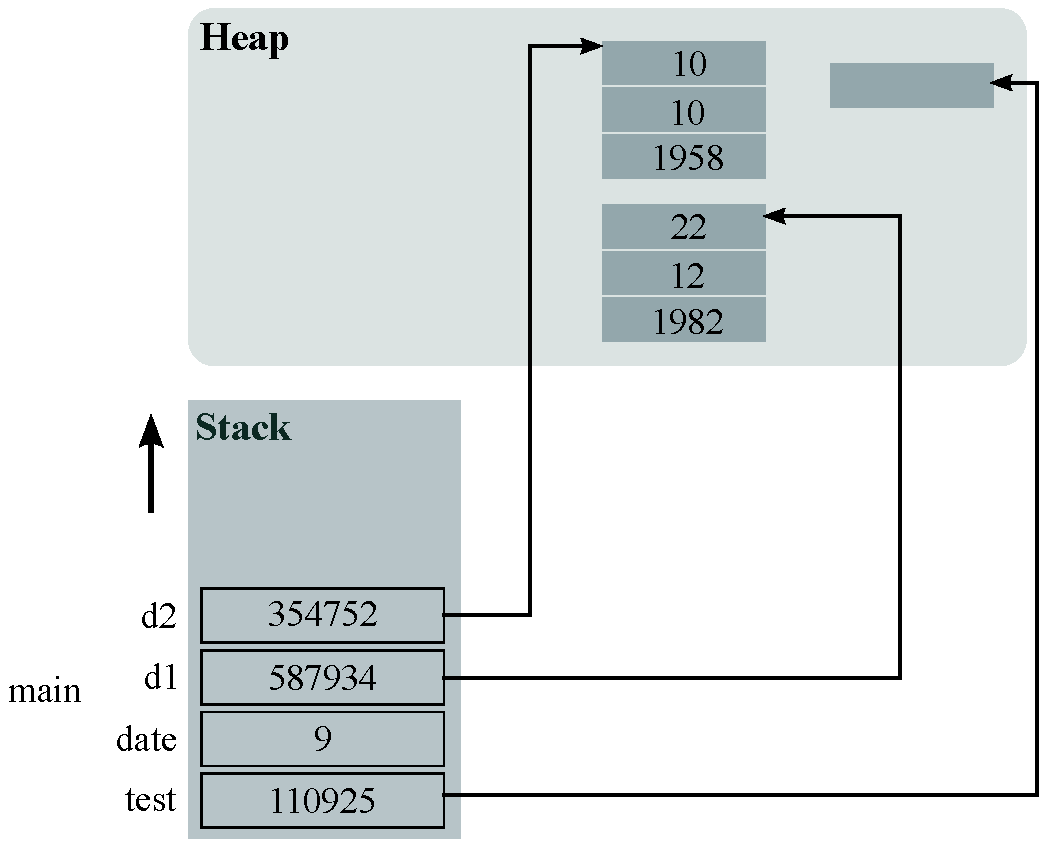
\includegraphics[width=\textwidth]{images/Java-memory-allocation/fig01.pdf}
  \end{minipage}%
  \begin{minipage}[t]{0.5\linewidth}
    \centering
    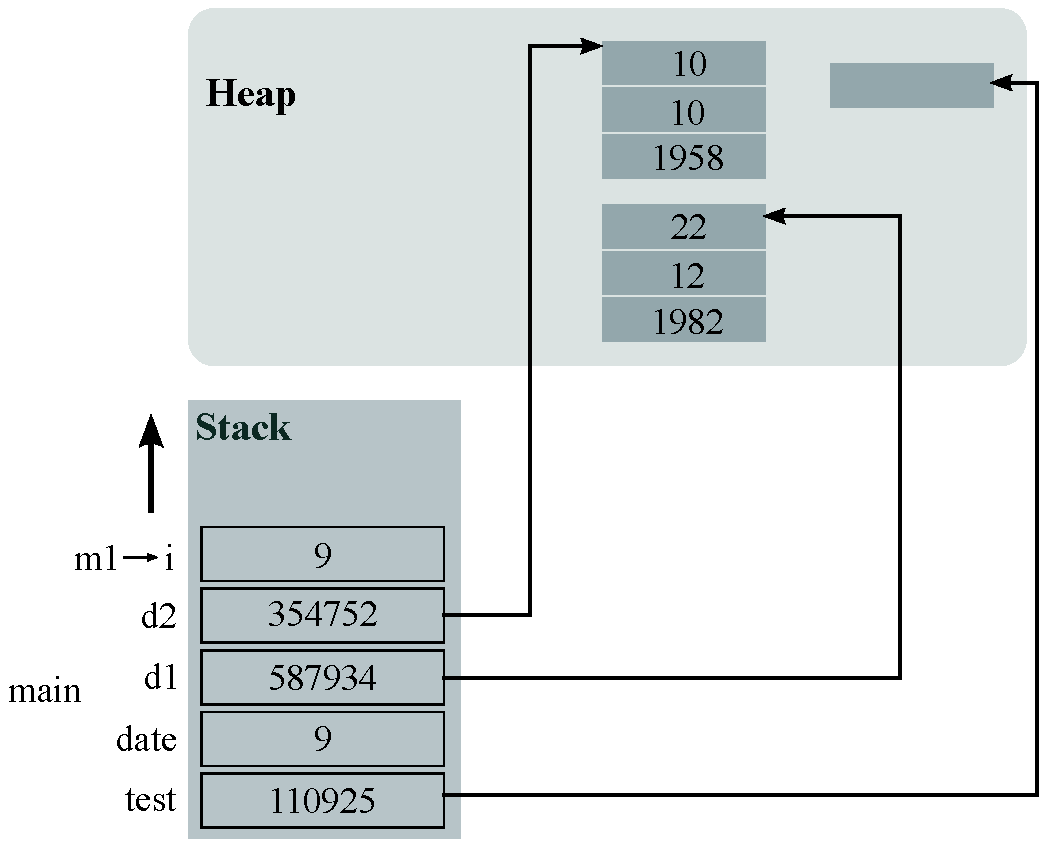
\includegraphics[width=\textwidth]{images/Java-memory-allocation/fig02.pdf}
  \end{minipage}
\end{figure}

\begin{figure}[htb]
  \begin{minipage}[t]{0.5\linewidth}
    \centering
    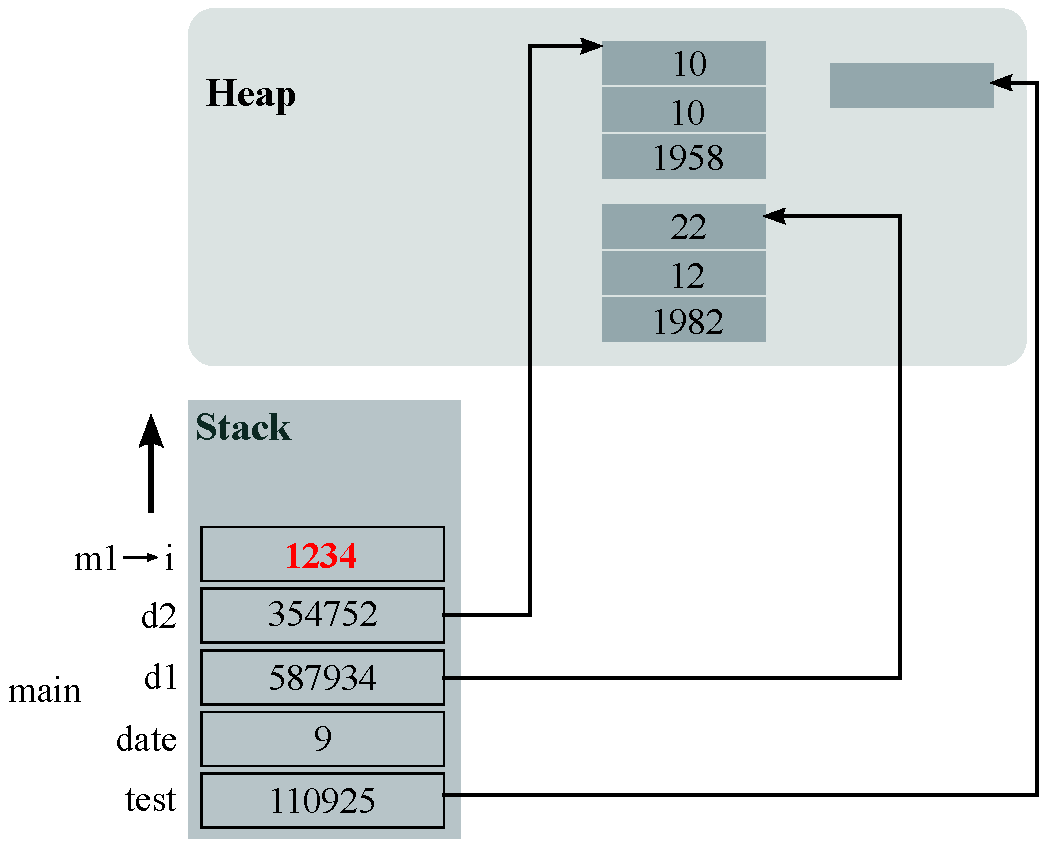
\includegraphics[width=\textwidth]{images/Java-memory-allocation/fig03.pdf}
  \end{minipage}%
  \begin{minipage}[t]{0.5\linewidth}
    \centering
    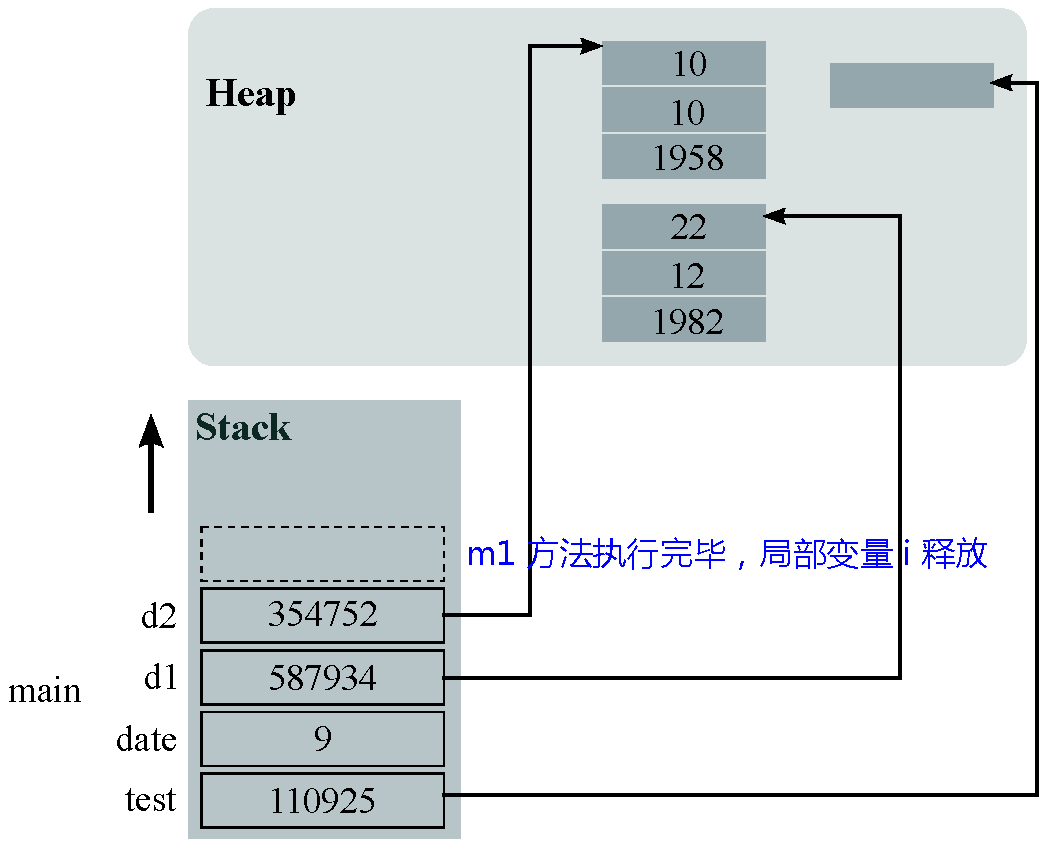
\includegraphics[width=\textwidth]{images/Java-memory-allocation/fig04.pdf}
  \end{minipage}
\end{figure}

\begin{figure}[htb]
  \begin{minipage}[t]{0.5\linewidth}
    \centering
    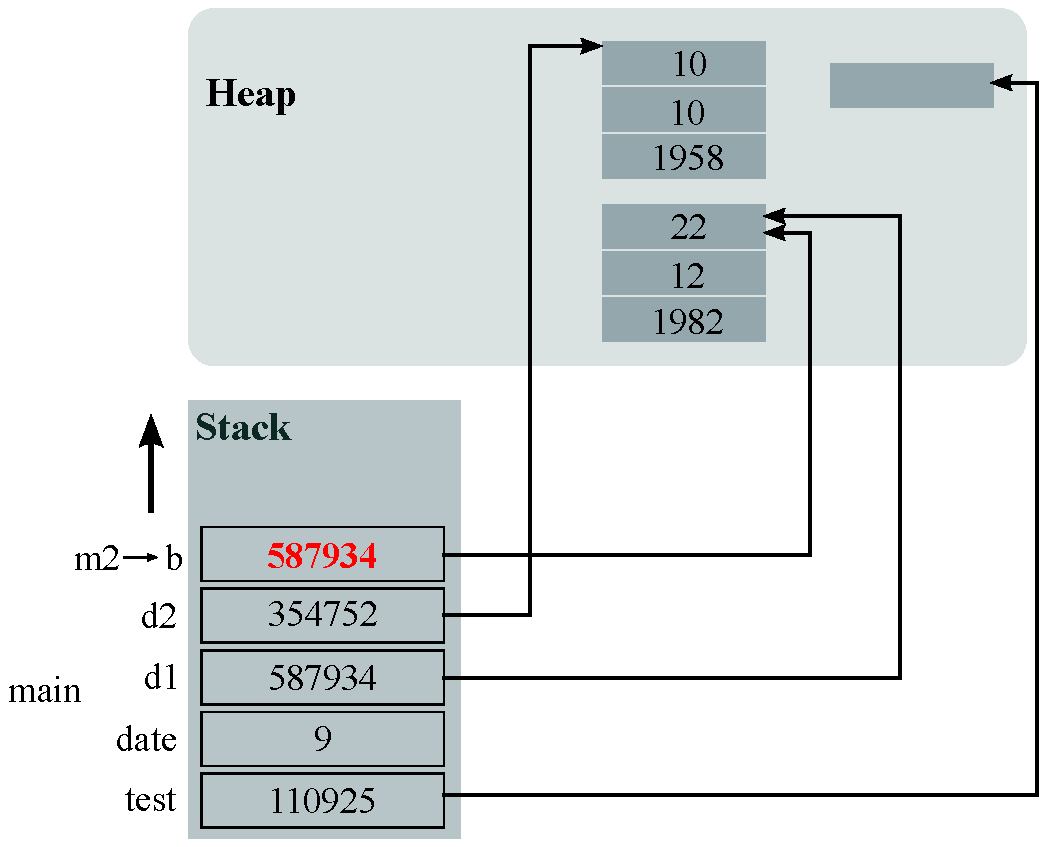
\includegraphics[width=\textwidth]{images/Java-memory-allocation/fig05.pdf}
  \end{minipage}%
  \begin{minipage}[t]{0.5\linewidth}
    \centering
    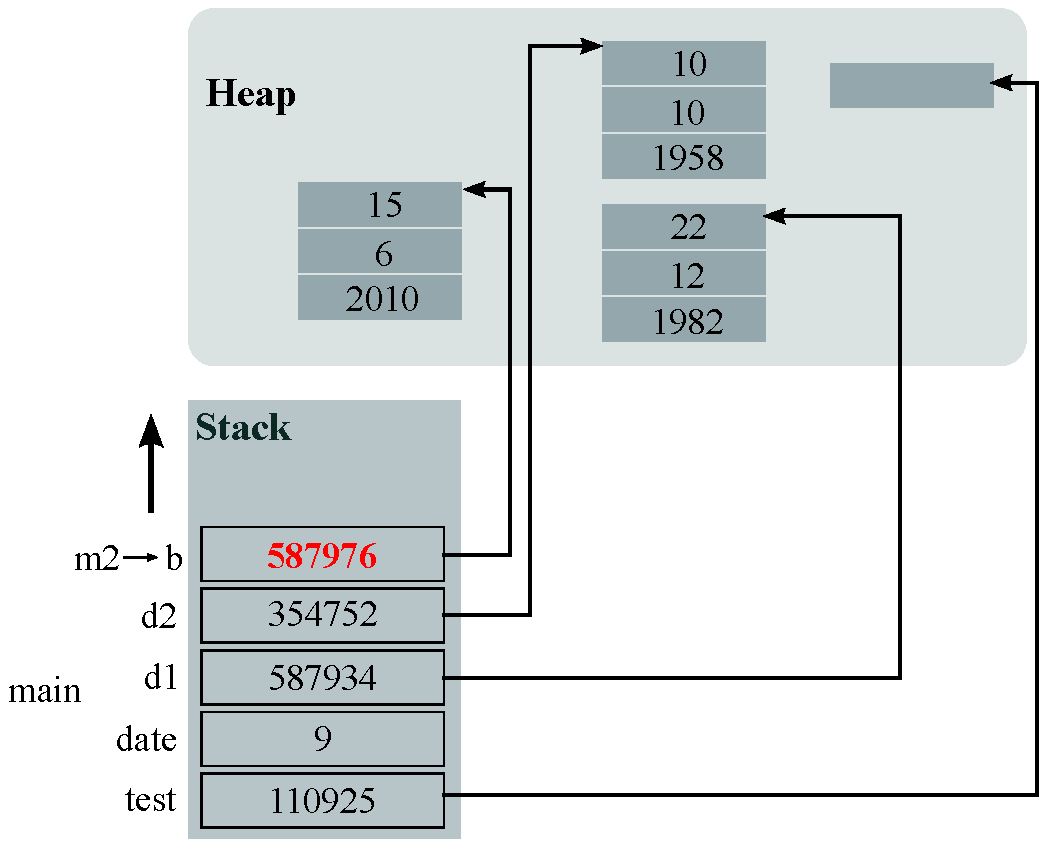
\includegraphics[width=\textwidth]{images/Java-memory-allocation/fig06.pdf}
  \end{minipage}
\end{figure}

\subsection{Java程序运行内存分析小结}

\begin{itemize}
\item 基本类型和引用类型,二者作为局部变量时都存放在栈中。
\item 基本类型直接在栈中保存值,引用类型在栈中保存一个指向堆区的指针,
  真正的对象存放在堆中。
\item 作为参数时基本类型就直接传值,引用类型传指针。
\end{itemize}

\notice{注意什么是对象}

\begin{javaCode}
  MyClass a = new MyClass();
\end{javaCode}

此时a是指向对象的指针,而不能说a是对象。指针存储在栈中,对象存储在堆中,
操作实例实际上是通过指针间接操作对象。多个指针可以指向同一个对象。

\begin{itemize}
\item {\hei\Red 栈中的数据和堆中的数据销毁并不是同步的。}方法一旦执行结
    束,栈中的局部变量立即销毁,但是堆中对象不一定销毁。因为可能有其
    他变量也指向了这个对象,直到栈中没有变量指向堆中的对象时,它才销
    毁;而且还不是马上销毁,要等垃圾回收扫描时才可以被销毁。
\item {\hei\Red 栈、堆、代码段、数据段等都是相对于应用程序而言的。}每一
    个应用程序都对应唯一的一个JVM实例,每一个JVM实例都有自己的内存区
    域,互不影响,并且这些内存区域是该JVM实例所有线程共享的。
\end{itemize}

\section{Java内存管理建议}

\subsection{Java垃圾回收机制} 

{\hei\Blue JVM的垃圾回收机制(GC)决定对象是否是垃圾对象,并进行回收。}垃圾回收机制的特点包括:

\begin{itemize}
\item 垃圾内存并不是用完了马上就被释放,所以会产生内存释放不及时的现象,
  从而降低内存的使用效率。而当程序庞大的时候,这种现象更为明显。
\item 垃圾回收工作本身需要消耗资源,同样会产生内存浪费。
\end{itemize}

JVM中的对象生命周期一般分为7个阶段:\ding{182}创建阶段、\ding{183}应用
阶段、\ding{184}不可视阶段、\ding{185}不可到达阶段、\ding{186}可收集阶
段、\ding{187}终结阶段、\ding{188}释放阶段。

Java需要内存管理,在JVM中运行的对象的整个生命周期中,进行人为的内存管理是必要的,主要原因体现在:

\begin{itemize}
\item 虽然JVM已经代替开发者完成了对内存的管理,但是硬件本身的资源是有限的。
\item 如果Java的开发人员不注意内存的使用依然会造成较高的内存消耗,导致性能的降低。
\end{itemize}

\subsection{JVM内存溢出和参数调优}

\notice{当遇到OutOfMemoryError时该如何做?}

\begin{itemize}
\item 常见的OOM(Out Of Memory)内存溢出异常,就是堆内存空间不足以存放
  新对象实例时导致。
\item 永久区内存溢出相对少见,一般是由于需要加载海量的Class数据,超过了
  非堆内存的容量导致。通常出现在Web应用刚刚启动时。因此Web应用推荐使用
  预加载机制,方便在部署时就发现并解决该问题。
 \item 栈内存也会溢出,但是更加少见。
\end{itemize}

对内存溢出的处理方法不外乎这两种:\ding{182} 调整JVM内存配置;\ding{183} 优化代码。

创建阶段的JVM内存配置优化需要关注以下项:

\begin{description}
\item[堆内存优化] 调整JVM启动参数 -Xms -Xmx -XX:newSize -XX:MaxNewSize,
  如调整初始堆内存和最大对内存 -Xms256M -Xmx512M。 或者调整初始New
  Generation的初始内存和最大内存 -XX:newSize=128M -XX:MaxNewSize=128M。
\item[永久区内存优化] 调整PermSize参数,如 -XX:PermSize=256M
  -XX:MaxPermSize=512M。
 \item[栈内存优化] 调整每个线程的栈内存容量,如 -Xss2048K。
\end{description}

\subsection{内存优化的小示例}

\subsubsection{减少无谓的对象引用创建}

\samp{Test 1}

\begin{javaCode}
  for(int i=0; i<10000; i++) {
    Object obj = new Object(); 
  }
\end{javaCode}

\samp{Test 2}

\begin{javaCode}
  Object obj = null; 
  for( int i=0; i<10000; i++) {
    obj = new Object(); 
  }
\end{javaCode}

\descript{内存性能分析}
  
{\small\kai Test 2比Test 1的性能要好。两段程序每次执行for循环都要创建一
  个Object的临时对象,JVM的垃圾回收不会马上销毁但这些临时对象。相对
  于Test 1,Test 2则只在栈内存中保存一份对象的引用,而不必创建大量新临
  时变量,从而降低了内存的使用。}


\subsubsection{不要对同一对象初始化多次}

\begin{javaCode}
  public class A { 
    private Hashtable table = new Hashtable(); 
    public A() { 
      table = new Hashtable();
    }
  }
\end{javaCode}

\descript{内存性能分析}

{\small\kai 上述代码new了两个Hashtable,但是却只使用了一个,另外一个则
  没有被引用而被忽略掉,浪费了内存。并且由于进行了两次new操作,也影响了
  代码的执行速度。另外,不要提前创建对象,尽量在需要的时候创建对象。}

\subsection{对象其他生命周期阶段内存管理}

\begin{description}
\item[应用] 即该对象至少有一个引用在维护它。
\item[不可视] 即超出该变量的作用域。\\{\kai 因为JVM GC并不是马上进行回
    收,而是要判断对象是否被其他引用维护。所以,如果我们在使用完一个对
    象以后对其进行obj = null或者obj.doSomething()操作,将其标记为空,则
    帮助JVM及时发现这个垃圾对象。}
\item[不可到达] 即在JVM中找不到对该对象的直接或者间接的引用。
\item[可收集,终结,释放] 垃圾回收器发现该对象不可到达,finalize方法已
  经被执行,或者对象空间已被重用的时候。
\end{description}

\subsubsection{Java的finalize()方法}

Java所有类都继承自Object类,而finalize()是Object类的一个函数,该函数
在Java中类似于C++的析构函数(仅仅是类似)。一般来说可以通过重
载finalize()的形式来释放类中对象。

\begin{javaCode}
  public class A { 
    public Object a; 

    public A() { 
      a = new Object() ;
    } 
    
    protected void finalize() throws java.lang.Throwable { 
      a = null; // 标记为空,释放对象 
      super.finalize(); // 递归调用超类中的 finalize 方法
    }
  } 
\end{javaCode}

什么时候finalize()被调用由JVM来决定。{\hei\Blue 尽量少用finalize()函
  数,finalize()函数是Java提供给程序员一个释放对象或资源的机会。但它会
  加大GC的工作量,因此尽量少采用finalize方式回收资源。}

\begin{itemize}
\item 一般的,纯Java编写的Class不需要重写finalize()方法,因为Object已
  经实现了一个默认的,除非我们要实现特殊的功能。
\item 用Java以外的代码编写的Class(比如JNI、C++的new方法分配的内存),
  垃圾回收器并不能对这些部分进行正确的回收,这就需要我们覆盖默认的方
  法来实现对这部分内存的正确释放和回收。
\end{itemize}

\newpage
\section*{实验设计}
\sline

%% Week 04 %%
%%%%%%%%%%%%%%%%%%%%%%%%%%%%%%%%%%%%%%%%%%%%%%%%%%%%%%%%%%%%%%%%%%%%%%%%%%%%%%%
% Full instructions available at:
% https://github.com/elauksap/focus-beamertheme

\documentclass{beamer}
\usetheme{focus}

% package for font
\usepackage{fontspec}
\defaultfontfeatures{Mapping=tex-text}  %%如果没有它,会有一些 tex 特殊字符无法正常使用,比如连字符。
\usepackage{xunicode,xltxtra}
\usepackage[BoldFont,SlantFont,CJKnumber,CJKchecksingle]{xeCJK}  % \CJKnumber{12345}: 一万二千三百四十五
\usepackage{CJKfntef}  %%实现对汉字加点、下划线等。
\usepackage{pifont}  % \ding{}
% package for math
\usepackage{amsfonts}
% package for graphics
\usepackage[americaninductors,europeanresistors]{circuitikz}
\usepackage{tikz}
\usetikzlibrary{plotmarks}  % placements=positioning
\usepackage{graphicx}  % \includegraphics[]{}
\usepackage{subfigure}  %%图形或表格并排排列
% package for table
\usepackage{colortbl,dcolumn}  %% 彩色表格
\usepackage{multirow}
\usepackage{multicol}
\usepackage{booktabs}
% package for code
\usepackage{fancyvrb}
\usepackage{listings}
% setting for font
%%\setCJKmainfont{Adobe Kaiti Std}
\setCJKmainfont{SimSun}
%%\setCJKmainfont{Microsoft YaHei}
%%\setCJKmainfont{FangSong_GB2312} 
%%\setmainfont{Times New Roman}
%\setsansfont[Mapping=tex-text]{Adobe Song Std}
%如果装了Adobe Acrobat,可在font.conf中配置Adobe字体的路径以使用其中文字体。
%也可直接使用系统中的中文字体如SimSun、SimHei、微软雅黑等。
%原来beamer用的字体是sans family;注意Mapping的大小写,不能写错。
%设置字体时也可以直接用字体名,以下三种方式等同:
%\setromanfont[BoldFont={黑体}]{宋体}
%\setromanfont[BoldFont={SimHei}]{SimSun}
%\setromanfont[BoldFont={"[simhei.ttf]"}]{"[simsun.ttc]"}

% font setting by xeCJK
\setCJKfamilyfont{NSimSun}{NSimSun}
\newcommand{\song}{\CJKfamily{NSimSun}}
%%%\setCJKfamilyfont{AdobeSongStd}{Adobe Song Std}
%%%\newcommand{\AdobeSong}{\CJKfamily{AdobeSongStd}}
\setCJKfamilyfont{FangSong}{FangSong_GB2312}
\newcommand{\fang}{\CJKfamily{FangSong}}
%%%\setCJKfamilyfont{AdobeFangsongStd}{Adobe Fangsong Std}
%%%\newcommand{\AdobeFang}{\CJKfamily{AdobeFangsongStd}}
\setCJKfamilyfont{SimHei}{SimHei}
\newcommand{\hei}{\CJKfamily{SimHei}}
%%%\setCJKfamilyfont{AdobeHeitiStd}{Adobe Heiti Std}
%%%\newcommand{\AdobeHei}{\CJKfamily{AdobeHeitiStd}}
\setCJKfamilyfont{KaiTi}{KaiTi_GB2312}
\newcommand{\kai}{\CJKfamily{KaiTi}}
%%%\setCJKfamilyfont{AdobeKaitiStd}{Adobe Kaiti Std}
\newcommand{\AdobeKai}{\CJKfamily{AdobeKaitiStd}}
\setCJKfamilyfont{LiSu}{LiSu}
\newcommand{\li}{\CJKfamily{LiSu}}
\setCJKfamilyfont{YouYuan}{YouYuan}
\newcommand{\you}{\CJKfamily{YouYuan}}
\setCJKfamilyfont{FZJingLei}{FZJingLeiS-R-GB}
\newcommand{\jinglei}{\CJKfamily{FZJingLei}}
\setCJKfamilyfont{MSYH}{Microsoft YaHei}
\newcommand{\msyh}{\CJKfamily{MSYH}}

\setbeamerfont{frametitle}{series=\Large\hei} % 修改Beamer标题字体

\graphicspath{{figures/}}  %%图片路径
\renewcommand\figurename{图}

% setting for pdf
\hypersetup{% pdfpagemode=FullScreen,%
  pdfauthor={Xiaodong Wang},%
  pdftitle={Title},%
  CJKbookmarks=true,%
  bookmarksnumbered=true,%
  bookmarksopen=false,%
  plainpages=false,%
  colorlinks=true,%
  citecolor=green,%
  filecolor=magenta,%
  linkcolor=blue,%red(default)
  urlcolor=cyan}

% setting for fontspec
\XeTeXlinebreaklocale "zh"  %%表示用中文的断行
\XeTeXlinebreakskip = 0pt plus 1pt minus 0.1pt  %%多一点调整的空间
%%%%%

% 自定义颜色
\def\Red{\color{red}}
\def\Green{\color{green}}
\def\Blue{\color{blue}}
\def\Mage{\color{magenta}}
\def\Cyan{\color{cyan}}
\def\Brown{\color{brown}}
\def\White{\color{white}}
\def\Black{\color{black}}

\lstnewenvironment{xmlCode}[1][]{% for Java
  \lstset{
    basicstyle=\tiny\ttfamily,%
    columns=flexible,%
    framexleftmargin=.7mm, %
    % frame=shadowbox,%
    % rulesepcolor=\color{cyan},%
     frame=single,%
    backgroundcolor=\color{white},%
    xleftmargin=4\fboxsep,%
    xrightmargin=4\fboxsep,%
    numbers=left,numberstyle=\tiny,%
    numberblanklines=false,numbersep=7pt,%
    language=xml, %
    }\lstset{#1}}{}

\lstnewenvironment{javaCode}[1][]{% for Java
  \lstset{
    basicstyle=\tiny\ttfamily,%
    columns=flexible,%
    framexleftmargin=.7mm, %
    frame=shadowbox,%
    rulesepcolor=\color{cyan},%
    % frame=single,%
    backgroundcolor=\color{white},%
    xleftmargin=4\fboxsep,%
    xrightmargin=4\fboxsep,%
    numbers=left,numberstyle=\tiny,%
    numberblanklines=false,numbersep=7pt,%
    language=Java, %
    }\lstset{#1}}{}

\lstnewenvironment{shCode}[1][]{% for Java
  \lstset{
    basicstyle=\scriptsize\ttfamily,%
    columns=flexible,%
    framexleftmargin=.7mm, %
    frame=shadowbox,%
    rulesepcolor=\color{brown},%
    % frame=single,%
    backgroundcolor=\color{white},%
    xleftmargin=4\fboxsep,%
    xrightmargin=4\fboxsep,%
    numbers=left,numberstyle=\tiny,%
    numberblanklines=false,numbersep=7pt,%
    language=sh, %
    }\lstset{#1}}{}

\newcommand\ask[1]{\vskip 4bp \tikz \node[rectangle,rounded corners,minimum size=6mm,
  fill=white,]{\Cyan \includegraphics[height=1.5cm]{question} \Large \msyh #1};}

\newcommand\wxd[1]{\vskip 4bp \tikz \node[rectangle,minimum size=6mm,
  fill=blue!60!white,]{\White \ding{118} \msyh #1};}

\newcommand\cxf[1]{\vskip 4bp \tikz \node[rectangle,rounded corners,minimum size=6mm,
  fill=purple!60!white,]{\White \ding{42} \msyh #1};}

\newcommand\xyy[1]{\vskip 2bp \tikz \node[rectangle,minimum size=3mm,
  fill=black!80!white,]{\White \msyh\scriptsize #1};}

\newcommand\tta[1]{\vskip 4bp \tikz \node[rectangle,minimum size=6mm,
  fill=blue!60!white,]{\White \ding{118} \msyh #1};}

\newcommand\ttb[1]{\vskip 4bp \tikz \node[rectangle,rounded corners,minimum size=6mm,
  fill=purple!60!white,]{\White \ding{42} \msyh #1};}

\newcommand\ttc[1]{\vskip 2bp \tikz \node[rectangle,minimum size=3mm,
  fill=black!80!white,]{\White \msyh\scriptsize #1};}

\newcommand\homework[1]{\vskip 2bp \tikz \node[rectangle,minimum size=3mm,
  fill=red!80!white,]{\White \ding{45} \msyh\scriptsize 课后小作业 } ; {\kai\small #1}} 

\newcommand\notice[1]{\vskip 4bp \tikz \node[rectangle,rounded corners,minimum size=6mm,
  fill=red!80!white,]{\White \scriptsize \ding{42} \msyh #1};}

\newcommand\samp[1]{\vskip 2bp \tikz \node[rectangle,minimum size=3mm,]{\Mage\msyh \small CODE \ding{231} \Black #1};\vskip -8bp}

\newcommand\codeset[1]{\vskip 2bp \tikz \node[rectangle,minimum
  size=3mm]{\Mage\msyh \small 课程配套代码 \ding{231} \Black
    #1};\vskip -4bp}

\newcommand\pptlink[2]{\vskip 4bp \tikz \node[rectangle,rounded corners,minimum size=6mm,
  fill=blue!70!white,]{\href{run:#1}{\White \scriptsize \msyh 动画演示 #2}};}


\makeatletter
\newcommand{\Extend}[5]{\ext@arrow 0099{\arrowfill@#1#2#3}{#4}{#5}}
\makeatother
%%%%%%%%%%%%%%%%%%%%%%%%%%%%%%%%%%%%%%%%%%%%%%%%%%%%%%%%%%%%%%%%%%%%%%%%%%%%%%%
\title{\hei JAVA应用与开发\\  高级类特性}
\subtitle{\it 让我们愉快的Coding起来吧...}
\author{王晓东}
\titlegraphic{\vspace{-8em}
\includegraphics[height=10cm]{static/ouc.pdf}\vspace{-6em}} 
\institute{中国海洋大学信息学院计算机系}
\date{\today}

\begin{document}
\begin{frame}
  \maketitle
\end{frame}

\begin{frame}
  \frametitle{学习目标}
  \begin{itemize}
  \item 掌握抽象类和接口的概念、特性及定义方法
  \item 理解抽象类和接口的异同和作用
  \item 了解嵌套类的分类,掌握嵌套类中静态嵌套类和匿名嵌套类的概念
  \item 掌握匿名内部类的特征、继承和接口实现的用法
  \item 掌握枚举类型的使用方法
  \end{itemize}
\end{frame}

\begin{frame}
  \frametitle{大纲}
  \tableofcontents
\end{frame}

\section{抽象类}

\begin{frame}[fragile]
  \frametitle{什么是抽象类}

  \begin{columns}
    \column{0.7\textwidth}
    \begin{alertblock}{抽象类}
      在面向对象的概念中,所有的对象都是通过类来描绘的,但是反过来,并不
      是所有的类都是用来描绘对象的。如果一个类中没有包含足够的信息来描绘
      一个具体的对象,这样的类就是抽象类。
    \end{alertblock}
    \pause
    \begin{block}{}
      抽象类往往用来表征对问题领域进行分析、设计中得出的抽象概念,是对一
      系列看上去不同但是本质上相同的具体概念的抽象。
    \end{block}

    \column{0.3\textwidth}
    \begin{figure}
      \centering
      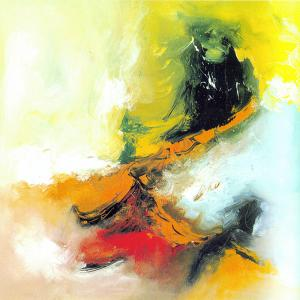
\includegraphics[width=\textwidth]{fig-i-am-abstract.jpg}
      \caption{我很抽象}
      \label{fig:i-am-abstract}
    \end{figure}
  \end{columns}
\end{frame}

\begin{frame}[fragile] % [fragile]参数使得能够插入代码
  \frametitle{定义抽象类}

  \begin{block}{}
    \begin{itemize}
    \item 在定义Java方法时可以只给出方法头,而不必给出方法的实现细节,这
      样的方法被称为{\Red 抽象方法}。
    \item 抽象方法必须用关键字{\Red abstract}修饰。
    \item 包含抽象方法的类必须声明为抽象类,用关键字{\Red abstract}修
      饰。
    \end{itemize}
  \end{block}


  \samp{抽象类示例}
  
  \begin{javaCode}
    public abstract class Animal { //定义为抽象类
      private int age;
      
      public void setAge(int age) {
        this.age = age;
      }
      
      public int getAge(){
        return age;
      }
      
      public abstract void eat(); //抽象方法
    }
  \end{javaCode}
\end{frame}

\begin{frame}[fragile] % [fragile]参数使得能够插入代码
  \frametitle{定义抽象类}

  \samp{抽象类继承}
  
  \begin{javaCode}
    public class Person extends Animal {
      private String name;
      public void setName(String name) {
        this.name = name;
      }
      public String getName() {
        return name;
      }
      public void eat() { //重写方法
        System.out.println("洗手→烹饪→摆餐具→吃喝→收摊儿");
      }
    }
  \end{javaCode}

  \begin{javaCode}
    public class Bird extends Animal {
      public void fly(){
        System.out.println("我心飞翔!");
      }
      public void eat(){  //重写方法
        System.out.println("直接吞食!");
      }
    }
  \end{javaCode}
\end{frame}

\begin{frame}[fragile] % [fragile]参数使得能够插入代码
  \frametitle{抽象类的特性与作用}

  \tta{抽象类的特性}

  \begin{itemize}[<+-| alert@+>]
  \item 子类必须实现其父类中的所有抽象方法,否则该子类也只能声明为抽象类。
  \item 抽象类不能被实例化。\pause\notice{问题} 抽象类能否有构造方法?
  \end{itemize}
  
  \pause
  
  \tta{抽象类的作用}
  
  抽象类主要是通过继承由其子类发挥作用,包括两方面:
  
  \begin{description}
  \item[\fbox{代码重用}] 子类可以重用抽象类中的属性和非抽象方法。
  \item[\fbox{规划}] 子类中通过抽象方法的重写来实现父类规划的功能。
  \end{description}
\end{frame}


\begin{frame}[fragile] % [fragile]参数使得能够插入代码
  \frametitle{抽象类的其他特性}
  
  \begin{itemize}[<+-| alert@+>]
  \item 抽象类中可以不包含抽象方法。{\kai 主要用于当一个类已经定义了多
      个更适用的子类时,为避免误用功能相对较弱的父类对象,干脆限制其实
      例化。}
  \item 子类中可以不全部实现抽象父类中的抽象方法,但此时子类也只能声明为抽象类。
  \item 父类不是抽象类,但在子类中可以添加抽象方法,此情况下子类必须声明为抽象类。
  \item 多态性对于抽象类仍然适用,可以将引用类型变量(或方法的形参)声明为抽象类的类型。
  \item 抽象类中可以声明static属性和方法,只要访问控制权限允许,这些属性和方法可以通
    过{\kai <类名>.<类成员>}的方法进行访问。
  \end{itemize}
\end{frame}

\section{接口}

\begin{frame}[fragile] % [fragile]参数使得能够插入代码
  \frametitle{接口(interface)}

  \begin{block}{接口}
    在科技辞典中,“接口”被解释为“两个不同系统(或子程序)交接并通过它
    彼此作用的部分。”
  \end{block}

  \pause

  在Java语言中,通过接口可以了解对象的交互界面,即明确对象提供的功能及
  其调用格式,而不需要了解其实现细节。

  \pause

  接口是抽象方法和常量值的定义的集合。从本质上讲,接口是一种特殊的{\Red 抽象
  类},这种抽象类中{\kai\Red 只包含常量定义和方法声明,而没有变量和方法的实现}。
\end{frame}

\begin{frame}[fragile] % [fragile]参数使得能够插入代码
\frametitle{定义接口}

接口中定义的属性必须是public static final的,而接口中定义的方法则必须
是public abstract的,因此这些关键字可以部分或全部省略。

\samp{接口示例(未简化)}

\begin{javaCode}
  public interface Runner {
    public static final int id = 1;
    public abstract void start();
    public abstract void run();
    public abstract void stop();
  }
\end{javaCode}

\samp{与上述代码等价的标准定义}

\begin{javaCode}
  public interface Runner {
    int id = 1;
    void start();
    void run();
    void stop();
  }
\end{javaCode}
\end{frame}

\begin{frame}[fragile] % [fragile]参数使得能够插入代码
  \frametitle{接口的实现}

  和继承关系类似,类可以{\Red\hei 实现}接口,且接口和实现类之间也存在多态性。

  \tta{类继承和接口实现的语法格式}

  \begin{javaCode}
    [<modifier>] class <name> [extends <superclass>] [implements <interface> [,<interface>]* ] {
      <declarations>*
    }
  \end{javaCode}
\end{frame}

\begin{frame}[fragile] % [fragile]参数使得能够插入代码
  \frametitle{接口的实现}

  \samp{接口实现示例}

  \begin{javaCode}
    public class Person implements Runner {
      public void start() {
        System.out.println("弯腰、蹬腿、咬牙、瞪眼、开跑");
      }
      public void run(){
        System.out.println("摆动手臂、维持直线方向");
      }
      public void stop(){
        System.out.println("减速直至停止、喝水");
      }
    }
  \end{javaCode}
\end{frame}

\begin{frame}[fragile] % [fragile]参数使得能够插入代码
  \frametitle{接口的实现}

  通过接口可以指明多个类需要实现的方法,而这些类还可以根据需要继承各自
  的父类。或者说,{\Red\kai 通过接口可以实现不相关类的相同行为,而不需要考
    虑这些类之间的层次关系。}
  
  \begin{figure}
    \centering
    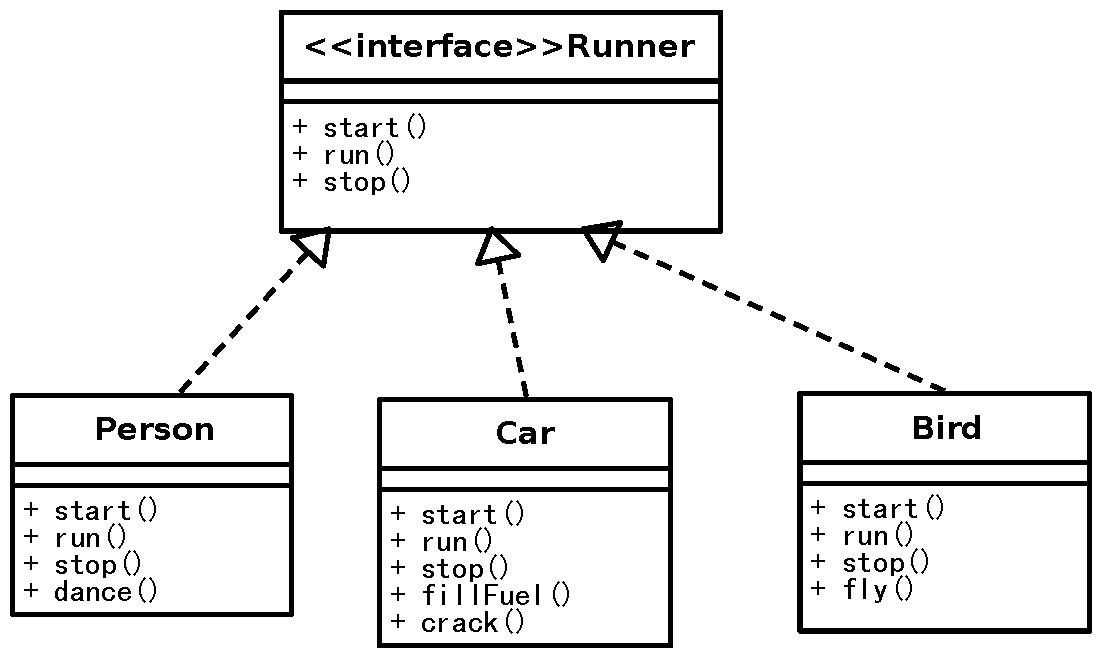
\includegraphics[width=0.5\textwidth]{fig-interface-implement-sample.pdf}
  \end{figure}

  \notice{类允许实现多重接口}

  \codeset{package sample.advance.interfacesample}

\end{frame}


\begin{frame}[fragile] % [fragile]参数使得能够插入代码
\frametitle{接口间的继承}

与接口的多重实现情况类似,由于不担心方法追溯调用上的不确定性,接口之间
的继承允许“多重继承”的情况。

\begin{javaCode}
interface A {
  public void ma();
}
interface B {
  public int mb(int i);
}
interface C extends A,B {  //接口的多重继承
  public String mc();
}
class D implements C {
  public void ma() {
    System.out.println("Implements method ma()!");
  }
  public int mb(int i) {
    return 2000 + i;
  }
  public String mc() {
    return "Hello!";
  }
}
\end{javaCode}
{\footnotesize \Mage 上述代码中的D类缺省继承了Object类,直接实现了接口C,间接实现了接口A和B,由于多态性的机
制,将来D类的对象可以当作Object、C、A或B等类型使用。}
\end{frame}

\begin{frame}[fragile] % [fragile]参数使得能够插入代码
  \frametitle{接口特性总结}

  \begin{itemize}[<+-| alert@+>]
  \item 通过接口可以实现不相关类的相同行为,而不需要考虑这些类之间的层次关系。
  \item 接口可以被多重实现。
  \item 接口可以继承其它的接口,并添加新的属性和抽象方法,接口间支持多重继承。
  \end{itemize}
\end{frame}
%%%%%%%%%%%%%%%%%%%%%%%%%%%%%%%%%%%%%%%%%%%%%%%%
\section{抽象类和接口剖析}

\begin{frame}[fragile]
  \frametitle{语法层面的区别}

  \begin{alertblock}{}
    \hei\centering 概念差异 —— 语法差异 —— 用法差异 —— 设计哲学
  \end{alertblock}

  \pause
  
  \begin{itemize}[<+-| alert@+>]
  \item 抽象类可以提供成员方法的实现细节,而接口中只能存在public
    abstract方法
  \item 抽象类中的成员变量可以为各种类型,而接口中的成员变量只能
    是public static final类型
  \item 抽象类可以有静态代码块和静态方法,接口中不能含有静态代码块以及
    静态方法
  \item 一个类只能继承一个抽象类,而一个类却可以实现多个接口
  \end{itemize}
\end{frame}

\begin{frame}[fragile]
  \frametitle{设计层面的区别}

  \begin{block}{}
    \begin{itemize}\kai
    \item 抽象类是对类的抽象(可以抽象但不宜实例化),而接口是对行为的
      抽象。
    \item 抽象类是对类整体进行抽象,包括属性、行为,但是接口却是对类局
      部(行为)进行抽象。
    \end{itemize}
  \end{block}

  \pause

  \begin{block}{}
    \begin{itemize}\kai
    \item 抽象类作为很多子类的父类,它是一种模板式设计。{\Red 模板式设计:模
      板代表公共部分,公共部分需要改的则改动模板即可。}
    \item 而接口是一种行为规范,它是一种辐射式设计。{\Red 辐射式设计:接口
      进行了变更,则所有实现类都必须进行相应的改动。}
    \end{itemize}
  \end{block}  

\end{frame}

\begin{frame}[fragile]
  \frametitle{怎样才是合理的设计?(门和警报的示例)}

  一般来说,门都有\fbox{open()}和\fbox{close()}这两个动作。通过抽象类和
  接口来定义这个抽象概念:

  \begin{columns}
    \column{0.5\textwidth}

    \begin{javaCode}
      abstract class Door {
        public abstract void open();
        public abstract void close();
      }
    \end{javaCode}
    \column{0.5\textwidth}

    \begin{javaCode}
      interface Door {
        public abstract void open();
        public abstract void close();
      }
    \end{javaCode}
  \end{columns}

  \pause
  
  \notice{问题} 如果现在我们需要门具有报警\fbox{alarm()}的功能该如何实
  现?
\end{frame}

\begin{frame}[fragile]
  \frametitle{怎样才是合理的设计?(门和警报的示例)}

  \tta{思路一} 
  
  将这三个功能都放在抽象类里面,这样一来所有继承这个抽象类的子类都具备
  了报警功能,但是有的门并不一定需要具备报警功能。\pause {\hei\Red 不合理抽象}

  \pause
  
  \tta{思路二} 

  将这三个功能都放在接口里面,但需要用到报警功能的类就需要实现这个接口
  中的open()和close(),也许这个类根本就不具备open()和close()这两个功能,
  比如火灾报警器。\pause {\hei\Red 不合理规划}

\end{frame}

\begin{frame}[fragile]
  \frametitle{怎样才是合理的设计?(门和警报的示例)}

  Door的open() 、close()和alarm()根本就属于两个不同范畴内的行为:

  \begin{itemize}
  \item open()和close()属于门本身固有的行为特性。
  \item alarm()属于延伸的附加行为。
  \end{itemize}

  \pause
  
  \tta{更为合理的思路} 

  \ding{182} 单独将报警设计为一个接口,包含alarm()行为;\ding{183} Door设计为单独
  的抽象类,包含open()和close()两种行为;\ding{184} 设计一个报警门继
  承Door类和实现Alarm接口。

  \codeset{package sample.advance.door}
\end{frame}



%% 1)抽象类是对一种事物的抽象,即对类抽象,而接口是对行为的抽象。抽象类是对整个类整体进行抽象,包括属性、行为,但是接口却是对类局部(行为)进行抽象。举个简单的例子,飞机和鸟是不同类的事物,但是它们都有一个共性,就是都会飞。那么在设计的时候,可以将飞机设计为一个类Airplane,将鸟设计为一个类Bird,但是不能将 飞行 这个特性也设计为类,因此它只是一个行为特性,并不是对一类事物的抽象描述。此时可以将 飞行 设计为一个接口Fly,包含方法fly(),然后Airplane和Bird分别根据自己的需要实现Fly这个接口。然后至于有不同种类的飞机,比如战斗机、民用飞机等直接继承Airplane即可,对于鸟也是类似的,不同种类的鸟直接继承Bird类即可。从这里可以看出,继承是一个 "是不是"的关系,而 接口 实现则是 "有没有"的关系。如果一个类继承了某个抽象类,则子类必定是抽象类的种类,而接口实现则是有没有、具备不具备的关系,比如鸟是否能飞(或者是否具备飞行这个特点),能飞行则可以实现这个接口,不能飞行就不实现这个接口。
%%
%% 2)设计层面不同,抽象类作为很多子类的父类,它是一种模板式设计。而接口是一种行为规范,它是一种辐射式设计。什么是模板式设计?最简单例子,大家都用过ppt里面的模板,如果用模板A设计了ppt B和ppt C,ppt B和ppt C公共的部分就是模板A了,如果它们的公共部分需要改动,则只需要改动模板A就可以了,不需要重新对ppt B和ppt C进行改动。而辐射式设计,比如某个电梯都装了某种报警器,一旦要更新报警器,就必须全部更新。也就是说对于抽象类,如果需要添加新的方法,可以直接在抽象类中添加具体的实现,子类可以不进行变更;而对于接口则不行,如果接口进行了变更,则所有实现这个接口的类都必须进行相应的改动。
%%
%% 下面看一个网上流传最广泛的例子:门和警报的例子:门都有open( )和close( )两个动作,此时我们可以定义通过抽象类和接口来定义这个抽象概念:
%%
%%
%%abstract class Door {
%%    public abstract void open();
%%    public abstract void close();
%%}
%%  或者:
%%
%%interface Door {
%%    public abstract void open();
%%    public abstract void close();
%%}
%%  但是现在如果我们需要门具有报警alarm( )的功能,那么该如何实现?下面提供两种思路:
%%


%%%%%%%%%%%%%%%%%%%%%%%%%%%%%%%%%%%%%%%%%%%%%%%%
\section{嵌套类}
\begin{frame}[fragile] % [fragile]参数使得能够插入代码
  \frametitle{什么是嵌套类}

  Java语言支持类的嵌套定义,即允许将一个类定义在其他类的内部,其中内层的类被称为嵌套类。

  \tta{嵌套类的分类}
  
  \begin{description}
  \item[\fbox{静态嵌套类(Static Nested Class)}] 使用static修饰的嵌套类
  \item[\fbox{内部类(Inner Class)}] 非static的嵌套类
    \begin{description}
    \item[普通内部类] 在类中的方法或语句块外部定义的非static类。
    \item[局部内部类] 定义在方法或语句块中的类,也称局部类。
    \item[匿名内部类] 定义在方法或语句块中,该类没有名字、只能在其所在
      之处使用一次。
    \end{description}
  \end{description}

  {\kai (仅讲授包含静态嵌套类和匿名内部类,其他自行学习)}
  
\end{frame}


\begin{frame}[fragile] % [fragile]参数使得能够插入代码
  \frametitle{静态嵌套类}

  \tta{静态嵌套类的特征}
  
  \begin{itemize}
  \item {\hei 静态嵌套类不再依赖/引用外层类的特定对象,只是隐藏在另一个
      类中而已。}
  \item 由于静态嵌套类的对象不依赖外层类的对象而独立存在,因而可以直接
    创建,进而也就无法在静态嵌套类中直接使用其外层类的非static成员。
  \end{itemize}

  \codeset{sample.advance.nestedclass.StaticNestedClassSample.java}
\end{frame}

%%\begin{frame}[fragile] % [fragile]参数使得能够插入代码
%%\frametitle{使用内部类\ding{182}}
%%
%%\samp{JavaSE\_03/TestInnerClass.java}
%%
%%\samp{TestInner.java}
%%\begin{javaCode}
%%class A {
%%  private int s;
%%  public class B {
%%    public void mb() {
%%      s = 100;
%%      System.out.println("在内部类 B 中 s=" + s);
%%    }
%%  }
%%  public void ma() {
%%    B i = new B();
%%    i.mb();
%%  }
%%}
%%
%%public class TestInner {
%%  public static void main(String args[]) {
%%    A o = new A();
%%    o.ma();
%%  }
%%}
%%\end{javaCode}
%%
%%{\small \Mage 上述程序编译后生成三个文件:TestInner.class, A.class, A\$B.class。}
%%\end{frame}
%%
%%\begin{frame}[fragile] % [fragile]参数使得能够插入代码
%%\frametitle{使用内部类\ding{182}}
%%
%%\wxd{TestInner.java运行时的内存状态}
%%
%%系统创建一个外层类的对象o,并将其实例变量s缺省初始化为0。
%%
%%\begin{figure}
%%\centering
%%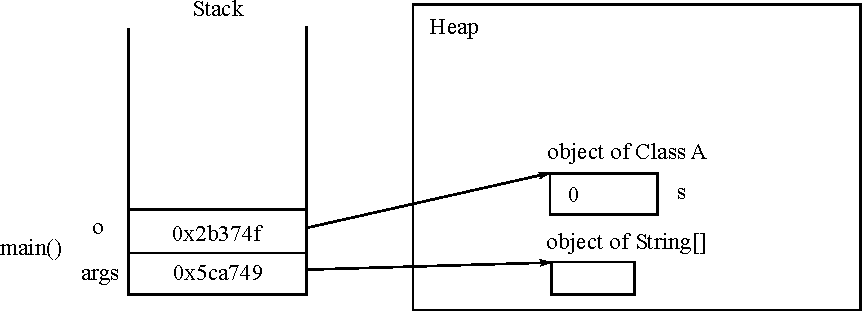
\includegraphics[width=0.8\textwidth]{innerclass01.pdf}
%%\end{figure}
%%
%%\end{frame}
%%
%%\begin{frame}[fragile] % [fragile]参数使得能够插入代码
%%\frametitle{使用内部类\ding{182}}
%%
%%\wxd{TestInner.java运行时的内存状态}
%%
%%调用对象o的成员方法ma(),首先为引用变量this分配空间以记录该方法本次运行时的当前对象,然后执行方法体中的第一条语句创建一个内部类B的对象i。
%%
%%\begin{figure}
%%\centering
%%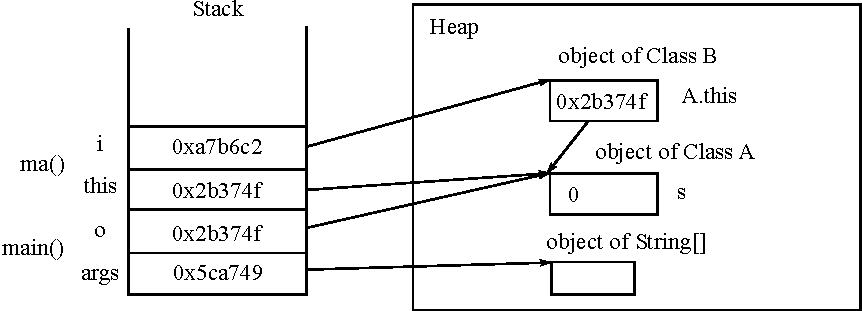
\includegraphics[width=0.8\textwidth]{innerclass02.pdf}
%%\end{figure}
%%
%%{\kai\small 此时,内部类B中虽然未显式的定义任何属性,但其对象i一经创建,即拥有一个系统自动添加的属性(实例变量),该属性的数据类型为外层类对象的句柄,该属性为只读,且可以使用约定标记<外层类名>.this访问。}
%%
%%\end{frame}
%%
%%\begin{frame}[fragile] % [fragile]参数使得能够插入代码
%%\frametitle{使用内部类\ding{182}}
%%
%%\wxd{TestInner.java运行时的内存状态}
%%
%%内部类对象i调用其成员方法mb()。
%%
%%\begin{figure}
%%\centering
%%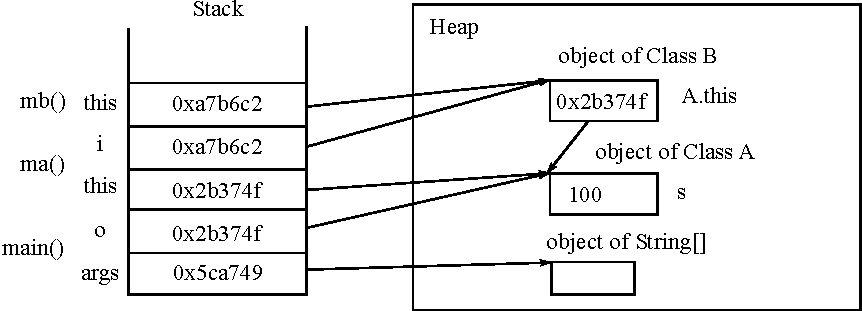
\includegraphics[width=0.8\textwidth]{innerclass03.pdf}
%%\end{figure}
%%
%%{\kai\small 在方法体中遇到变量s时,按照如下处理过程:首先在当前方法mb()中检索是否存在局部变量(包括方法形参)s,没有则继续查找方法的当前对象(内部类B中)是否存在成员变量s,没有则通过属性A.this检索当前对象所依赖的外层类对象,最终找到并操作该变量s并赋值为100。}
%%\end{frame}
%%
%%\begin{frame}[fragile] % [fragile]参数使得能够插入代码
%%\frametitle{使用内部类\ding{183}}
%%
%%在外部使用其他类中的内部类虽然不提倡,但也是允许的。此时,应指明其完整层次,并显式建立对
%%象间的依赖关系。
%%
%%\samp{A.java}
%%\begin{javaCode}
%%public class A {
%%  private int s;
%%  public class B {
%%    public void mb() {
%%      System.out.println(s);
%%    }
%%  }
%%}
%%\end{javaCode}
%%\samp{TestInner2.java}
%%\begin{javaCode}
%%public class TestInner2 {
%%  public static void main(String[] args) {
%%    A a = new A();
%%    // 创建一个依赖于 a 而存在的 b
%%    A.B b = a.new B();
%%    b.mb();
%%  }
%%}
%%\end{javaCode}
%%\end{frame}
%%
%%\begin{frame}[fragile] % [fragile]参数使得能够插入代码
%%\frametitle{使用内部类\ding{184}}
%%
%%内部类中出现变量命名冲突时,可以使用内部类对象的特殊属性“<外层类名>.this”来访问其所依赖
%%外层类对象的成员。
%%\samp{TestInner3.class}
%%\begin{javaCode}
%%class A {
%%  private int s = 111;
%%  public class B {
%%    private int s = 222;
%%    public void mb(int s) {
%%      System.out.println(s);  // 局部变量 s
%%      System.out.println(this.s);  // 内部类对象的属性 s
%%      System.out.println(A.this.s); // 外层类对象属性 s
%%    }
%%  }
%%}
%%
%%public class TestInner3 {
%%  public static void main(String args[]) {
%%    A a = new A();
%%    A.B b = a.new B();
%%    b.mb(333);
%%  }
%%}
%%\end{javaCode}
%%{\small\Mage 输出结果为:333\textbackslash n 222\textbackslash n 111}
%%\end{frame}
%%
%%\begin{frame}[fragile] % [fragile]参数使得能够插入代码
%%\frametitle{局部内部类}
%%
%%局部内部类是定义在Java方法或语句块中的类型,相当于方法中的局部变量,其作用域仅限于其所在的方法体或者语句块。
%%
%%\begin{itemize}\kai
%%\item 局部类声明时不允许加public、private等访问控制修饰符。
%%\item 局部类也不允许定义static属性和方法,{\Red 除非局部类为静态类(后续讲述)}。
%%\item 局部类中不但可以访问其所在外层类的成员,还可以访问其所在方法/语句块中的局部变量,但
%%  这些变量必须声明为{\Red final}。
%%\end{itemize}
%%
%%\samp{JavaSE\_03/TestLocalInnerClass.java}
%%
%%{\hei\Red 不建议使用局部类。}
%%\end{frame}

\begin{frame}[fragile] % [fragile]参数使得能够插入代码
\frametitle{匿名内部类}

匿名内部类是局部类的一种简化。

{\kai 当我们只在一处使用到某个类型时,可以将之定义为局部类,进而如果我
  们只是创建并使用该类的一个实例的话,那么连类的名字都可以省略。}
\end{frame}

\begin{frame}[fragile] % [fragile]参数使得能够插入代码
  \frametitle{使用匿名内部类}

  \samp{Person.java}

  \begin{javaCode}
    public abstract class Person {
      private String name;
      private int age;
      
      public Person() {}
      
      public Person(String name, int age) {
        this.name = name;
        this.age = age;
      }
      
      public String getInfo() {
        return "Name: " + name + "\t Age: " + age;
      }
      
      public abstract void work();
    }  
  \end{javaCode}
\end{frame}

\begin{frame}[fragile] % [fragile]参数使得能够插入代码
  \frametitle{使用匿名内部类}

  \samp{TestAnonymous.java}

  \begin{javaCode}
    public class TestAnonymous {
      public static void main(String[] args) {
        Person sp = new Person() { // 匿名内部类
          public void work() {
            System.out.println("个人信息:" + this.getInfo());
            System.out.println("I am sailing.");
          }
        };
        
        sp.work();
      }
    }
  \end{javaCode}

  \pause
  
  \ttc{上述代码的解释}

  {\small\Red 定义一个新的Java内部类,该类本身没有名字,但继承了指定的父
    类Person,并在此匿名子类中重写了父类的work()方法,然后立即创建了一
    个该匿名子类的对象,再将其地址保存到引用变量sp中待用。}
\end{frame}

\begin{frame}[fragile] % [fragile]参数使得能够插入代码
  \frametitle{使用匿名内部类}

  由于匿名类没有类名,而构造方法必须与类同名,所以{\hei 匿名类不能显式的定义构造方
    法},但系统允许在创建匿名类对象时将参数传给父类构造方法(使用父类的构造方法)。

  \begin{javaCode}
    Person sp = new Person("Kevin", 30) {
      public void work() {
        System.out.println("个人信息:" + this.getInfo());
        System.out.println("I am sailing.");
      }
    };
  \end{javaCode}
\end{frame}

\begin{frame}[fragile] % [fragile]参数使得能够插入代码
  \frametitle{使用匿名内部类}

  匿名类除了可以继承现有父类之外,还可以实现接口,但不允许实现多个接口,
  且实现接口时就不能再继承父类了,反之亦然。

  \samp{Swimmer.java}

  \begin{javaCode}
    public interface Swimmer {
      public abstract void swim();
    }
  \end{javaCode}

  \samp{TestAnonymous2.java}
  
  \begin{javaCode}
    public class TestAnonymous2 {
      public static void main(String[] args) {
        TestAnonymous2 ta = new TestAnonymous2();
        ta.test(new Swimmer() { // 匿名类实现接口
          public void swim() {
            System.out.println("I am swimming.");
          }
        });
        
        public void test(Swimmer swimmer) {
          swimmer.swim();
        }
      }
    }
  \end{javaCode}
\end{frame}

\section{枚举类型}
\begin{frame}[fragile] % [fragile]参数使得能够插入代码
\frametitle{什么是枚举类型}

Java SE 5.0开始,引入了一种新的引用数据结构{\hei\Red 枚举类
  型}。{\kai 枚举类型均自动继承java.lang.Enum类,使用一组常量值来表示
  特定的数据集合,该集合中数据的数目确定(通常较少),且这些数据只能
  取预先定义的值。}

\begin{javaCode}
  public enum Week {
    MON, TUE, WED, THU, FRI, SAT, SUN
  }
\end{javaCode}

\notice{无枚举类型前如何解决上述需求?}

一般采用声明多个整型常量的做法实现枚举类的功能。

\begin{javaCode}
  public class Week {
    public static final int MON = 1;
    public static final int TUE = 2;
    ...
  }    
\end{javaCode}
\end{frame}

%%\begin{frame}[fragile] % [fragile]参数使得能够插入代码
%%\frametitle{使用枚举类型}
%%\begin{javaCode}
%%public enum Week {
%%  MON, TUE, WED, THU, FRI, SAT, SUN
%%}  
%%\end{javaCode}
%%\begin{javaCode}
%%public class TestEnum {
%%  public static void main(String[] args) {
%%    TestEnum te = new TestEnum();
%%    te.work(Week.SUN);
%%  }
%%  public void work(Week day) {
%%    if (day.equals(Week.SAT)) {
%%      System.out.println("购物!");
%%    }else if (day.equals(Week.SUN)) {
%%      System.out.println("祈祷!");
%%    } else {
%%      System.out.println("工作!");
%%    }
%%  }
%%}
%%\end{javaCode}
%%\end{frame}

%%\begin{frame}[fragile] % [fragile]参数使得能够插入代码
%%\frametitle{遍历枚举类型常量值}
%%
%%可以使用静态方法values()遍历枚举类型常量值。
%%
%%\samp{ListEnum.java}
%%\begin{javaCode}
%%public class ListEnum {
%%  public static void main(String[] args) {
%%    Week[] days = Week.values();
%%    for(Week d: days) {
%%      System.out.println(d);
%%    }
%%  }
%%}
%%\end{javaCode}
%%\end{frame}

\begin{frame}[fragile] % [fragile]参数使得能够插入代码
\frametitle{组合使用枚举类型与switch}

\codeset{package sample.advance.enumclass}

\pause

\notice{注意}

\begin{enumerate}
\item case字句必须省略其枚举类型的前缀,即只需要写成 case SUN:,而不允许写成 case
  Week.SUN:,否则编译出错。
\item 不必担心系统无法搞清这些常量名称的出处,因为switch后的小括号中的表达式已经指明本次
  要区分处理的是Week类型常量。
\end{enumerate}
\end{frame}

\begin{frame}[fragile]
  \frametitle{本节习题}

  \wxd{简答题}
  \begin{enumerate}
  \item 分析抽象类和接口的异同,说明抽象类和接口的作用。
  \end{enumerate}

  \wxd{小编程}
  \begin{enumerate}
  \item 为Eclipse安装Amateras插件
    (https://takezoe.github.io/amateras-update-site/),并尝试使用该插
    件为示例代码或自己编写的代码自动生成类图。
  \end{enumerate}

\end{frame}



% TKS %%%%%%%%%%%%%%%%%%%%%%%%%%%%%%%%%%%%%%%%%%%%%%
\begin{frame}[focus]
\centering
{\Huge {THE END}} \\
\vspace{5mm}
{\Large wangxiaodong@ouc.edu.cn} \\
\end{frame}
%%%%%%%%%%%%%%%%%%%%%%%%%%%%%%%%%%%%%%%%%%%%%%%%%%%%
\end{document}


% \chapter{异常处理}
\label{chp:Java-exception-handling}

\section*{基本信息}
\sline
\begin{description}
\item[课程名称:] Java应用与开发
\item[授课教师:] 王晓东
\item[授课时间:] 第七周
\item[参考教材:] 本课程参考教材及资料如下:
  \begin{itemize}
  \item 陈国君主编,Java程序设计基础(第5版),清华大学出版社,2015.5
  \item Bruce Eckel, Thinking in Java (3rd)
  \end{itemize}
\end{description}

\section*{教学目标}

\sline

\begin{enumerate}
\item 掌握Java异常的概念和分类
\item 深入理解Java异常处理机制
\end{enumerate}  

\section*{授课方式}

\sline
\begin{description}
\item[理论课:] 多媒体教学、程序演示
\item[实验课:] 上机编程
\end{description}

\newpage
\section*{教学内容}
\sline

%%%%%%%%%%%%%%%%%%%%%%%%%%%%%%%%%%%%%%%%%%%%%%%%%%%%%%%%%%%%%%
\section{异常的概念及分类}

\subsection{什么是异常}

在Java语言中,程序运行出错被称为出现异常。异常(Exception)是程序运行过
程中发生的事件,该事件可以中断程序指令的正常执行流程。Java异常分为两大类:

\begin{description}
\item[错误(Error)] 是指JVM系统内部错误、资源耗尽等严重情况。
\item[违例(Exception)] 则是指其他因编程错误或偶然的外在因素导致的一般
  性问题,例如对负数开平方根、空指针访问、试图读取不存在的文件以及网络
  连接中断等。
\end{description}

给出一个Java运行时异常的示例:

\samplecode{TestException.java}

\begin{javaCode}
public class TestException {
  public static void main(String[] args) {
    String friends[] = {"Lisa", "Bily", "Kessy"};
    for(int i = 0; i < 5; i++) {
      System.out.println(friends[i]);
    }
    System.out.println("\n this is the end");
  }
}
\end{javaCode}

标准输出如下,程序编译通过,但运行时出错。

\begin{stdoutCode}
Lisa
Bily
Kessy
Exception in thread "main" java.lang.
ArrayIndexOutOfBoundsException: 3
at TestException.main(TestException.java:6)
\end{stdoutCode}

\subsection{Java异常分类}
 
Throwable类是Java语言中所有异常类的父类。Java异常分类如
图\ref{fig:exception-class}所示。

\begin{figure}[h]
\centering
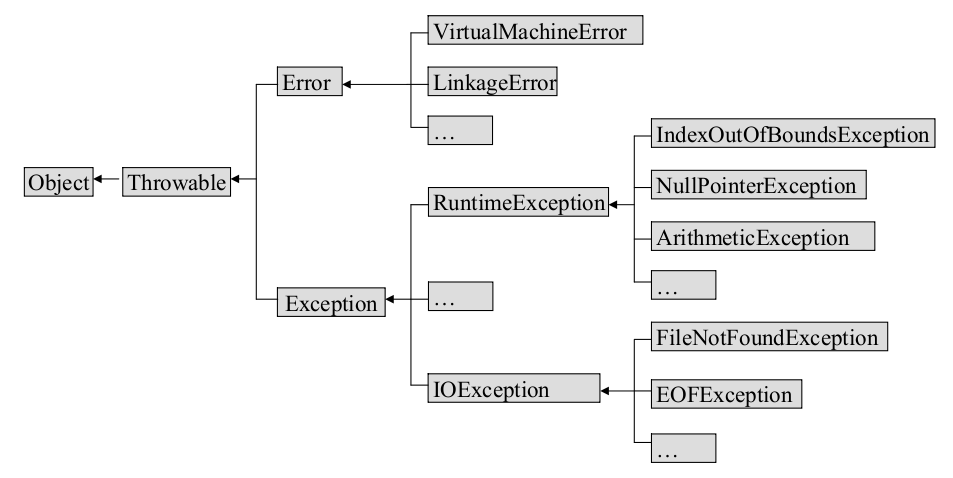
\includegraphics[width=0.95\textwidth]{images/Java-exception-handling/fig-exception-class.png}
\caption{Java异常分类}
\label{fig:exception-class}
\end{figure}

\subsection{常见错误}

\subsubsection{链接错误(LinkageError)}

LinkageError是指程序链接错误。例如,一个类中用到另外一个类,在编译前一
个类之后,后一个类发生了不相容的改变时,再使用前一个类则会出现链接错误。
最常见的就是后一个类的.class文件被误删除。

\subsubsection{虚拟机错误(VirtualMachineError)}
 
当Java虚拟机崩溃或用尽了它继续操作所需的资源时,会抛出该错误。其中比较
有代表性的是StackOverflowError,当应用程序递归太深而导致栈内存溢出时会
出现该异常。

\samplecode{TestVMerror.java}

\begin{javaCode}
  public class TestVMError {
    public static void main(String[] args) {
      TestVMError t = new TestVMError();
      t.f(100000);
    }
    public int f(int n) {
      if (n <= 0) {
        return 0;
      }
      int k = n * this.f(n-1);
      return k;
    }
  }
\end{javaCode}

标准输出如下:

\begin{stdoutCode}
  Exception in thread "main" java.lang.StackOverflowError
  at TestException.f(TestException.java:7)
  at TestException.f(TestException.java:10)  
\end{stdoutCode}

\subsection{常见异常}

\subsubsection{运行时异常(RuntimeException)}

运行时异常主要包括:

\begin{itemize}
\item 错误的类型转换;
\item 数组下标越;
\item 空指针访问。
\end{itemize}

其中,空指针异常(NullPointerException)是如果试图访问不指向任何对象的
引用变量的成员,将会产生空指针异常。例如:

\begin{javaCode}
Person p = null;
System.out.println(p.age);  
\end{javaCode}

\subsubsection{IO异常(IOException)}

\begin{itemize}
\item 从一个不存在的文件中读取数据;
\item 越过文件结尾继续读取;
\item 连接一个不存在的URL。
\end{itemize}

以下给出IOException的一个示例,注意下述代码无法通过编译!

\samplecode{TestIOException.java}

\begin{javaCode}
import java.io.*;
public class TestIOException {
  public static void main(String[] args) {
    FileInputStream in = new FileInputStream("myfile.txt");
    int b;
    b = in.read();
    while (b != -1) {
      System.out.print((char) b);
      b = in.read();
    }
    in.close();
  }
}  
\end{javaCode}

\notice{对上述代码无法编译的解释}

只要是有可能出现IOException的Java代码,在编译时就会出错,而不会等到运行
时才发生。编译出错信息大致如下:

\begin{stdoutCode}
TestIOException.java:4: 未报告的异常 java.io.FileNotFoundException; 
必须对其进行捕捉或声明以便抛出
    FileInputStream in = new FileInputStream("myfile.txt");
... ...
\end{stdoutCode}

\section{Java异常处理机制}

Java异常处理的宗旨包括:

\begin{itemize}
\item 返回到一个安全和已知的状态;
\item 能够使用户执行其他的命令;
\item 如果可能,则保存所有的工作;
\item 如果有必要,可以退出以避免造成进一步的危害。
\end{itemize}

Java异常处理的基本机制是:

\begin{itemize}
\item Java程序执行过程中如出现异常,系统会监测到并自动生成一个相应的异常类对象,然后再将它
  交给运行时系统;
\item 运行时系统再寻找相应的代码来处理这一异常。如果Java运行时系统找不到可以处理异常的代
  码,则运行时系统将终止,相应的Java程序也将退出。
\item 程序本身通常对错误(Error)无能为力,因而一般只处理违例(Exception)。
\end{itemize}

\subsection{捕获异常}

Java语言捕获异常的基本程序逻辑结构如下:

\begin{javaCode}
try {
  ... //可能产生异常的代码
} catch (ExceptionName1 e) {
  ... //当产生 ExceptionName1 型异常时的处置措施
} catch (ExceptionName2 e) {
  ... //当产生 ExceptionName2 型异常时的处置措施
} finally {
  ... //无条件执行的语句
}
\end{javaCode}

以下给出一段捕获处理数组访问越界异常的示例:

\samplecode{ArrayIndexOutOfBoundsExceptionSample.java}

\begin{javaCode}
public class ArrayIndexOutOfBoundsExceptionSample {
  public static void main(String[] args) {
    String friends[]={"Lisa","Billy","Kessy"};
    try {
      for(int i = 0; i < 5; i++) {
        System.out.println(friends[i]);
      }
    } catch(ArrayIndexOutOfBoundsException e) {
      System.out.println("index err");
    }
    System.out.println("\nthis is the end");
  }
}
\end{javaCode}

\subsection{使用finally语句}

Java异常处理中,finally语句是可选的,其作用是为异常处理提供一个统一的出口,使得在控制流转到程序的其他部分以前,能够对程序的状态作统一的管理。

\samplecode{FinallySample.java}

\begin{javaCode}
public class FinallySample {
  public static void main(String[] args) {
    String friends[]={"Lisa","Billy","Kessy"};
    try {
      for (int i = 0; i < 5; i++) {
        System.out.println(friends[i]);
      }
    } catch(ArrayIndexOutOfBoundsException e) {
      System.out.println("index err");
      return;
    } finally {
      System.out.println("in finally block!");
    }
    System.out.println("this is the end");
  }
}
  
\end{javaCode}

注意,不论try代码块中是否发生了异常事件,finally块中的语句都会被执行。当catch语句块中出现return
语句时,finally语句块同样会执行。上述代码的输出:

\begin{stdoutCode}
Lisa
Billy
Kessy
index err
in finally block!  
\end{stdoutCode}

\subsection{操纵异常对象}

发生异常时,系统将自动创建异常类对象,并将作为实参传递给匹配的catch语句块的形参,这样我们
就可以在语句块中操纵该异常对象了。主要使用异常类的父类Throwable中定义的两个成员方法:

\begin{itemize}
\item public String getMessage() 返回描述当前异常的详细消息字符串;
\item public void printStackTrace() 用来跟踪异常事件发生时运行栈的内容,并将相关信息输出
  到标准错误输出设备。本方法比较常用,在没有找到适合的异常处理代码时,系统也会自动调用该
  方法输出错误信息。
\end{itemize}

可以参考以下代码追踪运行栈信息:

\samplecode{A.java}

\begin{javaCode}
public class A {
  public void work(int[] a) {
    String s = this.contain(a, 3);
    System.out.println("Result: " + s);
  }

  public String contain(int[] source, int dest) {
    String result = "no!";
    try {
      for (int i = 0; i < source.length; i++) {
        if (source[i] == dest)
        result = "yes!";
      }
    } catch(Exception e) {
      System.out.println("异常信息:" + e.getMessage());
      System.out.println("运行栈信息:");
      e.printStackTrace();
      result = "error!";
    }
    return result;
  }
}
\end{javaCode}

\samplecode{MyTest.java}

\begin{javaCode}
public class MyTest {
  public static void main(String[] args) {
    A tst = new A();
    tst.work(null);
  }
}
\end{javaCode}

程序输出结果如下:

\begin{stdoutCode}
Exception Message: null
Stack Trace:
java.lang.NullPointerException
    at A.contain(A.java:9)
    at A.work(A.java:3)
    at MyTest.main(MyTest.java:4)
Result: error!
\end{stdoutCode}

\subsection{捕获和处理IOException}

以下给出捕获和处理IOException的示例:

\samplecode{TestIOException.java}

\begin{javaCode}
import java.io.*;
public class TestIOException {
  public static void main(String[] args) {
    try {
      FileInputStream in = new FileInputStream("myfile.txt");
      int b;
      b = in.read();
      while(b != -1) {
        System.out.print((char) b);
        b = in.read();
      }
      in.close();
    } catch (FileNotFoundException e) {
      System.out.println("File is missing!");
    } catch (IOException e) {
      e.printStackTrace();
    }
    System.out.println("It's ok!");
  }
}
\end{javaCode}

FileNotFoundException是IOException的子类,基于多态性机制,后一个catch语
句也可以处理FileNotFoundException,因此前一个catch语句块可以取消,但这
样就无法区分是“文件不存在”引发异常或其他I/O异常了。

\notice{异常处理知识点}

\begin{enumerate}
\item 对于只可能产生RuntimeException的代码可以不使用try-catch语句进行处
  理,如果对于这些相对安全的代码仍然采用了try语句块的形式,则try后可以
  省略catch语句块或finally语句块,但不能同时省略。
\item 如果试图捕获和处理代码中根本不可能出现的异常,编译器也会指出这种
  不当行为。
\end{enumerate}

\subsection{声明抛出异常}
 
声明抛弃异常是Java中处理违例的第二种方式如果。一个方法中的代码在运行时
可能生成某种异常,但在本方法中不必、或者不能确定如何处理此类异常时,则
可以声明抛弃该异常;此时方法中将不对此类异常进行处理,而是由该方法的调用
者负责处理。 语法格式如下:

\begin{javaCode}
  [< 修饰符 >] < 返回值类型 > < 方法名 > (< 参数列表 >) [throws < 异常类型 > [,< 异常类型 >]*] {
    [< Java语句 >]*
  }
\end{javaCode}

\samplecode{TestThrowsException.java}

\begin{javaCode}
import java.io.*;
public class TestThrowsException {
  public static void main(String[] args) {
    TestThrowsException t = new TestThrowsException();
    try {
      t.readFile();
    } catch (IOException e) {
      System.out.println(e);
    }
  }
  public void readFile() throws IOException {
    FileInputStream in = new FileInputStream("myfile.txt");
    int b;
    b = in.read();
    while (b != -1) {
      System.out.print((char) b);
      b = in.read();
    }
    in.close();
  }
}
\end{javaCode}
 
\notice{声明抛出异常的注意事项}

\begin{enumerate}
\item 除非事先约定,否则在开发过程中不要在自己编写的方法中采用抛出异常
  的方式。
\item 重写方法不允许抛出比被重写方法范围更大的异常类型。例
  如 IOException重写后抛出FileNotFoundException和EOFException被允许,而
  抛出Exception则不被允许。
\end{enumerate}
 
\subsection{人工抛出异常}

Java异常类对象除了在程序运行出错时由系统自动生成并抛出之外,也可根据需
要人工创建并抛出:

\begin{javaCode}
IOException e = new IOException(); // 创建异常类对象
throw e; // 抛出操作,即将该异常对象提交给Java运行环境
\end{javaCode}

被抛出的必须是Throwable或其子类类型的对象。例如,下述语句因为人工抛出的
并非Throwable或其子类的对象,在编译时会产生语法错误:

\begin{javaCode}
throw new String("want to throw");  
\end{javaCode}

以下给出一个人工抛出异常的示例:

\samplecode{TextThrowException.java}

\begin{javaCode}
import java.util.Scanner;

public class TestThrowException {
  public static void main(String[] args) {
    TestThrowException t = new TestThrowException();
    System.out.print("Please input your age: ");
    System.out.print("Your age: " + t.inputAge());
  }
  public int inputAge() {
    int result = -1;
    Scanner scan = new Scanner(System.in);
    while (true) {
      try {
        result = scan.nextInt();
        if (result < 0 || result > 130) {
          Exception me = new Exception("You come from Mars? ");
          throw me;
        }
        break;
      } catch (Exception e1) {
        System.out.println(e1.getMessage() + "Please input your age again: ");
        continue;
      }
    }
    return result;
  }
}
\end{javaCode}

上述代码所述的情况利用异常处理机制实现数据取值范围的检查并不太合适。应
用异常处理机制的原则如下:

\begin{itemize}
\item 当明确知道可能出错的地方或能够通过简单的检查而有效防止错误发生,
  就应该使用if-else语句来预防错误发生;
\item 只有当我们无法明确知道错误发生之处或无法完全避免异常,才不得不通
  过异常处理的方式来捕获和处理异常。
\end{itemize}


\section{用户自定义异常}

Java语言及许多类库针对常见异常状况已事先定义了相应的异常类型,并在程序
运行出错时由系统自动创建相应异常对象并进行抛出、捕获和处理,因此一般不
需要用户人工抛出异常对象或定义新的异常类型,但针对特殊的需要也可以这样
做。

我们一般通过继承Exception类来实现异常类型自定义,由于用户自定义的异常不
会由系统自动检测并抛出,所以只能靠人工触发并抛出。

以下给出用户自定义异常的示例:

\samplecode{CustomizingException.java}

\begin{javaCode}
public class CustomizingException extends Exception {
  private int idnumber;

  public MyException(String message, int id) {
    super(message);
    this.idnumber = id;
  }

  public int getId() {
    return idnumber;
  }
}
\end{javaCode} 

上述自定义异常类代码的构造方法中使用super调用其父类Exception的有参构造
方法,以便在创建异常对象时将用户的定制的报错信息传递给父类中定义
的private属性Message(该属性由Throwable类定义),将来在捕获和处理异常时
就可以通过调用该对象的getMessage()方法访问到该信息。

\samplecode{TestCustomizingException.java}

\begin{javaCode}
public class TestCustomizingException {
  public void regist(int num) throws MyException {
    if (num < 0) {
      throw new MyException("人数为负值,不合理", 3);
    }
    System.out.println("登记人数:" + num);
  }

  public void manager() {
    try {
      regist(-100);
    } catch (MyException e) {
      System.out.println("登记失败,出错种类" + e.getId());
      e.printStackTrace();
    }
    System.out.print("本次登记操作结束");
  }

  public static void main(String args[]) {
    new TestCustomizingException().manager();
  }
}
\end{javaCode}

上述测试程序输出结果如下:

\begin{stdoutCode}
登记失败,出错种类3
MyException: 人数为负值,不合理 ...
\end{stdoutCode}

\section{断言}

\subsection{什么是断言}

从JDK1.4版本开始,Java语言中引入了断言(Assert)机制,允许Java开发者在
代码中加入一些检查语句,主要目的是用于程序调试。

\begin{itemize}
\item 当我们需要在约定的条件不成立时中断当前程序执行操作的话可以使用断言;
\item 使用断言是为了在测试阶段确定程序内部出错位置和出错信息,而不是控制程序流程;
\item 断言机制在用户定义的boolean表达式(判定条件)结果为false时抛出一
  个Error对象,其类型为AssertionError;
\item 作为Error的一种,断言失败也不需捕获处理或者声明抛出,一旦出现了则
  终止程序、不必进行补救和恢复。

\end{itemize}

\subsection{启用和禁用断言}

\subsubsection{命令行开启断言功能}

Java运行时环境默认设置为关闭断言功能,因此在使用断言以前,需要在运
行Java程序时先开启断言功能。方法如下:

\begin{shCode}
>java -ea MyAppClass
\end{shCode}

或者:

\begin{shCode}
>java -enableassertions MyAppClass  
\end{shCode}

\subsubsection{命令行关闭断言功能}

\begin{shCode}
>java -da MyAppClass  
\end{shCode}

或者:

\begin{shCode}
java -disableassertions MyAppClass  
\end{shCode}

\subsubsection{Eclipse IDE开启断言}

在项目上点击右键 \ding{224} Run As \ding{224} Run Configurations \ding{224} Arguments,
在VM arguments中,加入-enableassertions或-ea即可。

\subsection{使用断言}

第一种断言的语法格式如下:

\begin{javaCode}
assert <boolean 表达式>;  
\end{javaCode}

以下给出使用第一种断言语法的示例代码:

\samplecode{TestAssertion.java}

\begin{javaCode}
public class TestAssertion {
  public static void main(String[] args) {
    new TestAssertion().process(-12);
  }
  public void process(int age) {
    assert age >= 0;
    System.out.println("您的年龄:" + age);
    // ---
  }
}
\end{javaCode}

以上程序执行的输出如下:

\begin{stdoutCode}
Exception in thread "main" java.lang.AssertionError
	at TestAssertion.process(TestAssertion.java:8)
	at TestAssertion.main(TestAssertion.java:4)  
\end{stdoutCode}

第二种断言的语法格式如下:

\begin{javaCode}
assert < boolean 表达式 >:< 表达式 2 >;  
\end{javaCode}

以下给出第二种断言格式的示例代码:

\samplecode{TestAssertion2.java}

\begin{javaCode}
public class TestAssertion2 {
  public static void main(String[] args) {
    new TestAssertion2().process(-12);
  }
  public void process(int age) {
    assert age >= 0: "年龄值不合理";
    System.out.println("您的年龄:" + age);
    //---
  }
}
\end{javaCode}

输出结果如下:

\begin{stdoutCode}
Exception in thread "main" java.lang.AssertionError: 年龄值不合理
	at TestAssertion.process(TestAssertion.java:8)
	at TestAssertion.main(TestAssertion.java:4)  
\end{stdoutCode}

\descript{说明}

断言失败时,系统会自动将表达式2的值传递给新创建的AssertionError对象,进
而将其转换为一个消息字符串保存起来,这样就可以在获得更多/更有针对性的检
查失败细节信息。因此,其中的表达式2可以是任何基本数据类型或引用数据类型,
但必须提供一个值,即不能为空值。

\section{课后习题}

\begin{enumerate}
\item 总结Java的异常处理机制。
\item 什么是运行时异常?
\item 若try语句结构中有多个catch()子句,这些子句的排列顺序与程序执行效果是否有关?
\item 总结Java异常处理机制随Java版本的更新不断加入的新特性,并附参考文献或网站链接。(选做)
\end{enumerate}
% \chapter*{线程编程}
\label{chp:Java-thread-programming}

\section*{本章要点}

\sline
\begin{enumerate}
\item 线程的基础概念;
\item 线程的控制;
\item 线程的同步。
\end{enumerate}  
\sline

\section{线程基础}

\subsection{进程}

进程是一个具有一定独立功能的程序在一个数据集上的一次动态执行的过程,是
操作系统进行资源分配和调度的一个独立单位,是应用程序运行的载体。进程是
一种抽象的概念,从来没有统一的标准定义。进程一般由程序、数据集合和进程
控制块三部分组成。程序用于描述进程要完成的功能,是控制进程执行的指令集;
数据集合是程序在执行时所需要的数据和工作区;进程控制块(Program Control
Block,简称PCB),包含进程的描述信息和控制信息,是进程存在的唯一标志。

进程具有的特征:

\begin{description}
\item[动态性] 进程是程序的一次执行过程,是临时的,有生命期的,是动态产
  生,动态消亡的;
\item[并发性] 任何进程都可以同其他进程一起并发执行;
\item[独立性] 进程是系统进行资源分配和调度的一个独立单位;
\item[结构性] 进程由程序、数据和进程控制块三部分组成。
\end{description}

\subsection{什么是线程}

根据多任务原理,在一个程序内部也可以实现多个任务(顺序控制流)的并发执
行,其中每个任务被称为线程(Thread)。更专业的表述为:{\hei 线程是程序
  内部的顺序控制流。}

\sline

在早期的操作系统中并没有线程的概念,进程是能拥有资源和独立运行的最小单
位,也是程序执行的最小单位。任务调度采用的是时间片轮转的抢占式调度方式,
而进程是任务调度的最小单位,每个进程有各自独立的一块内存,使得各个进程
之间内存地址相互隔离。

后来,随着计算机的发展,对CPU的要求越来越高,进程之间的切换开销较大,已
经无法满足越来越复杂的程序的要求,于是就发明了线程。线程是程序执行中一
个单一的顺序控制流程,是程序执行流的最小单元,是处理器调度和分派的基本
单位。一个进程可以有一个或多个线程,各个线程之间共享程序的内存空间(也
就是所在进程的内存空间)。一个标准的线程由线程ID、当前指令指针(PC)、
寄存器和堆栈组成。而进程由内存空间(代码、数据、进程空间、打开的文件)
和一个或多个线程组成。

线程是进程的一个实体,是CPU调度和分派的基本单位,它是比进程更小的能独立
运行的基本单位。线程自己只拥有一点在运行中必不可少的资源(如程序计数器,
一组寄存器和栈),但是它可与同属一个进程的其他的线程共享进程所拥有的全
部资源。

\sline

\subsection{线程和进程的区别}

进程和线程都是由操作系统所体现的程序运行的基本单元,系统利用该基本单元
实现系统对应用的并发性。从逻辑角度来看,多线程的意义在于一个应用程序中,
有多个执行部分可以同时执行。但操作系统并没有将多个线程看做多个独立的应
用,来实现进程的调度和管理以及资源分配。进程和线程的区别有:

\begin{enumerate}
\item 每个进程都有独立的代码和数据空间(进程上下文),进程切换的开销
  大。
\item 线程作为轻量的“进程”,同一类线程共享代码和数据空间,每个线程有独立
  的运行栈和程序计数器(PC),线程切换的开销小。
\item 多进程——在操作系统中能同时运行多个任务(程序)。
\item 多线程——在同一应用程序中有多个顺序流同时执行。
\end{enumerate}

\subsection{线程的概念模型}

在Java语言中,多线程机制通过虚拟CPU来实现。

\begin{enumerate}
\item 虚拟的CPU,由java.lang.Thread类封装和虚拟;
\item 虚拟CPU所执行的代码,传递给Thread类对象;
\item 虚拟CPU所处理的数据,传递给Thread类代码对象。
\end{enumerate}

\subsection{创建线程}

Java的线程是通过java.lang.Thread类来实现的。每个线程都是通过某个特
定Thread对象所对应的方法run()来完成其操作的,方法run()称为线程体。

以下给出一个创建线程的示例:

\samplecode{TestThread1.java}

\begin{javaCode}
public class TestThread1 {
  public static void main(String args[]) {
    Runner1 r = new Runner1();
    Thread t = new Thread(r);
    t.start();
  }
}

class Runner1 implements Runnable {
  public void run() {
    for(int i=0; i<30; i++) {
      System.out.println("No. " + i);
    }
  }
}
\end{javaCode}

参考以上代码,给出创建和启动线程的一般步骤:

\begin{enumerate}
\item 定义一个类实现Runable接口,重写其中的run()方法,加入所需的处理逻辑;
\item 创建Runable接口实现类的对象;
\item 创建Thread类的对象(封装Runable接口实现类型对象);
\item 调用Thread对象的start()方法,启动线程。
\end{enumerate}

\subsection{多线程的目标}

Java中引入线程机制的目的在于实现{\hei 多线程(Multi-Thread)}并发的任务
执行。以下代码基于同一个线程体创建并运行两个线程,基于线程体共享和主线
程初始对象共享,多线程之间可以共享代码和数据。

\begin{table}[!htbp]
\centering
%\caption{}
%\label{tab:}
\begin{tabular}{|c|c|c|c|}
  \hline
  {\bf 线程} & {\bf 虚拟CPU} & {\bf 代码} & {\bf 数据} \\
  \hline
  t1 & Thread类对象 & Runner2类中的run()方法 & Runnable类型对象r \\
  \hline
  t2 & Thread类对象 & Runner2类中的run()方法 & Runnable类型对象r \\
  \hline
\end{tabular}
\end{table}

\samplecode{TestThread2.java}

\begin{javaCode}
public class TestThread2 {
  public static void main(String args[]) {
    Runner2 r = new Runner2();
    Thread t1 = new Thread(r);
    Thread t2 = new Thread(r);
    t1.start();
    t2.start();
  }
}

class Runner2 implements Runnable {
  public void run() {
    for(int i=0; i<20; i++) {
      String s = Thread.currentThread().getName(); //获取当前运行中的线程对象
      System.out.println(s + ": " + i);
    }
  }
}
\end{javaCode}

\subsection{创建线程的第二种方式}

可以直接继承Thread类创建线程。

\begin{enumerate}
\item 定义一个类继承Thread类,重写其中的run()方法,加入所需的处理逻辑;
\item 创建该Thread类的对象;
\item 调用该对象的start()方法。
\end{enumerate}

以下给出示例代码:

\samplecode{TestThread3.java}

\begin{javaCode}
public class TestThread3 {
  public static void main(String args[]) {
    Thread t = new Runner3();
    t.start();
  }
}

class Runner3 extends Thread {
  public void run() {
    for(int i=0; i<30; i++) {
      System.out.println("No. " + i);
    }
  }
}
\end{javaCode}


\subsection{两种创建线程的方式比较}

\subsubsection{使用Runnable接口创建线程}

\begin{itemize}
\item 可以将虚拟CPU、代码和数据分开,形成清晰的模型;
\item 线程体run()方法所在的类还可以从其他类继承一些有用的属性或方法;
\item 有利于保持程序风格的一致性。
\end{itemize}

\subsubsection{直接继承Thread类创建线程}

\begin{itemize}
\item Thread子类无法再从其他类继承;
\item 编写简单,run()方法的当前对象就是线程对象,可直接操作。
\end{itemize}

\subsection{后台线程}

\subsubsection{相关概念}
\begin{description}
\item[后台处理] 也称为后台运行,是指在分时处理或多任务系统中,当实时、会话式、高优先级或需
迅速相应的计算机程序不再使用系统资源时,计算机去执行较低优先级程序的过程。批量处理、文件
打印通常采取后台处理的形式。
\item[后台线程] 是指那些在后台运行的,为其他线程提供服务的功能,如JVM的垃圾回收线程等,后
台线程也称为守护线程(Daemon Thread)。
\item[用户线程] 和后台线程相对应,其他完成用户任务的线程可称为“用户线程”。
\end{description}

Thread类提供的与后台线程相关的方法包括:

\begin{enumerate}
\item 测试当前线程是否为守护线程,如果是则返回true,否则返回false。
\begin{javaCode}
public final boolean isDaemon();
\end{javaCode}
\item 将当前线程标记为守护线程或用户线程,本方法必须在启动线程前调用。
\begin{javaCode}
public final void setDaemon(Boolean on);
\end{javaCode}
\end{enumerate}

以下给出使用后台线程的示例:

\samplecode{TestDaemonThread.java}

\begin{javaCode}
public class TestDaemonThread {
  public static void main(String[] args) {
    Thread t1 = new MyRunner(10);
    t1.setName("用户线程t1");
    t1.start();
    Thread t2 = new MyRunner(10000);
    t2.setDaemon(true);
    t2.setName("后台线程t2");
    t2.start();
    for(int i = 0; i < 10; i++) {
      System.out.println(Thread.currentThread().getName() + ": " + i);
    }
    System.out.println("主线程结束");
  }
}

class MyRunner extends Thread {
  private int n;
  public MyRunner(int n) {
    this.n = n;
  }
  public void run() {
    for(int i = 0; i < n; i++) {
      System.out.println(this.getName() + ": " + i);
    }
    System.out.println(this.getName() + "结束");
  }
}  
\end{javaCode}

\descript{对上述代码的说明}

后台线程线程t2并没有如预期的输出数字$0$-$9999$,而是提前终止。这是因为,
待用户线程(这里包括主线程和线程t1)全部运行结束后,JVM检测到只剩下后台
线程在运行的时候,就退出了当前应用程序的运行。

请将上述代码中的“t2.setDaemon(true);”注释后,编译运行程序进行比较运行结果。


\subsection{GUI线程}

GUI程序运行过程中,系统会自动创建若干个GUI线程以提供所需的功能,主要包
括{\Blue\hei 窗体显示和重绘、GUI事件处理、关闭抽象窗口工具集等}。

\begin{description}
\item[AWT-Windows线程] 负责从操作系统获取底层事件通知,并将之发送到系统
  事件队列(EventQueue)等待处理。在其他平台上运行时,此线程的名字也会
  作相应变化,例如在Unix系统则为“AWT-Unix”。
\item[AWT-EventQueue-n线程] 也称事件分派线程,该线程负责从事件队列中获
  取事件,将之分派到相应的GUI组件(事件源)上,进而触发各种GUI事件处理
  对象,并将之传递给相应的事件监听器进行处理。
\item[AWT-Shutdown线程] 负责关闭已启用的抽象窗口工具,释放其所占用的资
  源,该线程将等到其他GUI线程均退出后才开始其清理工作。
\item[DestroyJavaVM线程] 在所有其他用户线程退出后,负责释放任意线程所占
  用系统资源并卸载Java虚拟机。该线程在主线程运行结束时由系统自动启动,
  但要等到所有其他用户线程均退出后才开始其卸载工作。
\end{description}

以下给出测试GUI线程的示例:

\samplecode{TestGUIThread.java}

\begin{javaCode}
import java.awt.*;
import java.awt.event.*;

public class TestGUIThread {
  public static void main(String[] args) throws Exception {
    Frame f = new Frame();
    Button b = new Button("Press Me");
    MyMonitor mm = new MyMonitor();
    b.addActionListener(mm);
    f.addWindowListener(mm);
    f.add(b, "Center");
    f.setSize(100, 60);
    f.setVisible(true);
    MyThreadViewer.view();
  }
}

class MyMonitor extends WindowAdapter implements ActionListener {
  public void actionPerformed(ActionEvent e) {
    MyThreadViewer.view();
  }
}

class MyThreadViewer {
  public static void view() {
    Thread current = Thread.currentThread();
    System.out.println("当前线程名称:" + current.getName());
    int total = Thread.activeCount();
    System.out.println("活动线程总数:" + total + "个");
    Thread[] threads = new Thread[total];
    current.enumerate(threads);
    for(Thread t: threads) {
      String role = t.isDaemon() ? "后台线程" : "用户线程";
      System.out.println("   -" + role + t.getName());
    }
    System.out.println("-------------------");
  }
}
\end{javaCode}


%% [API] Thread.enumerate
%% 
%% Copies into the specified array every active thread in the current thread's thread group
%% and its subgroups. This method simply calls the enumerate method of the current thread's
%% thread group with the array argument.
%% 
%% First, if there is a security manager, that enumerate method calls the security
%% manager's checkAccess method with the thread group as its argument. This may result in
%% throwing a SecurityException.
%% 
%% Parameters: 
%% \begin{itemize}
%% \item tarray an array of Thread objects to copy to
%% \end{itemize}
%% Returns: 
%% \begin{itemize}
%% \item the number of threads put into the array
%% \end{itemize}
%% Throws:
%% \begin{itemize}
%% \item SecurityException - if a security manager exists and its checkAccess method
%%   doesn't allow the operation.
%% \end{itemize}

\section{线程控制}

\subsection{线程的生命周期}

线程的生命周期包含以下5个状态(状态间关系如图\ref{fig:thread-lifecycle}所示):

\begin{description}
\item[新建状态] 调用Thread构造方法,未显式调用start()方法前;
\item[就绪状态] 调用start()方法后,线程在就绪队列里等候;
\item[运行状态] 开始执行线程体代码;
\item[阻塞状态] 因某事件发生,例如线程进行I/O操作,等待用户输入数据;
\item[终止状态] 线程run()方法执行完毕。
\end{description}

\begin{figure}[h]
\centering
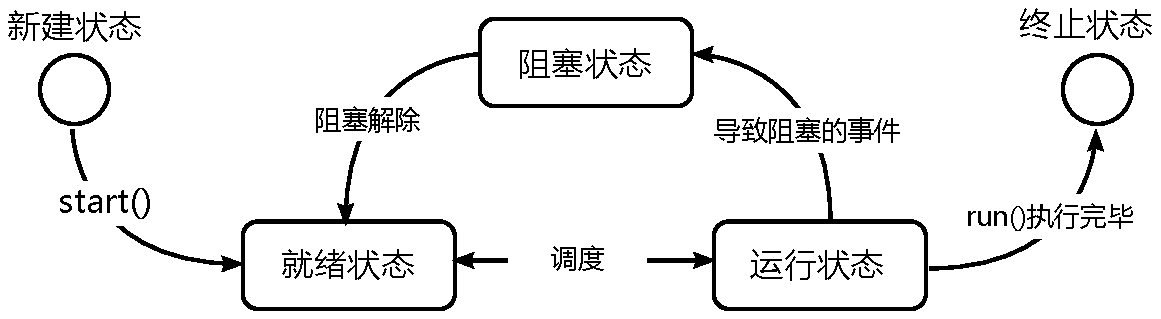
\includegraphics[width=0.95\textwidth]{images/fig-thread-lifecycle.pdf}
\caption{Java线程生命周期状态}
\label{fig:thread-lifecycle}
\end{figure}

\subsection{线程优先级}

线程的优先级用数字来表示,范围从1到10。主线程的缺省优先级是5,子线程的
优先级默认与其父线程相同。可以使用Thread类的下述方法获得和设置线程的优
先级。

\begin{itemize}
\item 获取当前线程优先级
  \begin{javaCode}
    public final int getPriority();
  \end{javaCode}
\item 设定当前线程优先级
  \begin{javaCode}
    public final void setPriority(int newPriority);
  \end{javaCode}
\end{itemize}

相关静态整型常量如下:

\begin{javaCode}
Thread.MIN_PRIORITY = 1
Thread.MAX_PRIORITY = 10
Thread.NORM_PRIORITY = 5
\end{javaCode}

\subsection{线程串行化}

在多线程程序中,如果在一个线程运行的过程中要用到另一个线程的运行结果,
则可进行线程的串型化处理。

Thread类提供的线程串行化相关方法包括:

\begin{javaCode}
public final void join();
public final void join(long millis);
public final void join(long millis, int nanos);
\end{javaCode}

以下给出实现线程串行化的代码示例:

\samplecode{TestJoin.java}

\begin{javaCode}
public class TestJoin {
  public static void main(String[] args) {
    MyRunner r = new MyRunner();
    Thread t = new Thread(r);
    t.start();
    try {
      t.join();
    } catch(InterruptedException e) {
      e.printStackTrace();
    }
    for(int i = 0; i < 50; i++) {
      System.out.println("主线程:" + i);
    }
  }
}

class MyRunner implements Runable {
  public void run() {
    for(int i = 0; i < 50; i++) {
      System.out.println("子线程:" + i);
  }
}
\end{javaCode}

\descript{说明}

上述程序中,主线程在执行过程中调用了线程t的join()方法,该方法导致当前线程(主线程)阻塞,直
到线程t运行终止后,主线程才会获得继续执行的机会。这相当于将线程t串行加入到主线程中。

\subsection{线程休眠}

线程休眠,即暂停执行当前运行中的线程,使之进入阻塞状态,待经过指定
的“延迟时间”后再醒来并转入到就绪状态。

Thread类提供的线程休眠相关方法包括:

\begin{javaCode}
public static void sleep(long millis);
public static void sleep(long millis, int nanos);
\end{javaCode}

以下给出使用线程休眠实现的数字计数器示例:

\samplecode{Digitaltimer.java}

\begin{javaCode}
import java.util.Calendar;
import java.util.GregorianCalendar;
import javax.swing.*;

public class DigitalClock {
  public static void main(String[] args) {
    JFrame jf = new JFrame("Clock");
    JLabel clock = new JLabel("clock");
    clock.setHorizontalAlignment(JLabel.CENTER);
    jf.add(clock, "Center");
    jf.setSize(140, 80);
    jf.setLocation(500, 300);
    jf.setDefaultCloseOperation(JFrame.EXIT_ON_CLOSE);
    jf.setVisible(true);
    Thread t = new MyThread(clock);
    t.start();
  }
}

class MyThread extends Thread {
  private JLabel clock;
  private int i;
  public MyThread(JLabel clock) {
    this.clock = clock;
    this.i = 1;
  }
  public void run() {
    while(true) {
      clock.setText(String.valueOf(i++));
      try {
        Thread.sleep(1000);
      } catch(InterruptedException e) {
        e.printStackTrace();
      }
    }
  }
}  
\end{javaCode}

\subsection{线程让步}

线程让步,让运行中的线程主动放弃当前获得的CPU处理机会,但不是使该线程阻
塞,而是使之转入就绪状态。Thread类提供的线程让步相关方法:

\begin{javaCode}
public static void yield();
\end{javaCode}

以下给出一个线程让步的示例:

\samplecode{TestYield.java}

\begin{javaCode}
import java.util.Date;

public class TestYield {
  public static void main(String[] args) {
    Thread t1 = new MyThread(false);
    Thread t2 = new MyThread(true);
    Thread t3 = new MyThread(false);
    t1.start();
    t2.start();
    t3.start();
  }
}

class MyThread extends Thread {
  private boolean flag;
  public MyThread(boolean flag) {
    this.flag = flag;
  }
  public void setFlag(boolean flag) {
    this.flag = flag;
  }
  public void run() {
    long start = new Date().getTime();
    for(int i = 0; i < 200; i++) {
      if(flag) {
        Thread.yield();
      }
      System.out.println(this.getName() + ": " + i + "\t");
    }
    long end = new Date().getTime();
    System.out.println("\n" + this.getName() + "执行时间:" + (end - start) + "ms");
  }
}
\end{javaCode}

从执行结果来看,由于设置了线程让步,第二个线程明显执行时间长。调
用yield()方法只是令当前线程主动在时间片到期前使其他线程获得运行机会。

\subsection{线程挂起与恢复}

\begin{description}
\item[线程挂起] 暂时停止当前运行中的线程,使之转入阻塞状态,并且不会自动恢复运行。
\item[线程恢复] 使得一个已挂起的线程恢复运行。
\end{description}

Thread类提供的线程挂起与恢复的相关方法:

\begin{javaCode}
public final void suspend();
public final void resume();
\end{javaCode}

suspend()和resume()方法已经不提倡使用,原因是suspend()方法挂起线程时并不释放其锁定的资
源,这可能会影响到其他线程的执行,且容易导致线程死锁。

\subsection{线程等待与通知}

将运行中的线程转为阻塞状态的另外一种途径是:调用该线程中被锁定资源
(Java对象)的wait()方法,该方法在Object类中定义,其功能是让当前线程等
待,直到有其他线程调用了同一个对象的notify()或notifyAll()方法通知其结束
等待,或是经历了约定的等待时间后,等待线程才会醒来,重新进入可执行状
态。
 
线程等待与线程挂起比较:

\begin{itemize}
\item 线程挂起时不会释放所占用的资源;
\item 线程等待时则会释放资源,以使其他线程获得运行机会。
\end{itemize}

\section{线程的同步}

\subsection{临界资源问题}

两个线程A和B在同时操纵Stack类的同一个实例(栈),A向栈里push一个数据,B要从堆栈中pop一个数据。

\samplecode{Stack.java}

\begin{javaCode}
public class Stack {
  int idx = 0;
  char[] data = new char[6];
  
  public void push(char c) {
    data[idx] = c;
    idx++;
  }
  public char pop() {
    idx--;
    return data[idx];
  }
}
\end{javaCode}

\descript{上述问题分析}

\begin{enumerate}
\item 操作之前,假设data = |a|b| | | | |,idx = 2;
\item 线程A执行push中的第一个语句,将c推入堆栈; data = |a|b|c| | | |,idx = 2;
\item 线程A还未执行idx++语句,A的执行被线程B中断,B执行pop方法,data = |a|b|c| | | | idx = 1;
\item 线程A继续执行push的第二个语句: data = |a|b|c| | | |, idx = 2;
\item 最后的结果相当于c没有入栈,产生这种问题的原因在于对共享数据访问的操作的不完整性。
\end{enumerate}

\subsection{Java synchronized}
  
synchronized是Java中的关键字,当某个对象用synchronized修饰时,表明该对
象在任一时刻只能由一个线程访问。synchronized是一种同步锁,其修饰的对象
有以下几种:

\begin{enumerate}
\item 修饰一个代码块,被修饰的代码块称为同步语句块,其作用的范围是大括
  号{}括起来的代码,作用的对象是调用这个代码块的对象;
\item 修饰一个方法,被修饰的方法称为同步方法,其作用的范围是整个方法,
  作用的对象是调用这个方法的对象;
\item 修改一个静态的方法,其作用的范围是整个静态方法,作用的对象是这个
  类的所有对象;
\item 修改一个类,其作用的范围是synchronized后面括号括起来的部分,作用
  主的对象是这个类的所有对象。
\end{enumerate}

\subsection{synchronized的用法}

synchronized用于方法声明中,标明整个方法为同步方法。

\begin{javaCode}
public synchronized void push(char c) {
  data[idx] = c;
  idx++;
}
\end{javaCode}

synchronized用于修饰语句快,标明整个语句块为同步块。

\begin{javaCode}
public char pop() {
  synchronized(this) {
    idx--;
    return data[idx];
  }
}
\end{javaCode}

\notice{线程死锁}

并发运行的多个线程间彼此等待、都无法运行的状态称为线程死锁。为避免死锁,
在线程进入阻塞状态时应尽量释放其锁定的资源,以为其他的线程提供运行的机
会。

\begin{itemize}
\item public final void wait()
\item public final void notify()
\item public final void notifyAll()
\end{itemize}

\subsection{生产者—消费者问题}

\begin{javaCode}
public class SyncStack {
  private int index = 0;
  private char[] data = new char[6];

  public synchronized void push(char c) {
    while(index == data.length) {
      try {
        this.wait();
      } catch(InterruptedException e) {
      }
    }
    this.notify();
    data[index] = c;
    index++;
    System.out.println("生产: " + c);
  }
  
  public synchronized char pop() {
    while(index == 0) {
      try {
        this.wait();
      } catch(InterruptedException e) {
      }
    }
    this.notify();
    index--;
    System.out.println("消费: " + data[index]);
    return data[index];
  }
}
\end{javaCode}

\subsubsection{生产者}
  
\begin{javaCode}
  public class Producer implements Runnable {
    SyncStack stack;
    public Producer(SyncStack s) {
      stack = s;
    }
    public void run() {
      for(int i=0; i<20; i++) {
        char c = (char)(Math.random() * 26 + 'A');
        stack.push(c);
        try {
          Thread.sleep((int)(Math.random() * 300));
        } catch(InterruptedException e) {
          e.printStackTrace();
        }
      }
    }
  }    
\end{javaCode}

\subsubsection{消费者}
  
\begin{javaCode}
  public class Consumer implements Runnable {
    SyncStack stack;
    public Consumer(SyncStack s) {
      stack = s;
    }
    public void run() {
      for(int i=0; i<20; i++) {
        char c = stack.pop();
        try {
          Thread.sleep((int)(Math.random() * 800));
        } catch(InterruptedException e) {
          e.printStackTrace();
        }
      }
    }
  }
\end{javaCode}


%%%
% \backmatter

%%%%%%%%%%%%%%%%%%%%%%%%%%%%%%%%%%%%%%%%%%%%%%%%
\end{document}
%%%%%%%%%%%%%%%%%%%%%%%%%%%%%%%%%%%%%%%%%%%%%%%%
%%%%% Thank for Teddy %%%%%